% does truven include medicare
% patient statistic at early ages
% fig 5 and 6 do not include psychiatric phenotypes?
% add older figure without psych codes to SI
%------------------------------------------
\documentclass[onecolumn,,10pt]{IEEEtran}
\let\labelindent\relax
\usepackage{enumitem}
\usepackage{etex}
\usepackage{amssymb,amsfonts,amsmath,amsthm}
\usepackage{graphicx}
\usepackage[usenames,x11names, dvipsnames, svgnames]{xcolor}
\usepackage{amsmath,amssymb}
\usepackage{dsfont}
\usepackage{amsfonts}
\usepackage{mathrsfs}
\usepackage{texshade}
\usepackage{multirow}
\usepackage{hyperref}
\hypersetup{
  colorlinks=true,
  linkcolor=black,
  citecolor=black,
  filecolor=black,
  urlcolor=DodgerBlue4,
  breaklinks=false,
  % linkbordercolor=red,% hyperlink borders will be red
  % pdfborderstyle={/S/U/W 1}% border style will be underline of width 1pt
}
\usepackage{array}
\usepackage{xr}
\usepackage{verbatim}
% \usepackage{multirow}    
% \usepackage[T1,euler-digits]{eulervm}
% \usepackage{times}
% \usepackage{pxfonts}
\usepackage{tikz}
\usepackage{pgfplots}
\usetikzlibrary{shapes,calc,shadows,fadings,arrows,decorations.pathreplacing,automata,positioning}
\usetikzlibrary{external}
\usetikzlibrary{decorations.text}
\usepgfplotslibrary{colorbrewer} 

\tikzexternalize[prefix=./Figures/External/]% activate externalization!
\tikzexternaldisable
% \addtolength{\voffset}{.1in}  
\usepackage{geometry}
\geometry{a4paper, left=.65in,right=.65in,top=.8in,bottom=0.7in}

\addtolength{\textwidth}{-.1in}    
\addtolength{\hoffset}{.05in}    
\addtolength{\textheight}{0in}    
\addtolength{\footskip}{0in}    
\usepackage{rotating}
\definecolor{nodecol}{RGB}{240,240,220}
\definecolor{nodeedge}{RGB}{240,240,225}
\definecolor{edgecol}{RGB}{130,130,130}
\tikzset{%
  fshadow/.style={      preaction={
      fill=black,opacity=.3,
      path fading=circle with fuzzy edge 20 percent,
      transform canvas={xshift=1mm,yshift=-1mm}
    }} 
}
\usetikzlibrary{pgfplots.dateplot}
\usetikzlibrary{patterns}
\usetikzlibrary{decorations.markings}
\usepackage{fancyhdr}
\usepackage{mathtools}
\usepackage{datetime}
\usepackage{comment}
%% ## Equation Space Control---------------------------
\def\EQSP{3pt}
\newcommand{\mltlne}[2][\EQSP]{\begingroup\setlength\abovedisplayskip{#1}\setlength\belowdisplayskip{#1}\begin{equation}\begin{multlined} #2 \end{multlined}\end{equation}\endgroup\noindent}
\newcommand{\cgather}[2][\EQSP]{\begingroup\setlength\abovedisplayskip{#1}\setlength\belowdisplayskip{#1}\begin{gather} #2 \end{gather}\endgroup\noindent}
\newcommand{\cgathers}[2][\EQSP]{\begingroup\setlength\abovedisplayskip{#1}\setlength\belowdisplayskip{#1}\begin{gather*} #2 \end{gather*}\endgroup\noindent}
\newcommand{\calign}[2][\EQSP]{\begingroup\setlength\abovedisplayskip{#1}\setlength\belowdisplayskip{#1}\begin{align} #2 \end{align}\endgroup\noindent}
\newcommand{\caligns}[2][\EQSP]{\begingroup\setlength\abovedisplayskip{#1}\setlength\belowdisplayskip{#1}\begin{align*} #2 \end{align*}\endgroup\noindent}
\newcommand{\mnp}[2]{\begin{minipage}{#1}#2\end{minipage}} 
%% COLOR DEFS------------------------------------------
\newtheorem{thm}{Theorem}
\newtheorem{cor}{Corollary}
\newtheorem{lem}{Lemma}
\newtheorem{prop}{Proposition}
\newtheorem{defn}{Definition}
\newtheorem{exmpl}{Example}
\newtheorem{rem}{Remark}
\newtheorem{notn}{Notation}
%% ------------PROOF INCLUSION -----------------
\def\NOPROOF{Proof omitted.}
\newif\ifproof
\prooffalse % or \draftfalse
\newcommand{\Proof}[1]{
  \ifproof
  \begin{IEEEproof}
    #1\end{IEEEproof}
  \else
  \NOPROOF
  \fi
}
%% ------------ -----------------
\newcommand{\DETAILS}[1]{#1}
%% ------------ -----------------
% color commands------------------------
\newcommand{\etal}{\textit{et} \mspace{3mu} \textit{al.}}
% \renewcommand{\algorithmiccomment}[1]{$/** $ #1 $ **/$}
\newcommand{\vect}[1]{\textbf{\textit{#1}}}
\newcommand{\figfont}{\fontsize{8}{8}\selectfont\strut}
\newcommand{\hlt}{ \bf \sffamily \itshape\color[rgb]{.1,.2,.45}}
\newcommand{\pitilde}{\widetilde{\pi}}
\newcommand{\Pitilde}{\widetilde{\Pi}}
\newcommand{\bvec}{\vartheta}
\newcommand{\algo}{\textrm{\bf\texttt{GenESeSS}}\xspace}
\newcommand{\xalgo}{\textrm{\bf\texttt{xGenESeSS}}\xspace}
\newcommand{\FNTST}{\bf }
\newcommand{\FNTED}{\color{darkgray} \scriptsize $\phantom{.}$}
\renewcommand{\baselinestretch}{.95}
\newcommand{\sync}{\otimes}
\newcommand{\psync}{\hspace{3pt}\overrightarrow{\hspace{-3pt}\sync}}
% \newcommand{\psync}{\raisebox{-4pt}{\begin{tikzpicture}\node[anchor=south] (A) {$\sync$};
%   \draw [->,>=stealth] ([yshift=-2pt, xshift=2pt]A.north west) -- ([yshift=-2pt]A.north east); %\end{tikzpicture}}}
\newcommand{\base}[1]{\llbracket #1 \rrbracket}
\newcommand{\nst}{\textrm{\sffamily\textsc{Numstates}}}
\newcommand{\HA}{\boldsymbol{\mathds{H}}}
\newcommand{\eqp}{ \vartheta }
\newcommand{\entropy}[1]{\boldsymbol{h}\left ( #1 \right )}
\newcommand{\norm}[1]{\left\lVert #1 \right\rVert}%
\newcommand{\abs}[1]{\left\lvert #1 \right\rvert}%
\newcommand{\absB}[1]{\big\lvert #1 \big\rvert}%
% #############################################################
% #############################################################
% PREAMBLE ####################################################
% #############################################################
% #############################################################
% \usepackage{pnastwoF}      
\DeclareMathOperator*{\argmax}{argmax}
\DeclareMathOperator*{\argmin}{arg\,min}
\DeclareMathOperator*{\expect}{\mathbf{E}}
\DeclareMathOperator*{\var}{\mathbf{Var}}

\newcommand{\ND}{ \mathcal{N}  }
\usepackage[linesnumbered,ruled,vlined,noend]{algorithm2e}
\newcommand{\captionN}[1]{\caption{\color{darkgray} \sffamily \fontsize{9}{11}\selectfont #1  }}
\newcommand{\btl}{\ \textbf{\small\sffamily bits/letter}}
\usepackage{txfonts}
% \usepackage{ccfonts}
%%% save defaults
\renewcommand{\rmdefault}{phv} % Arial
\renewcommand{\sfdefault}{phv} % Arial
\edef\keptrmdefault{\rmdefault}
\edef\keptsfdefault{\sfdefault}
\edef\keptttdefault{\ttdefault}

% \usepackage{kerkis}
\usepackage[OT1]{fontenc}
\usepackage{concmath}
% \usepackage[T1]{eulervm} 
% \usepackage[OT1]{fontenc}
%%% restore defaults
\edef\rmdefault{\keptrmdefault}
\edef\sfdefault{\keptsfdefault}
\edef\ttdefault{\keptttdefault}
\tikzexternalenable
% ##########################################################
\tikzfading[name=fade out,
inner color=transparent!0,
outer color=transparent!100]
% ###################################
\newcommand{\xtitaut}[2]{
  \noindent\mnp{\textwidth}{
    \mnp{\textwidth}{\raggedright\Huge \bf \sffamily #1}

    \vskip 1em

    {\bf \sffamily #2}
  }
  \vskip 2em
}
% ###################################
% ###################################
\tikzset{wiggle/.style={decorate, decoration={random steps, amplitude=10pt}}}
\usetikzlibrary{decorations.pathmorphing}
\pgfdeclaredecoration{Snake}{initial}
{
  \state{initial}[switch if less than=+.625\pgfdecorationsegmentlength to final,
  width=+.3125\pgfdecorationsegmentlength,
  next state=down]{
    \pgfpathmoveto{\pgfqpoint{0pt}{\pgfdecorationsegmentamplitude}}
  }
  \state{down}[switch if less than=+.8125\pgfdecorationsegmentlength to end down,
  width=+.5\pgfdecorationsegmentlength,
  next state=up]{
    \pgfpathcosine{\pgfqpoint{.25\pgfdecorationsegmentlength}{-1\pgfdecorationsegmentamplitude}}
    \pgfpathsine{\pgfqpoint{.25\pgfdecorationsegmentlength}{-1\pgfdecorationsegmentamplitude}}
  }
  \state{up}[switch if less than=+.8125\pgfdecorationsegmentlength to end up,
  width=+.5\pgfdecorationsegmentlength,
  next state=down]{
    \pgfpathcosine{\pgfqpoint{.25\pgfdecorationsegmentlength}{\pgfdecorationsegmentamplitude}}
    \pgfpathsine{\pgfqpoint{.25\pgfdecorationsegmentlength}{\pgfdecorationsegmentamplitude}}
  }
  \state{end down}[width=+.3125\pgfdecorationsegmentlength,
  next state=final]{
    \pgfpathcosine{\pgfqpoint{.15625\pgfdecorationsegmentlength}{-.5\pgfdecorationsegmentamplitude}}
    \pgfpathsine{\pgfqpoint{.15625\pgfdecorationsegmentlength}{-.5\pgfdecorationsegmentamplitude}}
  }
  \state{end up}[width=+.3125\pgfdecorationsegmentlength,
  next state=final]{
    \pgfpathcosine{\pgfqpoint{.15625\pgfdecorationsegmentlength}{.5\pgfdecorationsegmentamplitude}}
    \pgfpathsine{\pgfqpoint{.15625\pgfdecorationsegmentlength}{.5\pgfdecorationsegmentamplitude}}
  }
  \state{final}{\pgfpathlineto{\pgfpointdecoratedpathlast}}
}
% ###################################
% ###################################
\newcolumntype{L}[1]{>{\rule{0pt}{2ex}\raggedright\let\newline\\\arraybackslash\hspace{0pt}}m{#1}}
\newcolumntype{C}[1]{>{\rule{0pt}{2ex}\centering\let\newline\\\arraybackslash\hspace{0pt}}m{#1}}
\newcolumntype{R}[1]{>{\rule{0pt}{2ex}\raggedleft\let\newline\\\arraybackslash\hspace{0pt}}m{#1}}




\newcommand{\drhh}[8]{
  \begin{axis}[semithick,
    font=\bf \sffamily \fontsize{7}{7}\selectfont,
    name=H2,
    at=(#4), anchor=#5,
    xshift=.3in,
    yshift=-.3in,
    width=\WDT, 
    height=\HGT, 
    title={{\LARGE G } ROC area distribution (Out-of-sample)}, 
    title style={align=right, },legend cell align=left,
    legend style={ xshift=3.5in, yshift=-.6in, draw=white, fill= gray, fill opacity=0.2, 
      text opacity=1,},
    axis line style={black!80, opacity=0,   thick,,ultra thin, rounded corners=0pt},
    axis on top=false, 
    xlabel={ROC area},
    ylabel={probability},
    ylabel style={yshift=-.25in},
    xlabel style={yshift=.1in},
    grid style={dashed, gray!50},
    % grid,
    axis background/.style={top color=gray!1,bottom color=gray!2},
    enlargelimits=false, 
    scale only axis=true,
    ymin=0,
    % xmin=.7,xmax=1.0,
    ylabel style={yshift=.05in},
    major tick length=0pt,yticklabel style={/pgf/number format/fixed,/pgf/number format/precision=2},xticklabel style={/pgf/number format/fixed,/pgf/number format/precision=2},
    #7,
    ]
    \addplot [
    fill=#8,
    thick,
    draw=white,
    opacity=1,
    hist={density,bins=10},
    ] table [y index=#3] {#1};
    % \addlegendentry{$\Delta$ ROC};
    \addplot [very thick, Red2,, opacity=.95] gnuplot [raw gnuplot] {plot '#1' u #2:(1./#6.) smooth kdensity};
    % 
    % \draw[thin,black ] (axis cs:.89291,\pgfkeysvalueof{/pgfplots/ymin}) -- (axis cs:.89291,\pgfkeysvalueof{/pgfplots/ymax}) node [midway,right, pos=0.2] {89.3\%};
    % \addlegendentry{kde};
  \end{axis}
}


\newcommand{\erhh}[6]{
  \begin{axis}[semithick,
    font=\bf \sffamily \fontsize{7}{7}\selectfont,
    name=H2,
    at=(#3), anchor=#4,
    xshift=.3in,
    yshift=-.3in,
    width=\WDT, 
    height=\HGT, 
    title style={align=center, },legend cell align=left,
    legend style={ xshift=3.5in, yshift=-.6in, draw=white, fill= gray, fill opacity=0.2, 
      text opacity=1,},
    axis line style={black!80, opacity=0,   thick,,ultra thin, rounded corners=0pt},
    axis on top=false, 
    xlabel={ROC area},
    ylabel={probability},
    ylabel style={yshift=-.25in},
    xlabel style={yshift=.1in},
    grid style={dashed, gray!50},
    % grid,
    axis background/.style={top color=gray!1,bottom color=gray!2},
    enlargelimits=false, 
    scale only axis=true,
    % ymin=0, 
    % xmin=.7,xmax=1.0,
    ylabel style={yshift=.05in},
    major tick length=0pt,yticklabel style={/pgf/number format/fixed,/pgf/number format/precision=2},xticklabel style={/pgf/number format/fixed,/pgf/number format/precision=2},
    #5,
    ]
    \addplot[semithick, #6]
    table[x expr=(\coordindex+1),y expr=(\thisrowno{#2})] {#1};
    % \addlegendentry{Cullman, Alabama};
  \end{axis}
}
% ################################################
% ################################################
% ################################################
% ################################################
\def\DISCLOSURE#1{\def\disclosure{#1}}
\DISCLOSURE{\raisebox{15pt}{$\phantom{XxxX}$This sheet contains proprietary information 
    not to be released to third parties except for the explicit purpose of evaluation.}
}
% ####################################
\newcommand{\set}[1]{\left\{ #1 \right\}}
\newcommand{\paren}[1]{\left( #1 \right)}
\newcommand{\bracket}[1]{\left[ #1 \right]}
% \newcommand{\norm}[1]{\left\Vert #1 \right\Vert}
\newcommand{\nrm}[1]{\left\llbracket{#1}\right\rrbracket}
\newcommand{\parenBar}[2]{\paren{#1\,{\left\Vert\,#2\right.}}}
\newcommand{\parenBarl}[2]{\paren{\left.#1\,\right\Vert\,#2}}
\newcommand{\ie}{$i.e.$\xspace}
\newcommand{\addcitation}{\textcolor{black!50!red}{\textbf{ADD CITATION}}}
\newcommand{\subtochange}[1]{{\color{black!50!green}{#1}}}
\newcommand{\tobecompleted}{{\color{black!50!red}TO BE COMPLETED.}}


\newcommand{\pIn}{\mathscr{P}_{\textrm{in}}}
\newcommand{\pOut}{\mathscr{P}_{\textrm{out}}}
\newcommand{\aIn}[1][\Sigma]{#1_{\textrm{in}}}
\newcommand{\aOut}[1][\Sigma]{#1_{\textrm{out}}}
\newcommand{\xin}[1]{#1_{\textrm{in}}}
\newcommand{\xout}[1]{#1_{\textrm{out}}}

\newcommand{\R}{\mathbb{R}} % Set of real numbers
\newcommand{\F}[1][]{\mathcal{F}_{#1}}
\newcommand{\SR}{\mathcal{S}} % Semiring of sets
\newcommand{\RR}{\mathcal{R}} % Ring of sets
\newcommand{\N}{\mathbb{N}} % Set of natural numbers (0 included)


\newcommand{\Pp}[1][n]{\mathscr{P}^+_{#1}}
\renewcommand{\entropy}[1]{\boldsymbol{h}\left ( #1 \right )}



\makeatletter
\pgfdeclarepatternformonly[\hatchdistance,\hatchthickness]{flexible hatch}
{\pgfqpoint{0pt}{0pt}}
{\pgfqpoint{\hatchdistance}{\hatchdistance}}
{\pgfpoint{\hatchdistance-1pt}{\hatchdistance-1pt}}%
{
  \pgfsetcolor{\tikz@pattern@color}
  \pgfsetlinewidth{\hatchthickness}
  \pgfpathmoveto{\pgfqpoint{0pt}{0pt}}
  \pgfpathlineto{\pgfqpoint{\hatchdistance}{\hatchdistance}}
  \pgfusepath{stroke}
}
\makeatother

\pgfdeclarepatternformonly{north east lines wide}%
{\pgfqpoint{-1pt}{-1pt}}%
{\pgfqpoint{10pt}{10pt}}%
{\pgfqpoint{9pt}{9pt}}%
{
  \pgfsetlinewidth{0.7pt}
  \pgfpathmoveto{\pgfqpoint{0pt}{0pt}}
  \pgfpathlineto{\pgfqpoint{9.1pt}{9.1pt}}
  \pgfusepath{stroke}
}

\pgfdeclarepatternformonly{north west lines wide}%
{\pgfqpoint{-1pt}{-1pt}}%
{\pgfqpoint{10pt}{10pt}}%
{\pgfqpoint{9pt}{9pt}}%
{
  \pgfsetlinewidth{0.7pt}
  \pgfpathmoveto{\pgfqpoint{0pt}{9pt}}
  \pgfpathlineto{\pgfqpoint{9.1pt}{-0.1pt}}
  \pgfusepath{stroke}
}
\makeatletter

\pgfdeclarepatternformonly[\hatchdistance,\hatchthickness]{flexible hatchB}
{\pgfqpoint{0pt}{\hatchdistance}}
{\pgfqpoint{\hatchdistance}{0pt}}
{\pgfpoint{1pt}{\hatchdistance-1pt}}%
{
  \pgfsetcolor{\tikz@pattern@color}
  \pgfsetlinewidth{\hatchthickness}
  \pgfpathmoveto{\pgfqpoint{0pt}{\hatchdistance}}
  \pgfpathlineto{\pgfqpoint{\hatchdistance}{0pt}}
  \pgfusepath{stroke}
}    \makeatother


\def\TPR{\textrm{TPR}\xspace}
\def\TNR{\textrm{TNR}\xspace}
\def\FPR{\textrm{FPR}\xspace}
\def\PPV{\textrm{PPV}\xspace}

\usetikzlibrary{arrows.meta}
\usetikzlibrary{decorations.pathreplacing,shapes.misc}
\usepgfplotslibrary{fillbetween}
%\usepackage{tikz-network}
\usetikzlibrary{shapes.geometric}
\usetikzlibrary{math}
\usepgfplotslibrary{colorbrewer} 

\usepackage{textcomp}
\usepackage{colortbl}
\usepackage{array}
\usepackage{courier} 
\usepackage{wrapfig}
\usepackage{pifont}
\usetikzlibrary{chains,backgrounds}
\usetikzlibrary{intersections}
\usetikzlibrary{pgfplots.groupplots}
\usepgfplotslibrary{fillbetween} 
\usetikzlibrary{arrows.meta}
\usepackage{pgfplotstable}
%\usepackage[super,compress,sort,comma]{natbib}
\usepackage{setspace}
\usetikzlibrary{math}
\usetikzlibrary{matrix}
\usepackage{xstring}
\usepackage{xspace}
\usepackage{flushend}
\makeatletter
\renewcommand\section{\@startsection {section}{1}{\z@}%
  {-2ex \@plus -1ex \@minus -.2ex}%
  {1ex \@plus.1ex}%
  {\Large\bfseries\scshape}}
\renewcommand\subsection{\@startsection {section}{1}{\z@}%
  {-2ex \@plus -.25ex \@minus -.2ex}%
  {0.1ex \@plus.0ex}%
  {\fontsize{11}{10}\selectfont\bfseries\sffamily\color{black}}}
\renewcommand\subsubsection{\@startsection {section}{1}{\z@}%
  {0ex \@plus -.5ex \@minus -.2ex}%
  {0.0ex \@plus.5ex}%
  {\fontsize{9}{9}\selectfont\bfseries\itshape\sffamily\color{darkgray}}}
\renewcommand\paragraph{\@startsection {section}{1}{\z@}%
  {-.2ex \@plus -.5ex \@minus -.2ex}%
  {0.0ex \@plus.5ex}%
  {\fontsize{9}{9}\selectfont\itshape\sffamily\color{darkgray}}}
   
 
\makeatother
\makeatletter
\pgfdeclareradialshading[tikz@ball]{ball}{\pgfqpoint{-10bp}{10bp}}{%
  color(0bp)=(tikz@ball!30!white);
  color(9bp)=(tikz@ball!75!white);
  color(18bp)=(tikz@ball!90!black);
  color(25bp)=(tikz@ball!70!black);
  color(50bp)=(black)}
\makeatother
\newcommand{\tball}[1][CadetBlue4]{${\color{#1}\Large\boldsymbol{\blacksquare}}$}
\renewcommand{\baselinestretch}{1}
\renewcommand{\captionN}[1]{\caption{\color{CadetBlue4!50!black} \sffamily \fontsize{9}{10}\selectfont #1  }}
\tikzexternaldisable 
\parskip=6pt
\parindent=0pt
\newcommand{\Mark}[1]{\textsuperscript{#1}}
\pagestyle{fancy}

\newcounter{Dcounter}
\setcounter{Dcounter}{1}
\newcommand{\DQS}[1]{\ifdraftQ
{\marginpar{\tikzexternaldisable \tikz{\node[rounded corners=5pt,draw=none,thick,fill=black!10,font=\sffamily\fontsize{7}{8}\selectfont] {\mnp{.45in} {\color{Red3}\raggedright  \#\theDcounter.~#1}}; }}}\stepcounter{Dcounter}\xspace
\fi}

\newcommand{\qn}[1][i]{\Phi_{#1}}
\newcommand{\D}[1][i]{\mathscr{D}\left ( {\Sigma_#1} \right ) }
\newcommand{\Dx}{\mathscr{D}}
\def\J{\mathds{J}}
\def\M{\omega}
\def\N{\mathds{N}}
\newcommand{\cp}[1][P]{\langle #1 \rangle}
\newcommand{\mem}[1]{\M_{#1}}  
\usepackage{multirow}
% \usepackage{geometry}
% \geometry{a4paper, left=.6in,right=.6in,top=.8in,bottom=0.7in}
%\usepackage[section]{placeins}
\usepackage{textcomp}
\usepackage{colortbl}
\usepackage{subfigure}
\usepackage{array}
\usepackage{courier}
\usepackage{wrapfig}
\usepackage{pifont}
\usetikzlibrary{chains,backgrounds} 
\usetikzlibrary{intersections}
\usetikzlibrary{pgfplots.groupplots}
\usepgfplotslibrary{fillbetween}
\usetikzlibrary{arrows.meta}
\usepackage{pgfplotstable}
%\usepackage[super]{cite}
\usepackage[super,compress,sort,comma]{natbib}
%\setcitestyle{citesep={,}}
\usepackage{setspace}
\usetikzlibrary{math}
\usetikzlibrary{matrix}
%\renewcommand{\citeform}[1]{x.#1}
%\renewcommand{\citeright}{}
%\makeatletter \renewcommand{\@citess}[1]{\raisebox{1pt}{\textsuperscript{#1}}} \makeatother
\usepackage{xstring}
\usepackage{xspace}
\usepackage{flushend}
\makeatletter
\renewcommand\section{\@startsection {section}{1}{\z@}%
  {-2ex \@plus -1ex \@minus -.2ex}%
  {1ex \@plus.1ex}%
  {\Large\bfseries\scshape}}
\renewcommand\subsection{\@startsection {section}{1}{\z@}%
  {-1ex \@plus -.25ex \@minus -.2ex}%
  {0.1ex \@plus.0ex}%
  {\fontsize{11}{12}\selectfont\bfseries\sffamily\color{DodgerBlue4}}}
\renewcommand\subsubsection{\@startsection {section}{1}{\z@}%
  {0ex \@plus -.5ex \@minus -.2ex}%
  {0.0ex \@plus.5ex}%
  {\fontsize{9}{9}\selectfont\bfseries\sffamily\color{Red4}}}
\renewcommand\paragraph{\@startsection {section}{1}{\z@}%
  {-1.5ex \@plus -.5ex \@minus -.2ex}%
  {0.0ex \@plus.5ex}%
  {\fontsize{9}{9}\selectfont\itshape\sffamily\color{teal!50!black}}}
   
 
\makeatother
\makeatletter
\pgfdeclareradialshading[tikz@ball]{ball}{\pgfqpoint{-10bp}{10bp}}{%
  color(0bp)=(tikz@ball!30!white);
  color(9bp)=(tikz@ball!75!white);
  color(18bp)=(tikz@ball!90!black);
  color(25bp)=(tikz@ball!70!black);
  color(50bp)=(black)}
\makeatother
\newcommand{\tball}[1][CadetBlue4]{${\color{#1}\Large\boldsymbol{\blacksquare}}$}
\renewcommand{\baselinestretch}{.96}
\renewcommand{\captionN}[1]{\caption{\color{CadetBlue4!80!black} \sffamily \fontsize{9}{10}\selectfont #1  }}
\tikzexternaldisable 
\parskip=7pt
\parindent=0pt
\newcommand{\Mark}[1]{\textsuperscript{#1}}
\pagestyle{fancy}
\def\COLA{black}
% ###################################
\cfoot{\bf\sffamily \scriptsize \color{Maroon!50} \disclosure }
\cfoot{}
\rhead{\scriptsize\bf\sffamily\thepage}
% ############################################################
\externaldocument[SI-]{SI}
%\externaldocument[EXT-]{exfig}
\newif\iftikzX
\tikzXtrue
%\tikzXfalse
\def\jobnameX{zero}
\newif\ifFIGS
\FIGSfalse 
\FIGStrue
% ############################################################
% ############################################################
%###################################
\title{ \sffamily \fontsize{20}{24}\selectfont  
Early Identification of Young  Children with Autism Through Automated Pattern Recognition From Primary Care Encounter History: Reducing  False Positives In Autism Screening With Deep Co-morbidity Patterns%Halving The False Positives In Autism Screening With Deep Co-morbidity Patterns
} 

\author{\sffamily  \fontsize{10}{12}\selectfont  Dmytro Onishchenko$^{1}$, Yi Huang$^{1}$,  James van Horne$^{1}$, Peter J. Smith$^{4,7}$, Michael M. Msall$^{5,6}$ and Ishanu Chattopadhyay$^{1,2,3\bigstar}$\\ 
\vspace{10pt}

\sffamily  \fontsize{10}{12}\selectfont
$^{1}$Department of Medicine,\\
$^{2}$Committee on Genetics, Genomics \& Systems Biology, \\
$^{3}$Committee on Quantitative Methods in Social, Behavioral, and Health Sciences, \\
$^{4}$Department of Pediatrics, Section of Developmental and Behavioral Pediatrics,\\
$^{5}$Department of Pediatrics, Section Chief of Developmental and Behavioral Pediatrics,\\
$^{6}$Joseph  P. Kennedy Research Center on Intellectual and Neurodevelopmental Disabilities\\ University of Chicago, Chicago, IL, USA\\
$^{7}$Executive Committee Chair, American Academy of Pediatrics’ Section on Developmental and Behavioral Pediatrics,\\
\vskip 1em
$^\bigstar$To whom correspondence should be addressed: e-mail:  \texttt{ishanu@uchicago.edu}.}
%###################################
\pagestyle{fancy} 
\rhead{\footnotesize\bf\sffamily\thepage}
\cfoot{}
%###################################
%\makeatletter
\newcommand{\hil}[1]{{\color{Red1}\itshape #1}}
%\makeatother
%###################################
%###################################
%###################################
%###################################
%###################################
%###################################
\def\ROWCOL{lightgray!70}
\def\CELLCOL{teal!40}
\def\treatment{positive\xspace}

\begin{document}
\maketitle

\vspace{-15pt}

\begin{abstract}  \sffamily \fontsize{10}{12}\selectfont \noindent
 Autism spectrum disorder (ASD) is a developmental disability associated with  significant social, communication, and behavioral challenges. There is   a distinct need for tools that help identify children with ASD as early as possible~\cite{cdc0,nimh}.
%  Despite being  highly heritable~\cite{sandin17}, the etiology of autism is still unclear. 
Our current incomplete understanding of ASD pathogenesis, and the lack of reliable biomarkers hampers early detection,  intervention, and developmental trajectories. 
In this study we develop and validate  machine inferred digital biomarkers for autism using individual diagnostic codes already recorded during primary care and medical encounters from two independent databases of patient records. We engineer a reliable risk estimator based on stochastic learning algorithms. Our predictive algorithm identifies  children at high risk  with a corresponding area under the receiver operating characteristic curve (AUC)  exceeding 80\% from shortly after 2 years of age for either gender, and across two independent databases of patient records. Thus, we systematically leverage ASD co-morbidities | with no requirement of additional blood work, tests  or  procedures |  to predict  elevated  risk with clinically useful reliability during the earliest childhood years, when intervention is the  most effective.  Compared with  M-CHAT/F~\cite{pmid31562252}, a common screening tool  used  during primary care encounters, this new approach represents an orthogonal  methodology with  superior performance. Our methodology compared to screening questionnaires has the potential to % Independence of our approach from questionnaire based screening
has the potential to  reduce socio-economic, ethnic and demographic biases, and allows for the possibility of  tailoring  the operating parameters  to individual patients. By conditioning on the individual M-CHAT/F scores, we demonstrate personalized sensitivity/specificity trade-offs,  to either halve the number of  false positives or boost sensitivity by over 50\%, while maintaining  specificity  above 95\%. Translated into practice, our algorithmic approach could significantly reduce the median diagnostic age for ASD, and also reduce  long post-screen wait-times~\cite{pmid27565363} currently experienced by families for confirmatory diagnoses and access to  evidence based interventions.
  \end{abstract}
%%%%%%%%%%%%%%%%%%%%
%%%%%%%%%%%%%%%%%%%%
  \section*{Main}
  \IEEEPARstart{A}{utism} spectrum disorder is a developmental disability associated with significant social, communication, and behavioral challenges.
Even though ASD may be diagnosed as early as the  age of two~\cite{cdc},  children frequently remain undiagnosed  until after the fourth birthday~\cite{pmid24529515}. At this
time, there are no laboratory tests for ASD, so a careful review of behavioral history, and a direct
observation of symptoms is
necessary~\cite{volkmar2014practice,hyman2020identification} for a clinical diagnosis.  Starting with a positive initial screen, a confirmed diagnosis of ASD is a   multi-step process that often takes 3 months to 1 year,  delaying entry into time-critical intervention programs. While   lengthy evaluations~\cite{kalb2012determinants}, cost of care~\cite{bisgaier2011access},  lack of providers~\cite{fenikile2015barriers}, and lack of comfort in diagnosing ASD by primary care providers~\cite{fenikile2015barriers} are all responsible to varying degrees~\cite{gordon2016whittling}, one  obvious source of this delay is the number of false positives produced in the initial ASD-specific screening tools in use today. For example, the  M-CHAT/F, the most widely used screen~\cite{robins2014validation,hyman2020identification},  has an estimated  sensitivity of 38.8\%, specificity of 94.9\% and Positive Predictive Value (PPV) of 14.6\%~\cite{pmid31562252}. Thus,  currently  out of every 100 children with ASD,  M-CHAT/F flags about 39, and out of every 100 children it flags, about 85 are false positives, exacerbating  wait times and queues~\cite{gordon2016whittling}.  Automated   screening  that might be administered with  no specialized training, requires no behavioral observations, and is functionally independent of the tools employed in current practice,  has the potential for  immediate transformative  impact on patient care.

In this study, we operationalize a documented aspect of ASD symptomology in  that it has   a wide range  of co-morbidities~\cite{pmid22511918,pmid30733689,pmid25681541} occurring at above-average  rates~\cite{hyman2020identification}.
%
Association of ASD  with epilepsy~\cite{pmid23935565}, gastrointestinal disorders\cite{pmid30646068,pmid21651783,pmid30823414,pmid21282636,pmid29028817,pmid30109601}, mental health disorders~\cite{pmid24729779}, insomnia, decreased motor skills~\cite{pmid30337860}, allergies including exzema~\cite{pmid30646068,pmid21651783,pmid30823414,pmid21282636,pmid29028817,pmid30109601}, immunologic~\cite{pmid30971960,pmid30941018,pmid29691724,pmid29307081,pmid27351598,pmid26793298,pmid30095240,pmid25681541} and metabolic\cite{pmid30178105,pmid27957319,pmid29028817} disorders are  widely reported. These studies, along with support from large scale exome sequencing~\cite{Satterstrom484113,pmid25038753}, have linked the disorder to putative mechanims of  chronic neuroinflammation,  implicating immune dysregulation and microglial activation during important brain developmental periods  of  myelination and synaptogenesis~\cite{pmid15546155,pmid21595886,pmid21629840,pmid26793298,pmid30483058,pmid29691724}. However, these advances have not yet led  to %the identification of
clinically relevant diagnostic biomarkers.  Majority of the co-morbid conditions are common in the control population, and  rate differentials at the population level do not automatically yield individual risk~\cite{Pearce2000}.

Attempts at curating genetic biomarkers has also met with limited success. ASD genes exhibit extensive phenotypic variability, with identical variants associated with diverse individual outcomes not limited to ASD, intellectual disability, language impairment, other neuropsychiatric disorders and, also typical development~\cite{pmid23537858}.
Additionally, no single
gene can be considered ``causal'' for more than 1\% of cases
of idiopathic autism~\cite{pmid23637569}.

In the absence of biomarkers,  current screening  in pediatric primary care visits  uses standardized  questionnaires to categorize behavior. This is  susceptible to potential interpretative biases arising from language barriers as well as social and cultural differences, often leading to systematic under-diagnosis in diverse populations~\cite{hyman2020identification}. In this study we use  time-stamped sequences of past  disorders  to elicit crucial information on the developing risk of an eventual  diagnosis, and formulate a screening protocol that is free from such biases, and yet significantly outperforms the tools in current practice.

We base our analysis on two independent  electronic databases of  diagnostic histories: 1)  a  claims database for private health insurance (Truven Marketscan, the Truven dataset), tracking over 5.6 million children between  2003 and 2012, and 2) set of  de-identified diagnostic records  for nearly $70$ thousand children under 5 years of age treated at the  University of Chicago Medical Center between 2006 and 2018 (UCM dataset). Our datasets agree largely  with documented prevalence: there is no significant geospatial prevalence variation (Extended Data Fig.~\ref{EXT-fig0}D) and   infections and immunological disorders have differential representation in the \treatment and control groups (Extended Data Fig.~\ref{EXT-fig0}C).  The  median diagnosis age is  just over  3 years in the claims database (Extended Data Fig.~\ref{EXT-fig0}B)  versus 3 years 10 months to 4 years  in US~\cite{pmid29701730}. Cohort details are given in Table~\ref{tab2} and discussed in Methods. Importantly, for the positive cohort, we only consider diagnostic history up to the first ASD code.

We view the task of predicting  ASD diagnosis   as a binary classification problem: sequences of diagnostic codes are classified into positive and control categories, where ``positive'' refers to children eventually diagnosed with ASD, as indicated by the presence of a clinical diagnosis (ICD9 code 299.X) in their medical records. The significant diversity of diagnostic codes (6,089 distinct ICD-9 codes and 11,522 distinct ICD-10 codes in total in the two datasets), along with the sparsity of codes per sequence and the need to make good predictions as early as possible,  makes this a difficult learning problem, where standard deep learning approaches do not suffice (See Extended Data Table~\ref{EXT-tab0}). To address these issues, we proceed by  partitioning the  disease spectrum into $17 $ broad medical diagnostic categories, $e.g.$ infectious diseases, immunologic disorders, endocrine disorders etc. Each patient is then represented by 17 distinct time series, each  tracking an individual disease category. At the population level, these disease-specific sparse stochastic time series are  compressed into specialized Markov models (separately for the control and the treatment cohorts) to identify  the distinctive patterns  pertaining to elevated ASD risk. With these inferred patterns included as features (Extended Data Table~\ref{EXT-tab1}) we train a second level predictor that learns to map   individual patients  to the control or the \treatment groups based on their  similarity  to the identified  Markov models of category-specific diagnostic histories (See Methods). %

We measure our performance using several standard metrics including the AUC, sensitivity, specificity and the PPV. For the prediction of the eventual ASD  status, we achieve an out-of-sample AUC of $82.3\%$ and  $82.5\%$ for males and females respectively at $125$ weeks for the Truven dataset. In the UCM dataset, our performance is comparable: $83.1\%$ and $81.3\%$ for males and females respectively (Fig.~\ref{fig1} and \ref{fig2}).  Our AUC is shown to improve approximately  linearly  with patient age: Fig.~\ref{fig2}A illustrates that the  AUC  reaches 90\%  in the Truven dataset at the age of four. Importantly, we train  our  pipeline on 50\% of the Truven dataset, and use held back data from Truven, and the entirety of the UCM dataset for validation: \textit{No new training is done in the UCM dataset.} Good  performance on these independent datasets lends strong evidence for our claims. Furthermore, applicability in new datasets \textit{without local re-training} makes it readily  deployable in clinical settings. This novel two step learning algorithm outperforms standard tools, and achieves  stable performance across datasets.


What are the inferred patterns that  elevate risk? %We find the answer to be non-trivial. 
Enumerating the top $15$ predictive features (Fig.~\ref{fig1}B), ranked  according to their automatically inferred weights  (the feature ``importances''), we found that while infections and immunologic disorders are the most predictive, there is significant effect from all the $17$ disease categories. Thus, the  co-morbid indicators are  distributed across the disease spectrum, and no single  disorder is uniquely implicated (See also Fig.~\ref{fig2}F). Importantly, predictability is relatively agnostic to the number of local cases across US counties (Fig.~\ref{fig1}C-D) which is important in light of the current uneven distribution of  diagnostic resources~\cite{gordon2016whittling,althouse2006pediatric} across states and regions.

Unlike individual predictions which only become relevant over 2 years, the average risk over the populations is clearly different  from around the  first birthday (Fig.~\ref{fig2}B), with the risk for the  \treatment cohort rapidly rising.
%
Also, we see a saturation of the risk after $\approx 3$ years, which corresponds to the median diagnosis age in the database (See Extended Data Fig.~\ref{EXT-fig0}B). Thus, if a child is not diagnosed up to that age, then the  risk  falls, since the probability of a diagnosis in the population starts to go down after this age. While average discrimination is not useful for individual patients, these reveal important clues as to how the  risk evolves over time. Additionally, while  each  new diagnostic code within the first year of life  increases the risk burden by approximately $2\%$ irrespective of gender (Fig.~\ref{fig2}D), distinct  categories modulate the risk differently, $e.g.$, for a single random patient  illustrated in Fig.~\ref{fig2}F infections and immunological disorders dominate early, while  diseases of the nervous system and sensory organs, as well as ill-defined symptoms,  dominate the latter period.

%SUGGESTED HERE
%Our datasets agree largely with documented prevalence: there is no significant geospatial prevalence variation (Extended Data Fig. 1D) and infections and immunological disorders have differential representation in the positive and control groups (Extended Data Fig. 1C). The median diagnosis age is just over 3 years in the claims database (Extended Data Fig. 1B) versus 3 years 10 months to 4 years in US44. 



Given these results, it is important to ask how much earlier can we trigger an intervention? On average,  the first time the relative risk (risk divided by the decision threshold set to maximize F1-score, see Methods) crosses the $90\%$ threshold precedes  diagnosis by  $\approx 188$ weeks in the Truven dataset, and $\approx 129$ weeks in the UCM dataset.
This does not mean that we are   leading a possible clinical diagnosis by over $2$ years; a significant portion of this delay arises from families waiting in queue for diagnostic evaluations. Nevertheless, since delays are rarely greater than   one year~\cite{gordon2016whittling},  we are still likely to produce valid red flags significantly earlier than the current practice.%, potentially cutting down the mean diagnostic age by over $1.5$ years.

Our approach produces a strictly superior PPV (exceeding M-CHAT/F PPV by at  least $14\%$ (14.1-33.6\%) when sensitivity and specificity are held at comparable values (approx. $38\%$ and $95\%$) around the age of 26 months ($\approx 112$ weeks). Fig.~\ref{figprc}A and Extended Data Table~\ref{EXT-tabssp} show  the out-of-sample  PPV vs sensitivity curves   for the two databases, stratified by gender, computed at $100$, $112$ and $100$ weeks. A single illustrative operating point is also shown on the ROC curve in Fig.~\ref{fig1}C, where at $150$ weeks, we have a sensitivity of $51.8\%$ and a PPV of $15.8\%$ and $18.8\%$ for males and females respectively, both at a specificity of 95\%. 

Beyond standalone performance, independence from standardized questionnaires implies that we stand to gain substantially  from combined operation. With the recently reported population stratification induced by M-CHAT/F scores~\cite{pmid31562252} (Extended Data Table~\ref{EXT-tabCHOP2}), we can compute a conditional choice of sensitivity  for our tool, in each sub-population (M-CHAT/F score brackets: $0-2$, $3-7$ (negative assessment), $3-7$ (positive assessment), and $>8$), leading to a  significant performance boost. With such conditional operation, we get a PPV close to or exceeding $30\%$ at the high precision (HP) operating point across datasets ($>33\%$ for Truven, $>28\%$ for UCM), or a sensitivity close to or exceeding $50\%$ for the high recall (HR) operating point ($>58\%$ for  Truven, $>50\%$ for UCM), when we restrict specificities to above $95\%$ (See Extended Data Table~\ref{EXT-tabboost}, Fig.~\ref{figprc}B, and Extended Data Fig.~\ref{EXT-fig4D}). Comparing   with standalone M-CHAT/F performance (Fig.~\ref{figprc}C), we show that for any prevalence between 
$1.7\%$ and $2.23\%$, we can   \textit{double the PPV} without losing sensitivity at $>98\%$ specificity, or increase the sensitivity by $\sim 50\%$ without sacrificing PPV and  keeping specificity $\geqq 94\%$.%

Going beyond screening performance, this approach provides a new tool to uncover clues to ASD pathobiology. Charting individual disorders in the co-morbidity burden reveals novel associations in normalized prevalence | the odds of experiencing a specific disorder, particularly in the early years (age~$<3$ years), normalized over all unique disorders experienced in the specified time-frame. We focus on  the true positives in the \treatment cohort and the true negatives in the control cohort to investigate  patterns that correctly disambiguate  ASD status. On these lines Extended Data Fig.~\ref{EXT-fig3} and Fig.~\ref{EXT-fig4} outline two key  observations: 1) \textit{negative associations:} some  diseases that are negatively associated with ASD  with respect to normalized prevalence, $i.e.$, having those codes relatively  over-represented  in one's diagnostic history favors ending up in the control cohort, 2) \textit{gendered impact:} there are gender-specific differences in the impact of specific disorders,  and given a fixed level of impact, the number of codes that drive the outcomes is significantly more in males (Extended Data Fig.~\ref{EXT-fig3}A vs B).

Some of the disorders that show up in Extended Data Fig.~\ref{EXT-fig3}, panels A and B are surprising, $e.g.$,  congenital hemiplegia or diplegia of the upper limbs indicative of either  cerebral palsy (CP) or a spinal cord/brain injury, neither of which has a direct  link to autism. Since only about $7\%$ of the children with  cerebral palsy (CP) are estimated to have a  co-occurring ASD~\cite{cdccp,christensen2014prevalence}, and with the prevalence of CP  significantly lower  (1 in 352 vs 1 in 59 for autism), it follows that  only a small number of children (approximately $1.17\%$) with autism have co-occurring CP. Thus, with significantly higher prevalence in children diagnosed with autism compared to the general population ($1.7\%$ vs $0.28\%$), CP codes show  up with higher odds in the true positive set. Also, Extended Data Fig.~\ref{EXT-fig4}A shows that the immunological, metabolic, and endocrine disorders are almost completely risk-increasing. In contrast, respiratory diseases (panel B) are largely risk-decreasing. On the other hand, infectious diseases have roughly equal representations in the risk-increasing and risk-decreasing classes (panel C).
The risk-decreasing infectious diseases tend to be due to viral or fungal organisms, which might point to the use of antibiotics in bacterial infections, and the consequent dysbiosis of the gut microbiota~\cite{pmid30823414,pmid27957319} as a risk factor.

Any predictive analysis of ASD must address if we can
discriminate  ASD from  general developmental and behavioral disorders.
The DSM-5 established a single category of ASD to replace
the subtypes of autistic disorder, Asperger syndrome, and pervasive
developmental disorders~\cite{hyman2020identification}. This aligns with our use of diagnostic codes from ICD9 299.X as specification of an ASD diagnosis, and use standardized mapping to 299.X from ICD10 codes when we encounter them. For other psychiatric disorders, we get  high discrimination reaching AUCs over $90\%$ at $100 -125$ weeks of age (Extended Data Fig.~\ref{EXT-figcompsi}A), which establishes that our pipeline is indeed largely specific to ASD.
%

We carried out a battery of tests to ensure that our results are not significantly impacted
by class imbalance (since our control cohort is orders of magnitude larger) or systematic coding errors (See Methods), $e.g.$, we verified that restricting the \treatment cohort to children with at least two  distinct ASD diagnostic codes in their medical histories instead of one, has little impact on  out-of-sample predictive performance (Extended Data Fig.~\ref{EXT-figcompsi}B).

 Can our performance be matched by simply asking how often a child is sick? We  found that the density of  codes in a child's medical history is indeed somewhat  predictive of a future ASD diagnosis, with the AUC  $\approx 75\%$ in the Truven database at $150$ weeks (See Extended Data Fig.~\ref{EXT-figcompsi}, panel D). This is expected, since children with autism do indeed have higher rates of co-morbidities. However, it does not have stable  performance across databases, and has no significant effect once the rest of the features are combined. Perhaps this vulnerability to diverse immunological, endocrinological and neurological impairments reflects how allostatic loads of medical stress get under the skin and disrupt key regulators of CNS organization and synaptogenesis. 
 
 As a key limitation to our approach, automated pattern recognition  might not reveal true causal precursors.
The relatively uncurated nature of the  data does not correct for coding mistakes by the clinician and other artifacts, $e.g.$   a bias towards over-diagnosis of  children on the borderline of the diagnostic criteria due to clinicians' desire to help families access service, and biases arising from changes in diagnostic practices over time~\cite{10.1001/jamapsychiatry.2019.1956}. Discontinuities in patient medical histories from change in provider-networks  can also introduce  uncertainties  in risk estimates, and socio-economic status of patients which impact access to healthcare  might skew patterns in EHR databases.
Despite these limitations, the design of a questionnaire-free component to ASD screening  that systematically leverages co-morbidities  has far-reaching consequences, by potentially slashing the false positives and wait-times, as well as removing systemic under-diagnosis issues amongst females and minorities. 

 Future efforts will attempt to realize our approach within a clinical setting. We will also explore the impact of  maternal medical history, and the  use of calculated risk to trigger   blood-work to look for expected  transcriptomic  signatures of ASD. Finally,  the analysis developed here applies to phenotypes beyond ASD, thus opening the door to the possibility of  general  comorbidity-aware risk predictions  from electronic health record databases.
 


%##########################################
% ###########################################################
\def\MXCOL{black}
\def\FXCOL{Orchid3}
\def\MNCOL{SeaGreen4}
\def\FNCOL{SeaGreen4}
\def\NCOL{SeaGreen4}
\def\XCOL{Tomato}
\def\WCOL{Tomato}
\def\YCOL{DodgerBlue4}
\def\TEXTCOL{gray}
\def\AXISCOL{white}
% ###########################################################


%###########################################################
% ###########################################################
\ifFIGS
\begin{figure*}[!t]
  \tikzexternalenable
  \centering  
  \vspace{-10pt}
  
\def\DATA{../../data_revision}
\iftikzX
  \begin{tikzpicture}[font=\bf\sffamily\fontsize{8}{10}\selectfont]
\def\TEXTCOL{gray}
    % \tikzset{
    %     hatch distance/.store in=\hatchdistance,
    %     hatch distance=20pt,
    %     hatch thickness/.store in=\hatchthickness,
    %     hatch thickness=2pt
    % }

% defining the new dimensions and parameters
\newlength{\hatchspread}
\newlength{\hatchthickness}
\newlength{\hatchshift}
\newcommand{\hatchcolor}{}
% declaring the keys in tikz
\makeatletter
\tikzset{hatchspread/.code={\setlength{\hatchspread}{#1}},
         hatchthickness/.code={\setlength{\hatchthickness}{#1}},
         hatchshift/.code={\setlength{\hatchshift}{#1}},% must be >= 0
         hatchcolor/.code={\renewcommand{\hatchcolor}{#1}}}
% setting the default values
\tikzset{hatchspread=3pt,
         hatchthickness=0.4pt,
         hatchshift=0pt,% must be >= 0
         hatchcolor=black}
% declaring the pattern
\pgfdeclarepatternformonly[\hatchspread,\hatchthickness,\hatchshift,\hatchcolor]% variables
   {custom north west lines}% name
   {\pgfqpoint{\dimexpr-2\hatchthickness}{\dimexpr-2\hatchthickness}}% lower left corner
   {\pgfqpoint{\dimexpr\hatchspread+2\hatchthickness}{\dimexpr\hatchspread+2\hatchthickness}}% upper right corner
   {\pgfqpoint{\dimexpr\hatchspread}{\dimexpr\hatchspread}}% tile size
   {% shape description
    \pgfsetlinewidth{\hatchthickness}
    \pgfpathmoveto{\pgfqpoint{0pt}{\dimexpr\hatchspread+\hatchshift}}
    \pgfpathlineto{\pgfqpoint{\dimexpr\hatchspread+0.15pt+\hatchshift}{-0.15pt}}
    \ifdim \hatchshift > 0pt
      \pgfpathmoveto{\pgfqpoint{0pt}{\hatchshift}}
      \pgfpathlineto{\pgfqpoint{\dimexpr0.15pt+\hatchshift}{-0.15pt}}
    \fi
    \pgfsetstrokecolor{\hatchcolor}
%    \pgfsetdash{{1pt}{1pt}}{0pt}% dashing cannot work correctly in all situation this way
    \pgfusepath{stroke}
   }
 \makeatother


%     \makeatletter
%     \pgfdeclarepatternformonly[\hatchdistance,\hatchthickness]{flexible hatch}
%     {\pgfqpoint{0pt}{0pt}}
%     {\pgfqpoint{\hatchdistance}{\hatchdistance}}
%     {\pgfpoint{\hatchdistance-1pt}{\hatchdistance-1pt}}%
%     {
%         \pgfsetcolor{\tikz@pattern@color}
%         \pgfsetlinewidth{\hatchthickness}
%         \pgfpathmoveto{\pgfqpoint{0pt}{0pt}}
%         \pgfpathlineto{\pgfqpoint{\hatchdistance}{\hatchdistance}}
%         \pgfusepath{stroke}
%     }
%     \makeatother
% \pgfdeclarepatternformonly{north east lines wide}%
%    {\pgfqpoint{-1pt}{-1pt}}%
%    {\pgfqpoint{10pt}{10pt}}%
%    {\pgfqpoint{9pt}{9pt}}%
%    {
%      \pgfsetlinewidth{0.4pt}
%      \pgfpathmoveto{\pgfqpoint{0pt}{0pt}}
%      \pgfpathlineto{\pgfqpoint{9.1pt}{9.1pt}}
%      \pgfusepath{stroke}
%     }


  \def\WDT{4.75in} 
  \def\WDTA{2in}    

  \def\datafile{../../data_revision/figfiles/AUC.csv}
  \def\datafileimp{../../data_revision/figfiles/AUC_imputed.csv}
 % \def\CHLM{Figures/augmented_M_fips_auc_rainbow}
 % \def\CHLF{Figures/augmented_F_fips_auc_rainbow}

  \def\CHLM{../../data_revision/figfiles/augmented_M_fips_auc_rainbow0}
  \def\CHLF{../../data_revision/figfiles/augmented_F_fips_auc_rainbow0}
  % \def\CHLM{Figures/augmented_M_fips_auc_Spectral_r0}
  % \def\CHLF{Figures/augmented_F_fips_auc_Spectral_r0}
  % \def\CHLM{Figures/augmented_M_fips_auc_Purples0}
  % \def\CHLF{Figures/augmented_F_fips_auc_Purples0}

  \def\ROCF{../../data_revision/figfiles/ROC_F_s.csv}
  \def\ROCM{../../data_revision/figfiles/ROC_M_s.csv}
  \def\IMP{../../data_revision/figfiles/importance20.csv}
  \def\IMP{../../data_revision/figfiles/importance15.csv}
  \def\INTF{Figures/intf.dat}

  \def\HGT{1.30in}
  \def\WDT{6in}
  \def\WDTC{4in}
  \def\WDTR{1.9in}
  \def\WDTH{1.7in}
  
  \node[] (A) at (0,0) {};
  \node [anchor=north] (M) at (A.south) {\includegraphics[width=\WDTC]{\CHLM}};
  \node [anchor=north] (F) at ([yshift=-0.8in]M.south) {\includegraphics[width=\WDTC]{\CHLF}};
  
  % \begin{axis}[legend cell align=left,text=\TEXTCOL,
  %   legend style={text=black,anchor=east,at={(0.32,0.4)},inner sep=3pt,draw=none,fill=lightgray!10,fill opacity=.35,align=right,text opacity=1},
  %   name=E,
  %   at=(F.south west),
  %   xshift=0.6in,
  %   yshift=-0.7in,
  %   anchor=north west,
  %   width=\WDT,
  %   height=\HGT,
  %   ybar,
  %   bar width=4pt,
  %   xmin=.6,
  %   xmax=1,
  %   scale only axis=true, 
  %   axis on top=false,
  %   % axis background/.style={
  %   % shade,top color=transparent!15,bottom color=transparent!10},
  %   axis line style={lightgray!2, thin},
  %   grid,
  %   grid style={dashed,opacity=.95,thin,black!10},
  %   % xticklabel style={xshift=0.05in,yshift=-.05in},
  %   % xlabel style={xshift=-.075in,yshift=.05in,text=black},
  %   ylabel style={align=center,,text=black,anchor=center,
  %     yshift=-.1in,xshift=-.1in,font=\bf\sffamily\fontsize{7}{8}\selectfont,text=\TEXTCOL},
  %   % tickpos=left,
  %   ytick align=outside,
  %   xtick align=outside,
  %   major tick length=0pt,
  %   scaled y ticks = false,
  %   y tick label style={/pgf/number format/fixed,
  %     /pgf/number format/1000 sep = \thinspace % Optional if you want to replace comma as the 1000 separator 
  %   },
  %   ylabel={probability},
  %   ytick={0,0.02,0.04,0.06,0.08},
  %   ]
  %   \addplot [draw=none, thin, fill=\FXCOL,,fill opacity=1,, area legend]table [col sep=comma,x=AUC,y=F, area legend] {\datafileimp};
  %   \addlegendentry{AUC (Female)};
  %   \addplot [draw=none, thin, fill=\MXCOL,fill opacity=1, area legend] table [col sep=comma,x=AUC,y=M, area legend] {\datafileimp};
  %   \addlegendentry{AUC (Male)};
  %   % \draw[very thick,Red2] (axis cs:0.677,\pgfkeysvalueof{/pgfplots/ymin}) -- (axis cs:0.677,\pgfkeysvalueof{/pgfplots/ymax}) node [midway,right,fill=white,fill opacity=.9,text opacity=1,inner sep=2pt,pos=0.2,font=\sffamily\fontsize{6}{6}\selectfont] {0.677};
  %   % \draw[very thick,Red2] (axis cs:0.73,\pgfkeysvalueof{/pgfplots/ymin}) -- (axis cs:0.73,\pgfkeysvalueof{/pgfplots/ymax}) node [midway,right,fill=white,fill opacity=.9,text opacity=1,inner sep=2pt,pos=0.2,font=\sffamily\fontsize{6}{6}\selectfont] {0.73};
  % \end{axis}
  
  \node [anchor=north east, align=left,align=left] (B) at ([xshift=-0.35in,yshift=0.1in]M.north west) {
    \begin{tikzpicture}[anchor=center]
    \begin{axis}[legend cell align=left,text=\TEXTCOL, legend style={text=black,anchor=east,at={(1,0.12)},inner sep=1pt,draw=none,fill=gray!19,fill opacity=.85,align=right,text opacity=1,font=\bf\sffamily\fontsize{7}{8}\selectfont},
    name=K,
    clip=false,
    %at=(CC.center),
    xshift=-0in,
    yshift=-.25in,
    anchor=center,
    width=\WDTR,
    height=\WDTH,
    scale only axis=true,
    enlargelimits=false,
    axis on top=false,
     axis background/.style={
     shade,top color=transparent!0,bottom color=transparent!15},
    axis line style={black!2, very thick},
    grid,
    grid style={opacity=.9,thin,black!20},
    % xticklabel style={xshift=0.05in,yshift=-.05in},
    xlabel style={yshift=.05in,text=\TEXTCOL},
    ylabel style={align=center,,text=\TEXTCOL,anchor=center,
      yshift=-.175in},
    % tickpos=left,
    ytick align=outside,
    xtick align=outside,
    major tick length=0pt,
    scaled y ticks = false,
    y tick label style={/pgf/number format/fixed,
      /pgf/number format/1000 sep = \thinspace % Optional if you want to replace comma as the 1000 separator 
    },
    ylabel={TPR},xlabel={FPR},
    xmin=-0.05,
    ymax=1.02,
    extra x ticks={1},extra x tick labels={1}]
%
    \def\LCOL{Red1}
        \addplot [name path=a,smooth,draw=\FXCOL, ultra thick, fill=none,, pattern color=\FXCOL,pattern=custom north west lines,hatchspread=6pt,hatchthickness=3pt,fill opacity=.35,hatchcolor=Orchid3!60]table [col sep=comma,x=fpr ,y=tpr] {\ROCF};
          \addlegendentry{Female (AUC 85.2\%)}
  \addplot [smooth,draw=\MXCOL, ultra thick, fill=none,fill opacity=.5,]table [col sep=comma,x=fpr ,y=tpr] {\ROCM};
    \addlegendentry{Male (AUC 84.7\%)} 


\draw[name path=b,smooth,draw=\LCOL,,,very thick] (axis cs:0.05,0) -- (axis cs:0.05,\pgfkeysvalueof{/pgfplots/ymax})
      %\addplot [name path=b,smooth,draw=\LCOL,,,very thick]table [col sep=comma,x=fpr ,y=tpr] {\INTF} 
node [fill=white,midway,sloped,above,right,pos=.725,yshift=-.165in,text=\LCOL,align=center,font=\bf\sffamily\fontsize{7}{8}\selectfont] {specificity \\95.0\%};
      %\draw[Red1,name path=b,] (axis cs:0.05,0) -- (axis cs:0.05,1);
      \fill [name intersections={of=a and b},Red1] (intersection-1) circle (2pt)coordinate (c) ;


      \draw [\LCOL,very thick] (c) -- ($(axis cs:\pgfkeysvalueof{/pgfplots/xmin},0)!(c)!(axis cs:\pgfkeysvalueof{/pgfplots/xmin},1)$) ;
      \draw [\LCOL,very thick] (c) -- ($(axis cs:1,0)!(c)!(axis cs:1,1)$)node [font=\bf\sffamily\fontsize{7}{8}\selectfont,fill=lightgray!50,midway,below,pos=.7,yshift=-.1in,text=\LCOL] {sensitivity: 51.8\%\\PPV (Male): 15.8\%\\PPV (Female): 18.8\%};
      % \draw [black,name path=d] (axis cs:0,0.38) -- (axis cs:1,.38)node [midway,below,pos=.65] {M-CHAT/F 38.8\%};
      % \fill [name intersections={of=d and b},black] (intersection-1) circle (2pt)coordinate (dd) ;
      %\draw[ultra thin,dashed,black] (c) -- (axis cs:1,.5175);
    \end{axis}
    \end{tikzpicture} 
  };
%
  \node [anchor=north east,align=left] (R) at ([xshift=-1.55in,yshift=1in]F.north west) {

\begin{axis}[legend cell align=left,legend style={anchor=east,at={(.9,0.1)},inner sep=3pt,draw=none,fill=white,fill opacity=.85,align=right,text opacity=1,font=\bf\sffamily\fontsize{8}{9}\selectfont},axis line style={lightgray, opacity=0, thin},%
enlargelimits=true,
%grid,
xshift=.1in,
anchor=north west,
  height=4in,
width=2.15in,
    xbar, 
    ytick=data,% crucial line for the xticklabels directive 
    ymin=0, 
    yticklabels from table={\IMP}{feature},
        yticklabel style={font=\bf\sffamily\fontsize{7}{7}\selectfont,align=right,rotate=0, text width=1.1in, anchor=east, yshift=0in,xshift=-.045in,text=\TEXTCOL},
major tick length=0pt,
xticklabel style={font=\bf\sffamily\fontsize{7}{7}\selectfont,text=\TEXTCOL},
grid,
grid style={lightgray, opacity=.7},
axis on top=false, bar width=4.2pt,xlabel={importance},xlabel style={yshift=0.05in,text=\TEXTCOL},
enlarge y limits=0.03,
] 

\addplot[opacity=1,fill=\MXCOL, area legend] table [ 
    y expr=\coordindex,
    x=M
] {\IMP};   
\addlegendentry{Male}
\addplot[opacity=1,fill=\FXCOL, area legend] table [ 
    y expr=\coordindex,
    x=F
] {\IMP};   
\addlegendentry{Female}

\end{axis} 

  };

  \node[anchor=south west,align=left] (LA) at ([xshift=.2in,yshift=0in]M.north west) {{\LARGE C.} AUC Spatial Variation (Males)   };
  \node[anchor=south west,align=left] (LB) at ([xshift=.2in,yshift=0in]F.north west) {{\LARGE D.} AUC Spatial Variation (Females)   };
  %\node[anchor=south west,align=left] (LC) at ([xshift=0in,yshift=.1in]$(LA.west)!(E.north west)!(LB.west)$) {{\LARGE C.} AUC Distribution over US Counties};
  \node[anchor=north west,align=left] (LD) at ([xshift=-0in,yshift=0in]$(B.west)!(LA.north)!(B.north west)$) {{\LARGE A.} ROC Curves at $150$ weeks  };

  \node[anchor=south west,align=left] (LR) at ([xshift=-0in,yshift=0.05in]$(LD.north west)!(R.north)!(LD.south west)$) {{\LARGE B.} Top 15  Phenotype-specific Features };

\end{tikzpicture}

  \else
  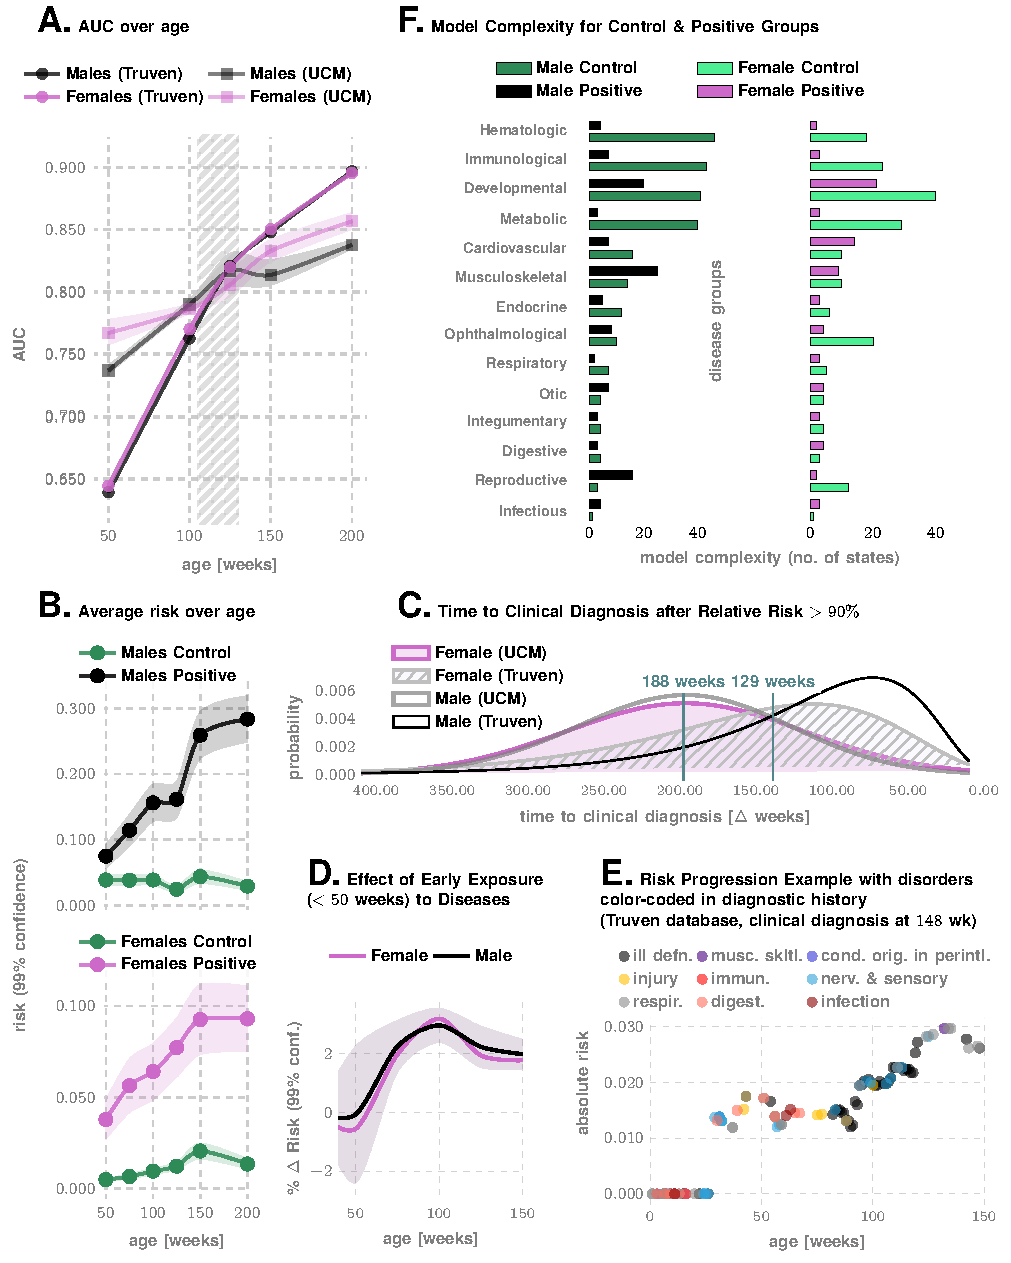
\includegraphics[width=0.99\textwidth]{Figures/External/main-figure1.pdf}
  \fi
     \vspace{-5pt}

     \captionN{Predictive Performance. Panel %C shows the distribution of the AUC, and panel
       A shows the ROC curves for males and females. Panel B shows the feature importance inferred by our prediction pipeline. The detailed description of the features is given in Extended Data Table~\ref{EXT-tab0}. The most import feature is related to immunologic disorders, and we note that in addition to features related to individual disease categories, we also have the mean control likelihood (rank 3), which may be interpreted as the average likelihood of the diagnostic patterns correspond to the control category as opposed to the \treatment category. Panels C and D show the spatial variation in the achieved predictive performance at 150 weeks, measured by AUC, for males and females, respectively. Gray areas lack data on either positive or negative cases. These county-specific AUC plots show that the performance of the algorithm has  relatively weak geospatial dependence, which is important in the light of current uneven distribution of diagnostic resources.
     }\label{fig1}
\end{figure*}
\else
\refstepcounter{figure}\label{fig1}
\fi
%###########################################################
%###########################################################
%###########################################################
%###########################################################
\ifFIGS
\begin{figure*}[!ht]
  \tikzexternalenable
  \vspace{-15pt}
  
  \centering 
 \def\DATA{../../data_revision}
\iftikzX
  

\pgfplotsset{
    discard if/.style 2 args={
        x filter/.append code={
            \edef\tempa{\thisrow{#1}}
            \edef\tempb{#2}
            \ifx\tempa\tempb
                \def\pgfmathresult{inf}
            \fi
        }
    },
    discard if not/.style 2 args={
        x filter/.append code={
            \edef\tempa{\thisrow{#1}}
            \edef\tempb{#2}
            \ifx\tempa\tempb
            \else
                \def\pgfmathresult{inf}
            \fi
        }
    }
  }

  \begin{tikzpicture}[font=\bf\sffamily\fontsize{8}{10}\selectfont]
\def\TEXTCOL{gray}
    \tikzset{
        hatch distance/.store in=\hatchdistance,
        hatch distance=20pt,
        hatch thickness/.store in=\hatchthickness,
        hatch thickness=2pt
    }

%     \makeatletter
%     \pgfdeclarepatternformonly[\hatchdistance,\hatchthickness]{flexible hatch}
%     {\pgfqpoint{0pt}{0pt}}
%     {\pgfqpoint{\hatchdistance}{\hatchdistance}}
%     {\pgfpoint{\hatchdistance-1pt}{\hatchdistance-1pt}}%
%     {
%         \pgfsetcolor{\tikz@pattern@color}
%         \pgfsetlinewidth{\hatchthickness}
%         \pgfpathmoveto{\pgfqpoint{0pt}{0pt}}
%         \pgfpathlineto{\pgfqpoint{\hatchdistance}{\hatchdistance}}
%         \pgfusepath{stroke}
%     }
%     \makeatother
% \pgfdeclarepatternformonly{north east lines wide}%
%    {\pgfqpoint{-1pt}{-1pt}}%
%    {\pgfqpoint{10pt}{10pt}}%
%    {\pgfqpoint{9pt}{9pt}}%
%    {
%      \pgfsetlinewidth{0.4pt}
%      \pgfpathmoveto{\pgfqpoint{0pt}{0pt}}
%      \pgfpathlineto{\pgfqpoint{9.1pt}{9.1pt}}
%      \pgfusepath{stroke}
%     }


  \def\WDT{4.75in} 
  \def\WDTA{2in} 

  \def\datafile{../../data_latest/figfiles/model_complexity.csv}
  \def\riskfile{\DATA/figfiles/risk.csv}
  \def\sampleimg{\DATA/figfiles/sample.pdf}
  \def\sampledat{\DATA/figfiles/sampledat.csv}
  \def\auctime{\DATA/figfiles/auc_time.csv}
  \def\auctimeV{\DATA/figfiles/Vauc_time.csv}
  \def\randomsamples{\DATA/figfiles/cfbd_auctime.csv}

  
  \def\horzm{../../perturbation_browser/ntb/male_horizon.csv}
  \def\horzmt{../../perturbation_browser/ntb/male_horizon_T.csv}
 \def\horzf{../../perturbation_browser/ntb/female_horizon.csv}
  \def\horzft{../../perturbation_browser/ntb/female_horizon_T.csv}
  \def\perturbneg{../../perturbation_browser/ntb/perturb_neg.csv}
  \def\track{../../perturbation_browser/ntb/track.csv}

  \def\PNEGA{A020571551}
  \def\PNEGB{A005421148}
  \def\PNEGC{A033768823}
  \def\PPOSA{A006621658}
  \def\PPOSB{A002483419}
  \def\PPOSC{A069615715}

  \def\HGT{1.6in}
  \def\WDT{3.5in}
  \def\WDTC{4in}
  \def\WDTR{1.9in}
  \def\WDTH{1.70in}

  \def\AXISCOL{white}
\def\BANDCOL{lightgray}
\def\PLOTCOLA{black}
\def\PLOTCOLB{\MXCOL}
\def\PLOTCOLBu{\MXCOL}
\def\PLOTCOLC{black}
\def\PLOTCOLD{\FXCOL}
\def\FNCOLB{SeaGreen2}
\def\PLOTCOLDu{\FXCOL}
\def\WDTa{1.85in}
\def\HGTa{2.6in}
\def\HGTaa{3.3in}
\def\WDTb{1in}
\def\HGTb{1.575in}

\def\SCALE{1.5}
\def\SCALEA{1.15}
\def\SCALEB{1.15}
\def\OPC{.75}
\def\OPCB{.85}
\def\BWIDTH{4pt}
\def\LWDT{0.5mm}
  \node[] (A0) at (0,0) {};

  \node[anchor=center] (N) at ([yshift=1in]A0.south)
  {
    \begin{tikzpicture}
       \begin{axis} [,legend cell align={left},
      legend style={anchor=east,at={(0,1.05)},
        inner sep=3pt,
        draw=none,
        fill=white,fill opacity=.85,
        align=left,anchor=west,
        text opacity=1,
        font=\bf\sffamily\fontsize{8}{9}\selectfont,text=black},
      grid style={thick,dashed, gray!40},
      grid,
    enlargelimits=true,scale only axis=true,scaled x ticks = false,scaled y ticks = false,
     height=\HGTa,
    width=\WDTa,
    enlarge x limits=0.07,axis line style={\AXISCOL, opacity=1,ultra  thick, rounded corners=0pt}, y tick label style={/pgf/number format/fixed,/pgf/number format/precision=3,/pgf/number format/fixed zerofill,
     /pgf/number format/1000 sep = %\thinspace % Optional if you want to replace comma as the 1000 separator 
      },
      major tick length=0pt,legend columns=2, legend style={,xshift=-.5in,yshift=.2in},
      yshift=-.75in,text=\TEXTCOL,xlabel={age [weeks]},xlabel style={yshift=0.025in},ylabel
      style={xshift=-0.1in},ylabel={AUC},
      grid style={thick,dashed, gray!40},
      ymax=0.9]

      
    \addplot[forget plot,smooth, draw=none,,name path=AA]table[col sep=comma,x=week, y=ub, discard if not={gender}{M}, discard if not={dataset}{UCM}]
    {\randomsamples};
    \addplot[forget plot,smooth,  draw=none,,name path=BB]table[col sep=comma,x=week, y=lb, discard if not={gender}{M}, discard if not={dataset}{UCM}]
    {\randomsamples};
    \addplot[forget plot,\MXCOL,opacity=.175] fill between[of=AA and BB];
    
      
    \addplot[forget plot,smooth, draw=none,,name path=AA]table[col sep=comma,x=week, y=ub, discard if not={gender}{F}, discard if not={dataset}{UCM}]
    {\randomsamples};
    \addplot[forget plot,smooth,  draw=none,,name path=BB]table[col sep=comma,x=week, y=lb, discard if not={gender}{F}, discard if not={dataset}{UCM}]
    {\randomsamples};
    \addplot[forget plot,\FXCOL,opacity=.175] fill between[of=AA and BB];
    
    
 \addplot[forget plot,smooth, draw=none,,name path=AA]table[col sep=comma,x=week, y=ub, discard if not={gender}{F}, discard if not={dataset}{Truven}]
    {\randomsamples};
    \addplot[forget plot,smooth,  draw=none,,name path=BB]table[col sep=comma,x=week, y=lb, discard if not={gender}{F}, discard if not={dataset}{Truven}]
    {\randomsamples};
    \addplot[forget plot,\MNCOL,opacity=.175] fill between[of=AA and BB];
    

    
 \addplot[forget plot,smooth, draw=none,,name path=AA]table[col sep=comma,x=week, y=ub, discard if not={gender}{M}, discard if not={dataset}{Truven}]
    {\randomsamples};
    \addplot[forget plot,smooth,  draw=none,,name path=BB]table[col sep=comma,x=week, y=lb, discard if not={gender}{M}, discard if not={dataset}{Truven}]
    {\randomsamples};
    \addplot[forget plot,\FNCOL,opacity=.1750] fill between[of=AA and BB];
    

      \end{axis}

   \begin{axis} [,legend cell align={left},
      legend style={anchor=east,at={(0,1.05)},
        inner sep=3pt,
        draw=none,
        fill=white,fill opacity=.85,
        align=left,anchor=west,
        text opacity=1,
        font=\bf\sffamily\fontsize{8}{9}\selectfont,text=black},
      grid style={thick,dashed, gray!40},
      grid,
    enlargelimits=true,scale only axis=true,scaled x ticks = false,scaled y ticks = false,
     height=\HGTa,
    width=\WDTa,
    enlarge x limits=0.07,axis line style={\AXISCOL, opacity=1,ultra  thick, rounded corners=0pt}, y tick label style={/pgf/number format/fixed,/pgf/number format/precision=3,/pgf/number format/fixed zerofill,
     /pgf/number format/1000 sep = %\thinspace % Optional if you want to replace comma as the 1000 separator 
      },
      major tick length=0pt,legend columns=2, legend style={,xshift=-.5in,yshift=.2in},
      yshift=-.75in,text=\TEXTCOL,xlabel={age [weeks]},xlabel style={yshift=0.025in},ylabel
      style={xshift=-0.1in},ylabel={AUC},
      grid style={thick,dashed, gray!40},
      ymax=0.9]
      
        \draw [draw=none,ultra thick,opacity=.3,postaction={
         pattern=flexible hatch,
        hatch distance=7pt,
        hatch thickness=2pt,
        draw=none,
        opacity=.5,
        pattern color=lightgray, %ultra thick,
     },] (axis cs:130,\pgfkeysvalueof{/pgfplots/ymin}) -- (axis cs:130,\pgfkeysvalueof{/pgfplots/ymax}) -- (axis cs:105,\pgfkeysvalueof{/pgfplots/ymax}) -- (axis cs:105,\pgfkeysvalueof{/pgfplots/ymin}) --cycle;

    \addplot[ smooth,  line width=\LWDT, \PLOTCOLB,mark=*, opacity=\OPC,
    mark options={%
      scale=\SCALEB,draw=\PLOTCOLB,  thick, fill=\PLOTCOLB,  opacity=\OPC,
    },]table[col sep=comma,x=week, y=v, discard if not={gender}{M}, discard if not={dataset}{Truven}]
    {\randomsamples};
    \addlegendentry{Males (Truven)}


    %
    \addplot[ smooth,  line width=\LWDT, \PLOTCOLBu,mark=square*, opacity=.5,
    mark options={%
      scale=\SCALEA,draw=\PLOTCOLBu,  thick, fill=\PLOTCOLBu,  opacity=.5,
    },]table[col sep=comma,x=week, y=v, discard if not={gender}{M}, discard if not={dataset}{UCM}]    {\randomsamples};
    \addlegendentry{Males (UCM)}





    
    \addplot[ smooth,  line width=\LWDT, \PLOTCOLD,mark=*, opacity=\OPCB,
    mark options={%
      scale=\SCALEB,draw=\PLOTCOLD,  thick, fill=\PLOTCOLD,  opacity=\OPCB,
    },]table[col sep=comma,x=week, y=v, discard if not={gender}{F}, discard if not={dataset}{Truven}]    {\randomsamples};
    \addlegendentry{Females (Truven)}
%
%
    \addplot[ smooth,  line width=\LWDT, \PLOTCOLDu,mark=square*, opacity=.5,
    mark options={%
      scale=\SCALEA,draw=\PLOTCOLDu,  thick, fill=\PLOTCOLDu,  opacity=.5,
    },]table[col sep=comma,x=week, y=v, discard if not={gender}{F}, discard if not={dataset}{UCM}]    {\randomsamples};
    \addlegendentry{Females (UCM)}



    

  \end{axis}



\end{tikzpicture}
  };

  
  \node[anchor=north west] (A) at ([xshift=0in,yshift=-.2in]N.north east) {
    \begin{tikzpicture}[anchor=center]
  \begin{groupplot}[group style={group name=A,group size= 2 by 1,horizontal sep=.5in},legend style={anchor=east,at={(.5,1.1)},/tikz/every even column/.append style={column sep=1.5in},legend cell align={left},inner sep=3pt,draw=none,fill=white,fill opacity=.85,align=right,text opacity=1,font=\bf\sffamily\fontsize{8}{9}\selectfont},axis line style={lightgray, opacity=0, thin},%
    enlargelimits=true,
     width=\HGT,
    height=\HGTaa,
     enlarge y limits=0.03,
    ] 
    \nextgroupplot[xbar,bar width=\BWIDTH,    
ytick=data,% crucial line for the xticklabels directive 
    ymin=0, 
    yticklabels from table={\datafile}{feature},
    yticklabel style={font=\bf\sffamily\fontsize{7}{7}\selectfont,align=right,rotate=0, 
text width=1.1in, anchor=east, yshift=0in,xshift=-.045in,text=\TEXTCOL},
    major tick length=0pt,
    yticklabel style={font=\bf\sffamily\fontsize{7}{7}\selectfont,text=\TEXTCOL},
    %grid,
    grid style={lightgray, opacity=.7},
    axis on top=false, 
    xlabel={},
    ylabel style={yshift=-1.25in,text=\TEXTCOL},,ylabel style={yshift=-.15in},
    ylabel={disease groups}]
    \addplot[opacity=1,fill=\MNCOL, area legend] table [ 
    y expr=\coordindex,
    x=NEGM
    ] {\datafile};   
    \addlegendentry{Male Control}
    \addplot[opacity=1,fill=\MXCOL, area legend] table [ 
    y expr=\coordindex,
    x=POSM
    ] {\datafile};   
    \addlegendentry{Male Positive}

    \nextgroupplot[xbar,bar width=\BWIDTH,    ytick=data,% crucial line for the xticklabels directive 
    ymin=0, 
    yticklabels from table={\datafile}{feature},
    yticklabel style={font=\bf\sffamily\fontsize{7}{7}\selectfont,align=right,rotate=0, 
text width=1.1in, anchor=east, yshift=0in,xshift=-.045in,text=\TEXTCOL},
    major tick length=0pt,
    yticklabel style={font=\bf\sffamily\fontsize{7}{7}\selectfont,text=\TEXTCOL},
    %grid,
    grid style={lightgray, opacity=.7},
    axis on top=false, 
    xlabel={model complexity (no. of states)},
    ylabel style={yshift=-0.69in,text=\TEXTCOL},yticklabels=\empty,xlabel style={text=\TEXTCOL,xshift=-.7in,yshift=.05in},]
    \addplot[opacity=1,fill=\FNCOLB, area legend] table [ 
    y expr=\coordindex,
    x=NEGF
    ] {\datafile};   
    \addlegendentry{Female Control}
    \addplot[opacity=1,fill=\FXCOL, area legend] table [ 
    y expr=\coordindex,
    x=POSF
    ] {\datafile};   
    \addlegendentry{Female Positive}
  \end{groupplot}
\end{tikzpicture}
};




\node[anchor=north west] (B) at ([yshift=-.275in]N.south west)
{
  \begin{tikzpicture}[]
    \begin{groupplot}[group style={group name=A,group size= 1 by 2, vertical sep=.35in},legend cell align={left},
      legend style={anchor=east,at={(-.2,1.05)},
        inner sep=3pt,
        draw=none,
        fill=white,fill opacity=.85,
        align=left,anchor=west,
        text opacity=1,
        font=\bf\sffamily\fontsize{8}{9}\selectfont,text=black},
      grid style={thick,dashed, gray!40},
      grid,
    enlargelimits=true,scale only axis=true,scaled x ticks = false,scaled y ticks = false,
     height=\HGTb,
    width=\WDTb,
    enlarge x limits=0.03,axis line style={\AXISCOL, opacity=1,ultra  thick, rounded corners=0pt}, y tick label style={/pgf/number format/fixed,/pgf/number format/precision=3,/pgf/number format/fixed zerofill,
     /pgf/number format/1000 sep = %\thinspace % Optional if you want to replace comma as the 1000 separator 
      },
      major tick length=0pt]

    \nextgroupplot[xticklabels=\empty,text=\TEXTCOL]
    \addplot[ smooth,  line width=\LWDT, \MNCOL,mark=*, opacity=.85,
    mark options={%
      scale=\SCALE,draw=\MNCOL,  thick, fill=\MNCOL,  opacity=1,
    },]table[col sep=comma,x=time, y=mcontrolM]
    {\riskfile};
    \addlegendentry{Males Control};
 

   \addplot[forget plot,smooth, draw=none,,name path=AA]table[col sep=comma,x=time, y=UcontrolM]
    {\riskfile};
    \addplot[forget plot,smooth,  draw=none,,name path=BB]table[col sep=comma,x=time, y=LcontrolM]
    {\riskfile};
    \addplot[forget plot,\MNCOL,opacity=.175] fill between[of=AA and BB];
    

    
    \addplot[ smooth,  line width=\LWDT, \MXCOL,mark=*, opacity=.85,
    mark options={%
      scale=\SCALE,draw=\MXCOL,  thick, fill=\MXCOL,  opacity=1,
    },]table[col sep=comma,x=time, y=mtreatmentM]
    {\riskfile};
    \addlegendentry{Males Positive};


    
   \addplot[smooth, draw=none,,name path=A]table[col sep=comma,x=time, y=UtreatmentM]
    {\riskfile};
    \addplot[smooth,  draw=none,,name path=B]table[col sep=comma,x=time, y=LtreatmentM]
    {\riskfile};
    \addplot[\MXCOL,opacity=.175] fill between[of=A and B];
    

    \nextgroupplot[xlabel={age [weeks]},text=\TEXTCOL,xlabel style={yshift=0.025in},,ylabel={risk (99\% confidence)},ylabel style={xshift=.3in,yshift=.15in}]
    \addplot[ smooth, line width=\LWDT, \FNCOL,mark=*, opacity=.85,
    mark options={%
      scale=\SCALE,draw=\FNCOL,  thick, fill=\FNCOL,  opacity=1,
    },]table[col sep=comma,x=time, y=mcontrolF]
    {\riskfile};
    \addlegendentry{Females Control};

   \addplot[forget plot,smooth, draw=none,,name path=Ax,]table[col sep=comma,x=time, y=UcontrolF]
    {\riskfile};
    \addplot[forget plot,smooth, draw=none,,name path=Bx]table[col sep=comma,x=time, y=LcontrolF]
    {\riskfile};
    \addplot[forget plot,\FNCOL,opacity=.175] fill between[of=Ax and Bx];
    

    
    \addplot[ smooth,  line width=\LWDT, \PLOTCOLD,mark=*, opacity=.85,
    mark options={%
      scale=\SCALE,draw=\PLOTCOLD,  thick, fill=\PLOTCOLD,  opacity=1,
    },]table[col sep=comma,x=time, y=mtreatmentF]
    {\riskfile};
    \addlegendentry{Females Positive};

   \addplot[smooth, draw=none,,name path=A]table[col sep=comma,x=time, y=UtreatmentF]
    {\riskfile};
    \addplot[smooth,  draw=none,,name path=B]table[col sep=comma,x=time, y=LtreatmentF]
    {\riskfile};
    \addplot[\PLOTCOLD,opacity=.175] fill between[of=A and B];

\end{groupplot}


    \end{tikzpicture}
  };
%     ###########################################
%     ###########################################
%     ###########################################
  \def\WDTX{4.675in}
  \def\HGTX{1.35in}
  
  \node [anchor=north west] (D) at (B.north east)
  {
    \begin{tikzpicture}
      \begin{axis}[legend cell align=left,legend style={anchor=east,at={(0.35,.85)},
          inner sep=3pt,draw=none,fill=none,fill opacity=.85,
          align=right,text opacity=1,
          font=\bf\sffamily\fontsize{8}{9}\selectfont},,axis line style={lightgray, opacity=0, thin},%
        height=\HGTX, width=\WDTX,
        %ybar,bar width=4pt,    
        major tick length=0.0pt,
        ylabel={probability},
        %xmin=100,
        %xmax=0.35,
        xticklabel style={font=\bf\sffamily\fontsize{7}{7}\selectfont,text=\TEXTCOL},
        %grid,
        grid style={lightgray, dashed,opacity=.7},
        axis on top=false, 
        xlabel={time to clinical diagnosis [$\Delta$ weeks]}, x tick label style={yshift=0.05in,text=\TEXTCOL},
        xlabel style={yshift=0.05in,text=\TEXTCOL},ylabel style={yshift=0.05in,xshift=-.4in,text=\TEXTCOL},x tick label style={,text=\TEXTCOL,xshift=.1in,yshift=-.05in,/pgf/number format/fixed,/pgf/number format/precision=2,/pgf/number format/fixed zerofill,
          /pgf/number format/1000 sep = %\thinspace
        },y tick label style={text=\TEXTCOL,/pgf/number format/fixed,/pgf/number format/precision=3,/pgf/number format/fixed zerofill,
          /pgf/number format/1000 sep = %\thinspace 
        },scaled ticks=false, enlarge y limits=0.07,enlarge x limits=0,x dir=reverse
        ]
\def\OPC{.2}
     \addplot[smooth, ultra thick, fill=\FXCOL, fill opacity=\OPC,draw=\FXCOL,area legend,,name path=A]table[col sep=comma,x=x, y=pdf]
    {\horzf};
          \addlegendentry{Female (UCM)}
   \addplot[smooth, draw=lightgray, very thick, fill=Lavender, fill opacity=\OPC,,,name path=A,area legend,postaction={
         pattern=flexible hatch,
        hatch distance=7pt,
        hatch thickness=1pt,
        draw=none,
        opacity=1,
        pattern color=lightgray, %ultra thick,
     },]table[col sep=comma,x=x, y=pdf]
    {\horzft};
    \addlegendentry{Female (Truven)}
    %
    \addplot[smooth, draw=gray,ultra thick, opacity=0.7,fill=none,area legend, fill opacity=\OPC,,name path=A]table[col sep=comma,x=x, y=pdf]
    {\horzm};
    \addlegendentry{Male (UCM)}
    %
    \addplot[smooth, draw=black,  thick, fill=none, fill opacity=\OPC,,area legend,,name path=A]table[col sep=comma,x=x, y=pdf]
    {\horzmt};
    \addlegendentry{Male (Truven)}

     \draw [CadetBlue4,,semithick] (axis cs:129,\pgfkeysvalueof{/pgfplots/ymin}) -- (axis cs:129,\pgfkeysvalueof{/pgfplots/ymax}) node [pos=1.0,,above,yshift=-0.15in,xshift=-.0in,fill=white] {129 weeks};
     \draw [CadetBlue4,,semithick] (axis cs:188,\pgfkeysvalueof{/pgfplots/ymin}) -- (axis cs:188,\pgfkeysvalueof{/pgfplots/ymax}) node [pos=1.0,,above,yshift=-0.15in,xshift=-.0in,fill=white] {188 weeks};
       \end{axis}
      \end{tikzpicture}
    };
 

      \node [anchor=north west] (E) at ([xshift=0in,yshift=-.62in]D.south west)
  {
    \begin{tikzpicture}
      \begin{axis}[legend cell align=left, legend columns=2,     legend style={,anchor=east,at={(1,1.2)},
          inner sep=3pt,draw=none,fill=white,fill opacity=.85,
          align=right,text opacity=1,
          font=\bf\sffamily\fontsize{8}{9}\selectfont},,axis line style={lightgray, opacity=0, thin},%
        height=1.95in,
        width=1.85in,
        %ybar,bar width=4pt,    
        major tick length=0.0pt,
        ylabel={\% $\Delta$ Risk (99\% conf.)},
        xmin=40,
        %xmax=0.35,
        xticklabel style={font=\bf\sffamily\fontsize{7}{7}\selectfont,text=\TEXTCOL},
        grid,
        grid style={lightgray, dashed,opacity=.7},
        axis on top=false, 
        xlabel={age [weeks]}, x tick label style={yshift=0.0in,text=\TEXTCOL},
        xlabel style={yshift=0.0in,text=\TEXTCOL},ylabel style={yshift=-0.1in,xshift=-.7in,text=\TEXTCOL},x tick label style={,text=\TEXTCOL,xshift=.1in,yshift=-.05in,/pgf/number format/fixed,/pgf/number format/precision=2,/pgf/number format/fixed zerofill,
          /pgf/number format/1000 sep = %\thinspace
        },y tick label style={text=\TEXTCOL,/pgf/number format/fixed,/pgf/number format/precision=0,/pgf/number format/fixed zerofill,
          /pgf/number format/1000 sep = %\thinspace 
        },x tick label style={xshift=-.1in,text=\TEXTCOL,/pgf/number format/fixed,/pgf/number format/precision=0,/pgf/number format/fixed zerofill,
          /pgf/number format/1000 sep = %\thinspace 
        },scaled ticks=false, enlarge y limits=0.07,enlarge x limits=0,
        ]
\def\OPC{.2}
     \addplot[smooth, ultra thick,draw=\FXCOL,,name path=A]table[col sep=comma,x=week, y=MEDIANF]
    {\perturbneg};
          \addlegendentry{Female}
     \addplot[smooth, ultra thick,draw=\MXCOL,,name path=A]table[col sep=comma,x=week, y=MEDIANM]
    {\perturbneg};
    \addlegendentry{Male}

     \addplot[forget plot,smooth, ultra thick,draw=none,,name path=A]table[col sep=comma,x=week, y=UBM]
    {\perturbneg};
      \addplot[forget plot,smooth, ultra thick,draw=none,,name path=B]table[col sep=comma,x=week, y=LBM]
      {\perturbneg};
          \addplot[forget plot,\FXCOL,opacity=.085] fill between[of=A and B];
   \addplot[forget plot,smooth, ultra thick,draw=none,,name path=A]table[col sep=comma,x=week, y=UBF]
    {\perturbneg};
      \addplot[forget plot,smooth, ultra thick,draw=none,,name path=B]table[col sep=comma,x=week, y=LBF]
      {\perturbneg};
          \addplot[forget plot,\MXCOL,opacity=.085] fill between[of=A and B];

       \end{axis}
      \end{tikzpicture}
    };
\definecolor{alizarin}{rgb}{0.82, 0.1, 0.26}
\definecolor{amber}{rgb}{1.0, 0.75, 0.0}
\definecolor{amethyst}{rgb}{0.6, 0.4, 0.8}
\definecolor{apricot}{rgb}{0.98, 0.81, 0.69}
\definecolor{atomictangerine}{rgb}{1.0, 0.6, 0.4}
\definecolor{awesome}{rgb}{1.0, 0.13, 0.32}
\definecolor{azurec}{rgb}{0.0, 0.5, 1.0}
\definecolor{ballblue}{rgb}{0.13, 0.67, 0.8}
\definecolor{bittersweet}{rgb}{1.0, 0.44, 0.37}
\definecolor{bluem}{rgb}{0.0, 0.5, 0.69}
\definecolor{brightturquoise}{rgb}{0.03, 0.91, 0.87}
\definecolor{fiveA}{HTML}{30a2da}
\definecolor{fiveB}{HTML}{fc4f30}
\definecolor{fiveC}{HTML}{e5ae38}
\definecolor{fiveD}{HTML}{6d904f}
\definecolor{fiveE}{HTML}{8b8b8b}

\def\CINF{Red4}
\def\CNEO{SeaGreen4}
\def\CIMM{Red1}
\def\CBLD{lightgray}
\def\CNRV{fiveA}
\def\CCIR{Green2}
\def\CRSP{fiveE}
\def\CDIG{bittersweet}
\def\CSKN{Cyan3}
\def\CMSK{Indigo}
\def\CCNT{Orchid3}
\def\CPRI{MediumBlue!80}
\def\CINJ{amber}
\def\CMNT{DarkGreen!90}
\def\CGNT{DarkOrange3}
\def\CILL{black}
\def\HCOL{black}
\def\HBLK{gray}
\def\SCALEB{1.2}
\def\OPC{.6}
\def\SCALER{0.01}
\node [anchor=north west] (F) at ([xshift=0.1in,yshift=0in]E.north east)
  {
    \begin{tikzpicture}
      \begin{axis}[legend cell align=left, legend columns=3,     legend style={,anchor=east,at={(1.05,1.2)},
          inner sep=3pt,draw=none,fill=white,fill opacity=.85,
          align=right,text opacity=1,text=\TEXTCOL,
          font=\bf\sffamily\fontsize{8}{9}\selectfont},,axis line style={lightgray, opacity=0, thin},%
        height=1.88in,
        width=2.85in,
        %ybar,bar width=4pt,    
        major tick length=0.0pt,
        ylabel={absolute risk},
        xmin=0,
        xmax=150,
        xticklabel style={font=\bf\sffamily\fontsize{7}{7}\selectfont,text=\TEXTCOL},
        grid,
        grid style={lightgray, dashed,opacity=.7},
        axis on top=false, 
        xlabel={age [weeks]}, x tick label style={yshift=0.05in,text=\TEXTCOL},
        xlabel style={yshift=0.05in,text=\TEXTCOL},ylabel style={yshift=0.05in,xshift=-0.2in,text=\TEXTCOL},x tick label style={,text=\TEXTCOL,xshift=.1in,yshift=-.05in,/pgf/number format/fixed,/pgf/number format/precision=2,/pgf/number format/fixed zerofill,
          /pgf/number format/1000 sep = %\thinspace
        },y tick label style={text=\TEXTCOL,/pgf/number format/fixed,/pgf/number format/precision=3,/pgf/number format/fixed zerofill,
          /pgf/number format/1000 sep = %\thinspace 
        },,x tick label style={xshift=-.1in,text=\TEXTCOL,/pgf/number format/fixed,/pgf/number format/precision=0,/pgf/number format/fixed zerofill,
          /pgf/number format/1000 sep = %\thinspace 
        },scaled ticks=false, enlarge y limits=0.07,enlarge x limits=0,
        ]
        \addplot[forget plot,smooth,draw=black,ultra thick, line width = 5pt,opacity=0 , mark=none,  mark options={%
       scale=\SCALEB,
       opacity=0.05,
     }]table[col sep=comma,y expr=\thisrowno{1}*\SCALER, x=week]
    {\track};
%
        \addplot[,only marks, mark=*,  mark options={%
       scale=\SCALEB,fill=\CILL,draw=\CILL,
       opacity=\OPC,
     }]table[col sep=comma,y expr=\thisrowno{1}*\SCALER, x=week,discard if not={icdclass}{15.0}]
     {\track};
     \addlegendentry{ill defn.}
%
 %
        \addplot[,only marks, mark=*,  mark options={%
       scale=\SCALEB,fill=\CMSK,draw=\CMSK,
       opacity=\OPC,
     }]table[col sep=comma,y expr=\thisrowno{1}*\SCALER, x=week,discard if not={icdclass}{12.0}]
    {\track};
     \addlegendentry{musc. skltl.}
%
%
        \addplot[,only marks, mark=*,  mark options={%
       scale=\SCALEB,fill=\CPRI,,draw=\CPRI,
       opacity=\OPC,
     }]table[col sep=comma,y expr=\thisrowno{1}*\SCALER, x=week,discard if not={icdclass}{14.0}]
    {\track};
     \addlegendentry{cond. orig. in perintl.}
%
        \addplot[,only marks, mark=*,  mark options={%
       scale=\SCALEB,fill=\CINJ,draw=\CINJ,
       opacity=\OPC,
     }]table[col sep=comma,y expr=\thisrowno{1}*\SCALER, x=week,discard if not={icdclass}{16.0}]
    {\track};
     \addlegendentry{injury}
%
%
        \addplot[,only marks, mark=*,  mark options={%
       scale=\SCALEB,fill=\CIMM,draw=\CIMM,
       opacity=\OPC,
     }]table[col sep=comma,y expr=\thisrowno{1}*\SCALER, x=week,discard if not={icdclass}{2.0}]
    {\track};
     \addlegendentry{immun.}
%
%
        \addplot[,only marks, mark=*,  mark options={%
       scale=\SCALEB,fill=\CNRV,draw=\CNRV,
       opacity=\OPC,
     }]table[col sep=comma,y expr=\thisrowno{1}*\SCALER, x=week,discard if not={icdclass}{5.0}]
    {\track};
     \addlegendentry{nerv. \& sensory}
%
%
        \addplot[,only marks, mark=*,  mark options={%
       scale=\SCALEB,fill=\CRSP,draw=\CRSP,
       opacity=\OPC,
     }]table[col sep=comma,y expr=\thisrowno{1}*\SCALER, x=week,discard if not={icdclass}{7.0}]
    {\track};
     \addlegendentry{respir.}
%
       \addplot[,only marks, mark=*,  mark options={%
       scale=\SCALEB,fill=\CDIG,draw=\CDIG,
       opacity=\OPC,
     }]table[col sep=comma,y expr=\thisrowno{1}*\SCALER, x=week,discard if not={icdclass}{8.0}]
    {\track};
     \addlegendentry{digest.}
       \addplot[,only marks, mark=*,  mark options={%
       scale=\SCALEB,fill=\CINF,draw=\CINF,
       opacity=\OPC,
     }]table[col sep=comma,y expr=\thisrowno{1}*\SCALER, x=week,discard if not={icdclass}{0.0}]
    {\track};
     \addlegendentry{infection}
    % 
  \end{axis}
      \end{tikzpicture}
    };





   \node[anchor=south west,align=left] (LA) at ([xshift=.2in,yshift=-.2in]N.north west) {{\LARGE A.} AUC over age  };
   \node[anchor=north west,align=left] (LB) at ($(LA.north west)!(A.north west)!(LA.north east)$) {{\LARGE F.} Model Complexity for Control \& Positive Groups  };
  \node[anchor=south west,align=left] (LB1) at ($(LA.north west)!(B.north west)!(LA.south west)$) {{\LARGE B.} Average risk over age   };
  \node[anchor=south west,align=left] (LB2) at ($(LB1.south west)!(LB.west)!(LB1.south east)$) {{\LARGE C.} Time to Clinical Diagnosis after Relative Risk $> 90\%$   };
  \node[anchor=south west,align=left] (LB3) at ([xshift=-.6in,yshift=.1in]$(LB2.south west)!(E.north west)!(LB2.north west)$) {{\LARGE D.} Effect of Early Exposure \\($<50$ weeks)  to  Diseases  };

 \node[anchor=north west,align=left] (LB3) at ([xshift=0.2in]$(LB3.north west)!(F.north west)!(LB3.north east)$) {{\LARGE E.} Risk Progression Example with disorders\\color-coded  in diagnostic history\\(Truven database, clinical diagnosis at $148$ wk) };


  % \node[anchor=north west,align=left] (LD) at ($(LA.north west)!(LB1.north)!(LA.south west)$) {{\LARGE C.} Risks for 6 Random Subjects};

\end{tikzpicture}


  \else
   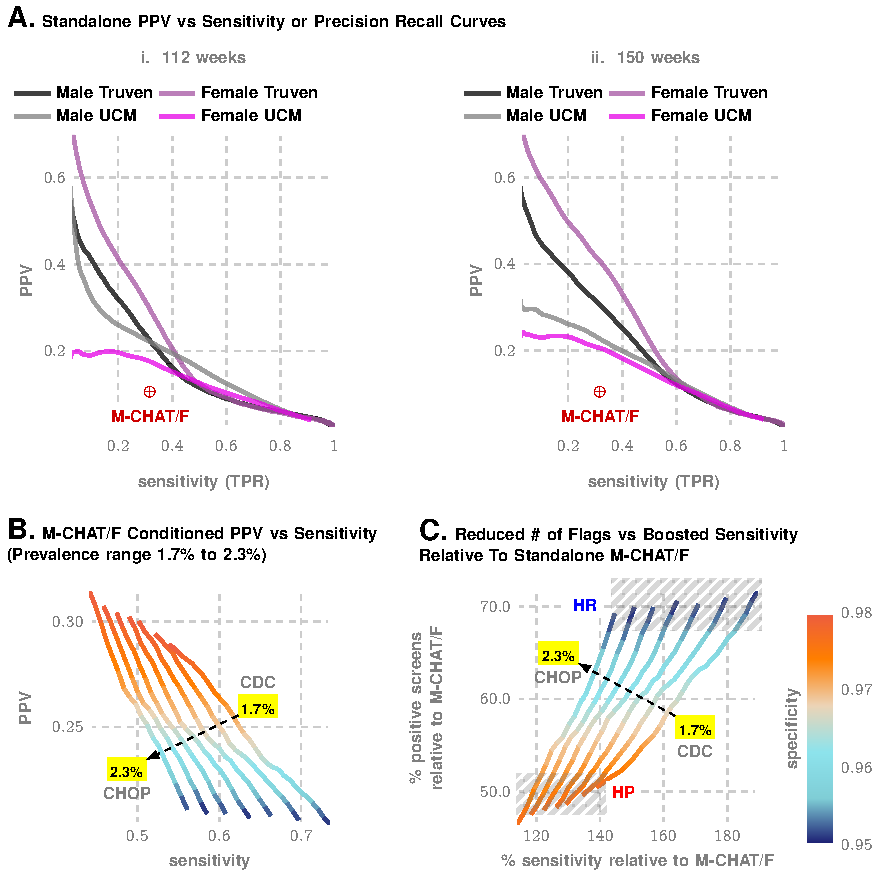
\includegraphics[width=0.99\textwidth]{Figures/External/main-figure2.pdf}
   \fi
   \vspace{-10pt}

    \captionN{\textbf{More details on Predictive Performance and Variation of Inferred Risk.} Panel A illustrates AUC achieved as a function of
      patient age, for the Truven and UCM datasets. The shaded area outlines the 2 - 2.5  years of age, and  shows that we achieve $>80\%$ AUC for either gender from shortly after 2 years.   Panel B illustrates how the average risk changes with time for the control and the positive cohorts. Panel C shows the distribution of the prediction horizon: the time to a clinical diagnosis after inferred  relative risk crosses $90\%$. Panel D shows that for each new disease code for a low-risk child, ASD risk increases by approximately $2\%$ for either gender. Panel E illustrates the risk progression of a specific, ultimately autistic male child in the Truven database. Abbreviations in the legend: ill defn. (Symptoms, Signs, And Ill-Defined Conditions),   musc. skltl. (Diseases Of The Musculoskeletal System And Connective Tissue), cond. orig. in perintl. (Certain Conditions Originating In The Perinatal Period), immun. (Endocrine, Nutritional And Metabolic Diseases, And Immunity Disorders), nerv. \& sensory (Diseases Of The Nervous System And Sense Organs), respir. (Respiratory Disorders), and digest. (Digestive Disorders). Panel F illustrates  how inferred models differ between the control vs. the \treatment cohorts. On average, models get less complex, implying the exposures get more statistically independent.}\label{fig2}
\end{figure*}
\else
\refstepcounter{figure}\label{fig2}
\fi
%###########################################################
%###########################################################
%###########################################################
\ifFIGS
%###########################################################
\begin{figure*}[t]
  \tikzexternalenable
  \vspace{-10pt}

  \centering
  
  \def\AXISCOL{white}
  \def\TEXTCOL{gray}
  \tikzset{
    hatch distance/.store in=\hatchdistance,
    hatch distance=20pt,
    hatch thickness/.store in=\hatchthickness,
    hatch thickness=2pt
  }
  \pgfplotsset{
    discard if/.style 2 args={
      x filter/.append code={
        \edef\tempa{\thisrow{#1}}
        \edef\tempb{#2}
        \ifx\tempa\tempb
        \def\pgfmathresult{inf}
        \fi
      }
    },
    discard if not/.style 2 args={
      x filter/.append code={
        \edef\tempa{\thisrow{#1}}
        \edef\tempb{#2}
        \ifx\tempa\tempb
        \else
        \def\pgfmathresult{inf}
        \fi
      }
    }
  }
  \begin{tikzpicture}[font=\bf\sffamily\fontsize{8}{10}\selectfont ]
    \def\DATAPATH{../../../revision_results/roc/restricted_neg_len/RAW/}
    \def\datafile{\DATAPATH/RAWPRCpipeline_BASIC_M_150w.csv}
    \def\datafileF{\DATAPATH/RAWPRCpipeline_BASIC_F_150w.csv}
    \def\datafileU{\DATAPATH/RAWPRCvalid_BASIC_M_150w.csv}
    \def\datafileUF{\DATAPATH/RAWPRCvalid_BASIC_F_150w.csv}

    \def\datafileh{\DATAPATH/RAWPRCpipeline_BASIC_M_112w.csv}
    \def\datafileFh{\DATAPATH/RAWPRCpipeline_BASIC_F_112w.csv}
    \def\datafileUh{\DATAPATH/RAWPRCvalid_BASIC_M_112w.csv}
    \def\datafileUFh{\DATAPATH/RAWPRCvalid_BASIC_F_112w.csv}

    \def\HGT{1.95in}
    \def\WDT{1.75in}
    \def\HGTa{1.55in}
    \def\WDTa{1.6in}

    \def\FXCOL{Orchid3!80!black}
    \def\MXCOLB{gray}
    \def\FXCOLB{Fuchsia!90!black}
    \def\OPC{.75}
    \def\LWDT{.6mm}
    \def\SKIP{7}

    \node[anchor=north east] (N) 
    {
      \begin{tikzpicture}[text=\TEXTCOL,]
        \begin{groupplot}
          [name=Agg,
          group style={
            group name=Ag,
            group size=2 by 1,
            % xlabels at=edge bottom,
            % xticklabels at=edge bottom,
            horizontal sep=1.25in,
            % horizontal sep=.55in,
          },        ,legend cell align={left},
          legend style={anchor=east,at={(-0.25,1.1)},
            inner sep=3pt,
            draw=none,
            fill=white,fill opacity=.850,
            align=left,anchor=west,
            text opacity=1,
            font=\bf\sffamily\fontsize{8}{9}\selectfont,text=black},
          legend columns=2, 
          name=K,
          clip=true,,
          width=\WDT,
          height=\HGT,
          scale only axis=true,
          enlargelimits=false,
          axis on top=false,
          % axis background/.style={
          % shade,top color=transparent!5,bottom color=transparent!5},
          axis line style={\AXISCOL, opacity=1,ultra  thick, 
            rounded corners=0pt}, 
          grid,
          grid style={thick,dashed, gray!40},
          xticklabel style={yshift=-.05in},
          xlabel style={yshift=-.075in,text=\TEXTCOL},
          ylabel style={align=center,,text=\TEXTCOL,anchor=center,
            yshift=-.175in},
          % tickpos=left,
          ytick align=outside,
          xtick align=outside,
          major tick length=0pt,
          scaled y ticks = false,
          y tick label style={/pgf/number format/fixed,
            /pgf/number format/1000 sep = \thinspace % Optional if you00 separator 
          },
          ylabel={PPV},xlabel={sensitivity (TPR)},
          title style={ yshift=.35in,xshift=-0.5in,anchor=south west,text=\TEXTCOL},
          % extra x ticks={1},extra x tick labels={1}
          ]

          \nextgroupplot[ , xmin=0.03, ymax=0.7,
          title={{ i. } 112 weeks},
          ]
          \addplot [each nth point=\SKIP, filter discard warning=false, 
          unbounded coords=discard,smooth,draw=\MXCOL, line width=\LWDT,opacity=\OPC,
          ]table [col sep=comma,x=tpr,y=p] {\datafileh};
          \addlegendentry{Male Truven}

          \addplot [each nth point=\SKIP, filter discard warning=false, 
          unbounded coords=discard,smooth,draw=\FXCOL,
          line width=\LWDT,,opacity=\OPC,
          ]table [col sep=comma,x=tpr,y=p] {\datafileFh};
          \addlegendentry{Female Truven}

          \addplot [each nth point=\SKIP, filter discard warning=false, 
          unbounded coords=discard,smooth,draw=\MXCOLB,
          line width=\LWDT,,opacity=\OPC,
          ]table [col sep=comma,x=tpr,y=p] {\datafileUh};
          \addlegendentry{Male UCM}

          \addplot [each nth point=\SKIP, filter discard warning=false, 
          unbounded coords=discard,smooth,draw=\FXCOLB,
          line width=\LWDT,,opacity=\OPC,
          ]table [col sep=comma,x=tpr,y=p] {\datafileUFh};
          \addlegendentry{Female UCM}

          \node[] (MC) at (axis cs:.388,.146) {};


          \nextgroupplot[ xlabel={sensitivity (TPR)},xmin=0.03,
          ymax=0.7,
          ,title={{ ii. } 150 weeks}
          ]
          \addplot [each nth point=\SKIP, filter discard warning=false, 
          unbounded coords=discard,smooth,draw=\MXCOL,
          line width=\LWDT,,opacity=\OPC,
          ]table [col sep=comma,x=tpr,y=p] {\datafile};
          \addlegendentry{Male Truven}

          \addplot [each nth point=\SKIP, filter discard warning=false, 
          unbounded coords=discard,smooth,draw=\FXCOL,
          line width=\LWDT,,opacity=\OPC,
          ]table [col sep=comma,x=tpr,y=p] {\datafileF};
          \addlegendentry{Female Truven}

          \addplot [each nth point=\SKIP, filter discard warning=false, 
          unbounded coords=discard,smooth,draw=\MXCOLB,
          line width=\LWDT,,opacity=\OPC,
          ]table [col sep=comma,x=tpr,y=p] {\datafileU};
          \addlegendentry{Male UCM}

          \addplot [each nth point=\SKIP, filter discard warning=false, 
          unbounded coords=discard,smooth,draw=\FXCOLB,
          line width=\LWDT,,opacity=\OPC,
          ]table [col sep=comma,x=tpr,y=p] {\datafileUF};
          \addlegendentry{Female UCM}
          \node[] (MC1) at (axis cs:.388,.146) {};

        \end{groupplot}
          \node[text=Red3,label={[fill=white,font=\bf\sffamily\fontsize{7}{7},text=Red3]-90:M-CHAT/F}] (MC1) at (MC1) {$\oplus$};
          \node[text=Red3,label={[fill=white,font=\bf\sffamily\fontsize{7}{7},text=Red3]-90:M-CHAT/F}] (MC) at (MC) {$\oplus$};

        
      \end{tikzpicture}
    };

    \node[anchor=north west] (N1) at ([yshift=-.45in]N.south west) {
      \def\datafile{../optcode_/data/spcrho.csv}
      \begin{tikzpicture}[text=\TEXTCOL, ]
        \begin{groupplot}
          [name=Agg,
          group style={
            group name=Ag,
            group size=2 by 1,
            xlabels at=edge bottom,
            xticklabels at=edge bottom,
            vertical sep=.75in,
            horizontal sep=1.25in,
          },        ,legend cell align={left},
          legend style={anchor=east,at={(-0.12,1.1)},
            inner sep=3pt,
            draw=none,
            fill=white,fill opacity=.850,
            align=left,anchor=west,
            text opacity=1,
            font=\bf\sffamily\fontsize{8}{9}\selectfont,text=black},
          legend columns=2, 
          name=K,
          clip=true,,
          width=\WDTa,
          height=\HGTa,
          scale only axis=true,
          enlargelimits=false,
          axis on top=false,
          axis line style={\AXISCOL, opacity=1,ultra  thick, 
            rounded corners=0pt}, 
          grid,
          grid style={thick,dashed, gray!40},
          % xticklabel style={xshift=0.05in,yshift=-.05in},
          xlabel style={yshift=.05in,text=\TEXTCOL},
          ylabel style={align=center,,text=\TEXTCOL,anchor=center,
            yshift=-.05in},,y tick label style={/pgf/number format/fixed,
            /pgf/number format/precision=2,/pgf/number format/fixed zerofill,
            /pgf/number format/1000 sep = %\thinspace % Optional if you want
          },
          % tickpos=left,
          ytick align=outside,
          xtick align=outside,
          major tick length=0pt,
          scaled y ticks = false,
          y tick label style={/pgf/number format/fixed,
            /pgf/number format/1000 sep = \thinspace % Optional if you00 separator 
          },
          ylabel={PPV},xlabel={sensitivity (TPR)},point meta=explicit,
          colorbar style={width=.1in,
            y tick label style={/pgf/number format/fixed,
              /pgf/number format/precision=2,
              /pgf/number format/fixed zerofill,
              /pgf/number format/1000 sep = %\thinspace % Optional if you want to replace comma as the 1000 separator 
            },}%,x tick label style={yshift=-.2in},xlabel style={yshift=-.2in},
          % extra x ticks={1},extra x tick labels={1}
          ]

          \nextgroupplot[%title={{\Large C.} PPV vs. sensitivity},
          % colorbar horizontal,
          extra y ticks={0.15},
          % ymin=0.15,xmin=0.39,
          % xmin=.98,extra x ticks={1},
          colorbar style={at={(0,1.1)},title={specificity},title style={yshift=-.1in},
            height=.1in,scaled x ticks=false,
            x tick label style={/pgf/number format/fixed,
              /pgf/number format/precision=3,/pgf/number format/fixed zerofill,
              /pgf/number format/1000 sep = %\thinspace % Optional to replace comma as the 1000 separator 
            },
            xticklabel style={yshift=-.025in},},ylabel={PPV},xlabel={sensitivity}]
          % \pgfplotsset{
          % colormap={hot}{color(0cm)=(lightgray!70); color(1cm)=(lightgray!80); color(2cm)=(lightgray!80!Bisque1); color(3cm)=(Bisque1!90!Tomato); color(4cm)=(Tomato); color(5cm)=(Red1)}
          % } 
          \pgfplotsset{
            colormap={hot}{color(0cm)=(MidnightBlue); color(1cm)=(CadetBlue2!90!black); color(2cm)=(CadetBlue1!93!black); color(3cm)=(Bisque1!93!black); color(4cm)=(DarkOrange1); color(5cm)=(Tomato!93!black)}
          }

          \addplot [mesh, each nth point=\SKIP, filter discard warning=false, 
          unbounded coords=discard,line width=\LWDT]table [col sep=comma,x expr=\thisrow{s},y expr=\thisrow{p},meta=c,
          % discard if not={gender}{M},
          restrict expr to domain={\thisrow{c}}{0.95:.977},
          restrict expr to domain={\thisrow{rho}}{0.017:0.024},
          % restrict expr to domain={\thisrow{s}}{1:1.5},
          ] {\datafile};   

          \node[anchor=west] (r1) at (axis cs:.48,0.23) {};
          \node[anchor=west] (r2) at (axis cs:0.64,0.26) {};

          \nextgroupplot[,y tick label style={/pgf/number format/fixed,
            /pgf/number format/precision=1,/pgf/number format/fixed zerofill,
            /pgf/number format/1000 sep = %\thinspace % Optional if you want
          },point meta max=.98,%title={{\Large D.} Performance relative to M-CHAT/F},title style={yshift=.025in},
          colorbar,colorbar style={width=.2in,extra y ticks={.98},at={(1.2,.91)},ylabel={specificity},ylabel style={yshift=-.35in}},
          ylabel={\% positive screens\\relative to M-CHAT/F},xlabel={\% sensitivity relative to M-CHAT/F},ylabel style={yshift=.175in,align=center}]
          \pgfplotsset{
            colormap={hot}{color(0cm)=(MidnightBlue); color(1cm)=(CadetBlue2!90!black); color(2cm)=(CadetBlue1!93!black); color(3cm)=(Bisque1!93!black); color(4cm)=(DarkOrange1); color(5cm)=(Tomato!93!black)}
          }
          \addplot [mesh, each nth point=\SKIP, filter discard warning=false, 
          unbounded coords=discard,line width=\LWDT]table [col sep=comma,x expr=\thisrow{s}/0.00388,y expr=14.6/\thisrow{p},meta=c,
          restrict expr to domain={\thisrow{c}}{0.95:.977},
          restrict expr to domain={\thisrow{rho}}{0.017:0.024},
          % restrict expr to domain={\thisrow{s}}{1:1.5},
          ] {\datafile};   

          \node[anchor=west] (r3) at (axis cs:125,65) {};
          \node[anchor=west] (r4) at (axis cs:168,57) {};
          \node[anchor=west] (r5) at (axis cs:140,52) {};
          \node[anchor=west] (r6) at (axis cs:189,73) {};
        \end{groupplot}

        \node[anchor=west,fill=Yellow1,inner sep=1.5pt,text=black,font=\bf\sffamily\fontsize{7}{8}\selectfont,anchor=center,align=center,label={[font=\bf\sffamily\fontsize{8}{8}\selectfont]-90:CHOP}] (r1) at (r1) {\\[.0005ex] 2.3\%};
        \node[anchor=west,fill=Yellow1,inner sep=1.5pt,text=black,font=\bf\sffamily\fontsize{7}{8}\selectfont,anchor=center,align=center,label={[font=\bf\sffamily\fontsize{8}{8}\selectfont]90:CDC}] (r2) at (r2) {\\[.0005ex] 1.7\%};
        \draw[-{Latex},dashed,semithick] (r2) -- (r1);

        \node[anchor=west,fill=Yellow1,inner sep=1.5pt,text=black,font=\bf\sffamily\fontsize{7}{8}\selectfont,anchor=center,align=center,label={[font=\bf\sffamily\fontsize{8}{8}\selectfont]-90:CHOP}] (r3) at (r3) {\\[.0005ex] 2.3\%};
        \node[anchor=west,fill=Yellow1,inner sep=1.5pt,text=black,font=\bf\sffamily\fontsize{7}{8}\selectfont,anchor=center,align=center,label={[font=\bf\sffamily\fontsize{8}{8}\selectfont]-90:CDC}] (r4) at (r4) {\\[.0005ex] 1.7\%};
        \draw[-{Latex},dashed,semithick] (r4) -- (r3);

        \draw[draw=none,postaction={
          pattern=flexible hatch,
          hatch distance=7pt,
          hatch thickness=2pt,
          draw=none,
          opacity=.3,
          pattern color=gray, %ultra thick,
        }] (r5) -- ++(-.6in,0) -- ++(0,-.275in)  -- ++(.6in,0) -- ++(0,.275in) -- cycle;
        \node[,font=\bf\sffamily\fontsize{8}{8}\selectfont,text=Red1,fill=white] (r5) at ([yshift=-.05in,xshift=-0in]r5) {HP};
        \draw[draw=none,postaction={
          pattern=flexible hatch,
          hatch distance=7pt,
          hatch thickness=2pt,
          draw=none,
          opacity=.3,
          pattern color=Blue1, %ultra thick,
        }] (r6) -- ++(-1in,0) -- ++(0,-.35in)  -- ++(1in,0) -- ++(0,.35in) -- cycle;
        \node[,font=\bf\sffamily\fontsize{8}{8}\selectfont,text=Blue1,fill=white] (r6) at ([yshift=-0.1in,xshift=-1.3in]r6) {HR};

      \end{tikzpicture}
    };

    \node [anchor=south west] at (N.north west) (L1) {{\Large A.} Standalone PPV vs Sensitivity or Precision Recall Curves};
    \node [anchor=south west,align=left] at ($(L1.north west)!(N1.north west)!(L1.south west)$) (L2) {{\Large B.} M-CHAT/F Conditioned PPV vs Sensitivity\\(Prevalence range 1.7\% to 2.3\%)};
       \node [anchor=north west,align=left] at ([xshift=2.75in]L2.north west) {{\Large C.} Reduced \# of Flags  vs Boosted Sensitivity\\Relative To Standalone M-CHAT/F}; 
  \end{tikzpicture}
 
 % \vspace{0pt}
 %  
\pgfplotsset{
    discard if/.style 2 args={
        x filter/.append code={
            \edef\tempa{\thisrow{#1}}
            \edef\tempb{#2}
            \ifx\tempa\tempb
                \def\pgfmathresult{inf}
            \fi
        }
    },
    discard if not/.style 2 args={
        x filter/.append code={
            \edef\tempa{\thisrow{#1}}
            \edef\tempb{#2}
            \ifx\tempa\tempb
            \else
                \def\pgfmathresult{inf}
            \fi
        }
    }
  }

  \begin{tikzpicture}[font=\bf\sffamily\fontsize{8}{10}\selectfont]
  \def\TEXTCOL{gray}

  \def\DATAPATH{../../revision_results/roc/restricted_neg_len/RAW/}
  \def\datafile{\DATAPATH/thisRFall.csv}


  \def\AXISCOL{white}
  \def\WDTa{1.85in}
  \def\HGTa{2in}
  \def\HGT{1.2in}
  \def\WDT{1.2in}
  \def\MXCOLB{gray}
  \def\FXCOLB{CadetBlue3}
  \def\OPC{.75}
  \def\OPCB{.65}
  \def\LWDT{0.7mm}
  \def\SKIP{4}  
  \def\WDTa{1.75in}
  \def\WDTb{1.25in}
  \def\HGTa{1.65in}
  \def\SKIP{5}
  \def\SKIPB{1}
  \def\LCOL{black}

  \node[] (A0) at (0,0) {};
  \node[anchor=center] (N) at (A0.south)
  {
    \begin{tikzpicture}[text=\TEXTCOL, ]
      \begin{groupplot}
        [name=Agg,
        group style={
          group name=Ag,
          group size=3 by 1,
          xlabels at=edge bottom,
          xticklabels at=edge bottom,
          vertical sep=.75in,
          horizontal sep=.8in,
        },        ,legend cell align={left},
        legend style={anchor=east,at={(-0.12,1.1)},
          inner sep=3pt,
          draw=none,
          fill=white,fill opacity=.850,
          align=left,anchor=west,
          text opacity=1,
          font=\bf\sffamily\fontsize{8}{9}\selectfont,text=black},legend columns=2, 
        name=K,
        clip=true,,
        width=\WDTa,
        height=\HGTa,
        scale only axis=true,
        enlargelimits=false,
        axis on top=false,
        % axis background/.style={
        %   shade,top color=transparent!5,bottom color=transparent!5},
        axis line style={\AXISCOL, opacity=1,ultra  thick, 
          rounded corners=0pt}, 
        grid,
        grid style={thick,dashed, gray!40},
        % xticklabel style={xshift=0.05in,yshift=-.05in},
        xlabel style={yshift=.05in,text=\TEXTCOL},
        ylabel style={align=center,,text=\TEXTCOL,anchor=center,
          yshift=-.15in},
        % tickpos=left,
        ytick align=outside,
        xtick align=outside,
        major tick length=0pt,
        scaled y ticks = false,
        y tick label style={/pgf/number format/fixed,
          /pgf/number format/1000 sep = \thinspace % Optional if you00 separator 
        },
        ylabel={PPV},xlabel={sensitivity (TPR)},point meta=explicit,
        colorbar style={width=.1in,y tick label style={/pgf/number format/fixed,/pgf/number format/precision=2,/pgf/number format/fixed zerofill,
     /pgf/number format/1000 sep = %\thinspace % Optional if you want to replace comma as the 1000 separator 
      },}
        % extra x ticks={1},extra x tick labels={1}
        ]

   \nextgroupplot[colorbar horizontal,xmin=.98,extra x ticks={1},colorbar style={at={(0,1.2)},title={prevalence},title style={yshift=-.1in},
          height=.1in,scaled x ticks=false,
x tick label style={/pgf/number format/fixed,
          /pgf/number format/precision=3,/pgf/number format/fixed zerofill,
          /pgf/number format/1000 sep = %\thinspace % Optional to replace comma as the 1000 separator 
        },
          xticklabel style={yshift=-.025in},},ylabel={MCHAT-F relative wait time},xlabel={MCHAT-F relative sensitivity}]
        \pgfplotsset{
colormap={hot}{color(0cm)=(lightgray!70); color(1cm)=(lightgray!80); color(2cm)=(lightgray!80!Bisque1); color(3cm)=(Bisque1!90!Tomato); color(4cm)=(Tomato); color(5cm)=(Red1)}
}
\addplot [mesh, each nth point=\SKIP, filter discard warning=false, 
        unbounded coords=discard,line width=\LWDT]table [col sep=comma,x=rs,y=tm,meta=rho,
discard if not={gender}{M},
restrict expr to domain={\thisrow{c}}{0.95:1},
restrict expr to domain={\thisrow{rho}}{0.017:0.024},
restrict expr to domain={\thisrow{rs}}{1:1.5},
] {\datafile};   

\node[anchor=west] (x11) at (axis cs:1,0.7) {};
\node[anchor=west] (x12) at (axis cs:1.35,0.525) {};
\node[anchor=west] (xx) at (axis cs:1,0.5) {};


        \nextgroupplot[colorbar,width=\WDTb,xshift=-.2in, title={{\Large i.}  specificity shown by color},colorbar style={xshift=-.1in,,ylabel=specificity,ylabel style={yshift=-.2in}},title style={yshift=.12in,xshift=.15in}]
        \pgfplotsset{
colormap={hot}{color(0cm)=(MidnightBlue); color(1cm)=(CadetBlue2!90!black); color(2cm)=(CadetBlue1!93!black); color(3cm)=(Bisque1!93!black); color(4cm)=(DarkOrange1); color(5cm)=(Yellow2!93!black)}
}

\addplot [mesh, very thick, , each nth point=\SKIPB, filter discard warning=false, 
        unbounded coords=discard
%point meta min=0.92, point meta max=0.98
]table [col sep=comma,x=s,y=p,meta=c,
%discard if not={gender}{M},
restrict expr to domain={\thisrow{c}}{0.966:1},restrict expr to domain={\thisrow{rho}}{0.012:1}] {\datafile};
\node[anchor=west] (x01) at (axis cs:0.5,0.35) {};
\node[anchor=west] (x02) at (axis cs:0.25,0.25) {};

        \nextgroupplot[colorbar,ylabel={},width=\WDTb, title={{\Large ii.}   prevalence shown by color},colorbar style={y tick label style={/pgf/number format/fixed,/pgf/number format/precision=3,/pgf/number format/fixed zerofill,
     /pgf/number format/1000 sep = %\thinspace % Optional if you want to replace comma as the 1000 separator 
      },xshift=-.1in,,ylabel=prevalence,ylabel style={yshift=-.2in}},title style={yshift=.12in,xshift=.15in}]
        \pgfplotsset{
colormap={hot}{color(0cm)=(lightgray!70); color(1cm)=(lightgray!80); color(2cm)=(lightgray!80!Bisque1); color(3cm)=(Bisque1!90!Tomato); color(4cm)=(Tomato); color(5cm)=(Red1)}
}
\addplot [mesh, very thick, each nth point=\SKIPB, filter discard warning=false, 
        unbounded coords=discard]table [col sep=comma,x=s,y=p,meta=rho,
%discard if not={gender}{M},
restrict expr to domain={\thisrow{c}}{0.966:1},restrict expr to domain={\thisrow{rho}}{0.012:1}] {\datafile};

\node[anchor=west] (x1) at (axis cs:0.5,0.35) {};
\node[anchor=west] (x2) at (axis cs:0.25,0.25) {};

      \end{groupplot}
\node[anchor=west, fill=white] (x1) at (x1) {Female};
\node[anchor=center, fill=white] (x2) at (x2) {Male};
\draw[-{Latex},thick,\MXCOL] (x2) -- ($(x2)!.3!(x1)$);
\draw[-{Latex},thick,\FXCOL] (x1) -- ($(x1)!.4!(x2)$);


\node[anchor=west, fill=white] (x01) at (x01) {Female};
\node[anchor=center, fill=white] (x02) at (x02) {Male};
\draw[-{Latex},thick,\MXCOL] (x02) -- ($(x02)!.3!(x01)$);
\draw[-{Latex},thick,\FXCOL] (x01) -- ($(x01)!.4!(x02)$);

\node[anchor=west, fill=white,text=IndianRed1] (x11) at (x11) {CHOP{\color{\TEXTCOL}$^\bigstar$}};
\node[anchor=center, fill=white] (x12) at (x12) {CDC{\color{\TEXTCOL}$^\bigstar$}};
\draw[-{Latex},thick,] (x12) -- ($(x12)!.3!(x11)$);
\draw[-{Latex},thick] (x11) -- ($(x11)!.35!(x12)$);

\draw[-{Latex},very thick,\LCOL]  ($(xx)!1.2in!(xx.north)$) --(xx) node [pos=0,above,right,fill=white,align=center,text=\LCOL,yshift=.1in] {wait-time\\cut in half};

\end{tikzpicture}
  }; 
 \node[anchor=south west] (L1) at ([yshift=-.05in]N.north west) {{\Large C.} Wait time  vs  Recall   (specificity$>97\%$)};
 \node[anchor=south west] (L2) at ([xshift=.4in]L1.south east) {{\Large D.} Pareto fronts for 4D operating point choices wrt prevalence variations};

\node[anchor=north west,align=left,font=\sffamily\fontsize{7}{7}\selectfont] (L3) at (N.south west) {$\ddag$Using population statsitics from CHOP study (See SI-Table~\ref{SI-tabCHOP}). $^\dag$HP: High precision/PPV operating point, HR: High recall/sesitivity operating point \\{\color{\TEXTCOL}$^\bigstar$}CHOP estimates prevalence in its study to be $2.23\%$, while CDC estimates are lower at $1.7\%$};

\end{tikzpicture}

 

 \vspace{-10pt}

 \captionN{\textbf{Metrics relevant to clinical practice: PPV vs Sensitivity trade-offs.} Panel A shows the precision/recall curves, $i.e.$,  the trade-off between PPV and sensitivity. Panel B shows how we can boost performance using population stratification from the distribution of M-CHAT/F scores in the population, as reported by the CHOP study~\cite{pmid31562252}. Panel C illustrates the boosted performance compared to M-CHAT/F alone,
   measured by the relative percentage increase in sensitivity, and percentage decrease in positive screens. Note that the population prevalence impacts this optimization, and hence  we have  a distinct  curve for each prevalence value ($1.7\%$ is the CDC estimate, while $2.23\%$ is reported by the CHOP study).  The two extreme operating zones marked as High Precision (HP) and High Recall (HR): if we choose to operate in HR, then we do not reduce the number of positive screens by much, but maximize sensitivity, while by operating in HP, we do not increase sensitivity by much but double the PPV achieved in current practice. Note in all these zones, we maintain specificity above $95\%$, which is the current state of art, implying that by doubling the PPV, we can halve the number of positive screens currently reported, thus potentially sharply reducing the queues and wait-times. }\label{figprc}
\end{figure*}

%###########################################################
\else
\refstepcounter{figure}\label{figprc}
\fi
%###########################################################
%##########################################
\begin{table}[t]
  \begin{center}
  \captionN{Patient Counts In De-identified Data \& The Fraction of Datasets Excluded By Our Exclusion Criteria$^\star$}\label{tab2}
  \sffamily\small
  \begin{tabular}{L{1.5in}L{.695in}L{.695in}C{.695in}L{.695in}L{.695in}}
    &\multicolumn{2}{c@{\quad}}{Truven}    
    &&                                           
       \multicolumn{2}{c}{UCM} \\\cline{2-3}\cline{5-6}          
    Distinct Patients &\multicolumn{2}{c@{\quad}}{115,805,687}    
    &&                                           
       \multicolumn{2}{c}{69,484} \\\cline{2-3}\cline{5-6}          
    &Male& Female    && Male  &Female      \\
    \hline
    ASD Diagnosis Count$^\dag$ & 12,146 & 3,018& &307& 70 \\\hline
    Control Count$^\dag$ & 2,301,952 & 2,186,468 & & 20,249& 17,386\\\hline
    AUC at 125 weeks & 82.3\% & 82.5\% & &83.1\%& 81.37\%\\\hline
    AUC at 150 weeks & 84.79\% & 85.26\% & &82.15\%& 83.39\%\\\hline
    &&     &  &   &      \\
\multicolumn{5}{c}{Excluded Fraction of the Data sets}      &      \\
     &&     &  &   &      \\
   \hline
    Positive Category & 0.0002 & 0.0& &0.0160& 0.0 \\\hline
    Control Category & 0.0045 &0.0045 & &0.0413&  0.0476\\\hline

    &&     &  &   &      \\
\multicolumn{6}{c}{Average Number of Diagnostic Codes In Excluded Patients (corresponding number in included patients)}           \\
     &&     &  &   &      \\
   \hline
    Positive Category & 4.33 (35.93) & 0.0 (36.07)& &2.6 (9.75)& 0.0 (10.18) \\\hline
    Control Category & 1.57 (17.06) & 1.48 (15.96)  & & 2.32 (6.8)& 2.07 (6.79) \\\hline

  \end{tabular}


    \end{center}
    \vskip 1em
    \small
  $^\dag$ Cohort sizes are smaller than the total number of distinct patients due to the following exclusion criteria: 1) At least one code within our complete set of tracked diagnostic codes is present in the patient record, 2) Time-lag between first and last available record for a patient is at least 15 weeks.

$^\star$ Dataset sizes are after the exclusion criteria are applied
\end{table}
%###########################################################

\clearpage

 %##########################################
%##########################################
\section*{Methods}
%##########################################
%##########################################
%###########################################################


\subsection*{Source of Electronic Patient Records}
Of the two independent sources of clinical incidence data used in this study,  the primary source used to train our predictive pipeline  is the Truven Health Analytics  MarketScan\textsuperscript{\textregistered} Commercial Claims and Encounters Database for the years 2003 to 2012~\cite{hansen2017truven} (referred to  as the Truven dataset). 
 This US national database contains data contributed by over 150 insurance carriers and large, self-insuring companies, and is a culmination of over  4.6 billion inpatient and outpatient service claims and  almost six billion diagnosis codes.  For our analysis, we extracted histories of patients within the age of $0-9$ years, and excluded  patients who do not satisfy the following criteria: 1) At least one code of any available phenotypes is present, 2) Lag between first and last available record for a patient should be at least 15 weeks. These exclusion criteria ensure that we are not considering patients who have too few observations to either train on, or predict outcomes from. Additionally, during validation runs,  we restricted the control set to patients observable in the databases to those whose last record is not before the first 150 weeks of life. Details on the characteristics of excluded patients is shown in Table~\ref{tab2}.
For training, we analyzed over 30M diagnostic records (16,649,548 for males and  14,318,303  for females with 9,835 unique diagnostic codes).

For practical reasons, this study did not query the records of the mothers of the patients, and therefore does not include analysis of potential pregnancy-related influences. 
While this is certainly an important question, we delegate such investigations to future work, given that there are barriers in automatically  pulling in records of familial members in implementation, due to privacy regulations in the US.  
%

While the Truven database is used for both training and out-of-sample cross-validation with held-back patient data, our second independent dataset (referred to as the UCM dataset) consisting of de-identified diagnostic records for children treated at the University of Chicago Medical Center between the years of 2006 to 2018, aids in further cross-validation. We considered children between the ages of $0-5$ years, and  applied the same exclusion criteria as the Truven dataset.
The  number of  patients used from the two databases is shown in Table~\ref{tab2}.

\subsection*{Time-series Modeling of  Diagnostic History}
Individual diagnostic histories  can have long-term memory~\cite{ltgranger80}, implying that the order, frequency, and comorbid interactions between diseases are potentially  important for assessing the future risk of our target phenotype. 
Our  approach to analyzing patient-specific  diagnostic code sequences consists of representing the medical history of each patient as a set of stochastic categorical time-series | one each for a specific group of related disorders |  followed by the inference of stochastic generators  for  these individual data streams. These inferred generators are from a special class of  Hidden Markov Models (HMMs), referred to as Probabilistic Finite State Automata (PFSA)~\cite{CL12g}. The inference algorithm we use is distinct from classical HMM learning, and has important advantages related to its ability to infer structure, and its sample complexity (See Supplementary text, Section~\ref{SI-sec:PFSA}). We infer a separate class of models for the \treatment and control cohorts, and then the problem reduces to determining the probability that the short diagnostic history from a  new  patient arises from the \treatment as opposed to the control category of the inferred models. Importantly,  the individual histories are typically short, often have large randomly varying  gaps, and we have no guarantee that model-structural assumptions~\cite{Stoyanov2010,Shumway2000} (linearity, additive noise structure, etc.)  often used in the standard time-series analysis is applicable here. Also, the categorical observations are drawn  from a large alphabet of possible  diagnostic codes, which degrades  statistical power. Perhaps most importantly,   using patterns emergent at the population level to make individual risk assessments is challenged by the  ecological fallacy~\cite{freedman04,rao92,bendel90} | the  fact that group statistics might be neither  reflective nor predictive   of patterns at the individual level.


 
\subsection*{Step 1: Partitioning The Human Disease Spectrum} To address the idiosyncrasies of the problem at hand, we begin by partitioning the human disease spectrum into  $17$ non-overlapping  categories,  as shown in Extended Data Table~\ref{EXT-tab0}, which remain fixed throughout the analysis. Each category is defined by a set of diagnostic codes from the International Classification of Diseases, Ninth Revision (ICD9) (See Extended Data Table~\ref{EXT-tab0} in the main text  and Table SI-\ref{SI-tab0} in the Supplementary text for description of  the categories used in this study).
For this study, we considered $9,835$ distinct ICD9 codes (and their ICD10 General Equivalence Mappings (GEMS)~\cite{GEMS} equivalents). We came across 6,089 distinct ICD-9 codes and 11,522 distinct ICD-10 codes in total in the two datasets we analyzed. Transforming the diagnostic histories to report only the broad categories   reduces the number of distinct codes that the pipeline needs to handle, thus improving statistical  power.  The trade-offs for this increased power consist of 1) the loss of distinction between disorders in the same category, and  2) some inherent subjectivity in determining the constituent ICD9 codes that define each category, $e.g.$ an ear infection may be classified either an otic disease or an infectious one.

Our categories largely align with the top-level ICD9 categories, with small 
adjustments, $e.g.$ bringing all infections under one category irrespective of the pathogen or the target organ.
We do not pre-select the phenotypes; we want our algorithm to seek out the important patterns without any manual curation of the input data. The limitation of the set of phenotypes to $9835$ unique codes arises from excluding patients from the database who have very few and rare codes that will skew the statistical estimates. As shown in Table~\ref{tab2}, we exclude a very small number of patients, and who have  very short diagnostic histories with a very small number of codes.

Next, we process raw diagnostic histories to generate data streams that report only the categories instead of the exact codes. For each patient, his or her  past  medical history is a sequence $(t_1,x_1),\cdots,(t_m,x_m)$, where $t_i$ are timestamps and $x_i$ are ICD9 codes diagnosed at time $t_i$.  We map individual patient history to a three-alphabet categorical time series $z^k$ corresponding to the disease category $k$,  as follows. For each week $i$, we have: 
\cgather{\label{eq1}
  z^k_i =  \left \{ \begin{array}{ll}
                       0 & \textrm{if no diagnosis codes  in week } i\\
                       1 & \textrm{if there exists a diagnosis of category $k$ in week } i\\
                       2 & \textrm{otherwise}
                      \end{array} \right.
                  }\noindent
                  The time-series $z^k$ is terminated at a particular week if the patient is diagnosed with ASD the week after. Thus for patients in the control cohort, the length of the mapped trinary series is limited by the time for which the individual is observed within the  2003 -- 2012 span of our database. In contrast, for patients in  the \treatment cohort, the length of the mapped series reflect the time to the first ASD diagnosis. Patients do not necessarily enter the database at birth, and we prefix each series with 0s to  approximately synchronize observations to age in weeks. 
%The approximation arises from the absence of exact birthdays in the database, wherein we have an uncertainty of $\pm 0.5$ years in all our time estimates. 
In summary, each patient is now represented by $18$ mapped trinary series, which we  use next  to infer population-level PFSA models. 

Importantly, to eliminate the possibility that any predictions we get are somehow confounded by codes from 
the  category of  ``mental, behavioral, and neurodevelopmental diseases'' (ICD9 range: 290-319), we  1) carried out a parallel analysis with high out-of-sample predictive performance where we ignored codes from this category, except those for identifying ASD diagnosis, and the category reflecting general health status and contact with health services (ICD9 V0-V91). The results of this analysis are shown in Extended Data Fig.~\ref{EXT-fig1nop} in the Supplementary text, which illustrates that we get just marginally lower performance. This minimizes  the possibility that our predictions are somehow informed by the knowledge of prior diagnoses of neurodevelopmental anomalies alone.  And 2) verified that if we  can distinguish well between ASD and  unrelated psychiatric phenotypes (See Results and Extended Data Fig.~\ref{EXT-figcompsi}A). 
                  

\subsection*{Step 2: Model Inference \& The Sequence Likelihood Defect}
The mapped series, stratified by  gender, disease-category, and ASD diagnosis-status are considered to be independent realizations or sample paths from  relatively invariant stochastic dynamical systems, and we want to explicitly model these systems as specialized HMMs (PFSAs) from the observed variations in each subpopulation of patients. We model the \treatment and the control cohorts for each gender, and in  each disease category separately, ending up with a total of $68$ HMMs at the population level ($17$ categories, $2$ genders, $2$ cohort-types: \treatment and control, Extended Data Fig.~\ref{EXT-autgrid} provides some examples). Each of these inferred models is  a PFSA;  a directed graph with probability-weighted edges, and acts as an optimal generator of the  stochastic process driving the  sequential appearance of the three letters (as defined by Eq.~\eqref{eq1})  corresponding to each gender, disease category, and cohort-type. These models  are very nearly assumption-free beyond the requirement that  the processes be statistically stationary or slowly varying. (See Section~\ref{SI-sec:PFSA} in the Supplementary text for detailed technical background on PFSA inference).  In particular, these models are not  \textit{a priori}  constrained by any structural motifs, complexity, or size, and are   compact representations of  patterns emerging in the mapped time series. Additionally, when learning models for sets of diagnostic histories corresponding to a patient cohort, the histories can be of different lengths. The modeling objective here is to exploit the relative differences in these  probabilistic  models to reliably infer the cohort-type of a new patient from their  individual sequence  of past diagnostic codes.

To that effect, we generalized the well-known notion of Kullbeck-Leibler (KL) divergence~\cite{Cover,kullback1951} between probability distributions to a divergence $\mathcal{D}_{\textrm{KL}}(G \vert \vert H)$ between ergodic stationary categorical stochastic processes~\cite{doob1953stochastic} $G,H$ as:
\cgather{
  \mathcal{D}_{\textrm{KL}}(G \vert \vert H) = \lim_{n\rightarrow \infty} \frac{1}{n}  \sum_{x:|x| = n}p_G(x)\log\frac{p_G(x)}{p_H(x)}  }\noindent
where $\vert x\vert $ is the sequence length, and $p_G(x) ,p_H(x) $ are the probabilities of sequence $x$ being generated by the processes $G,H$ respectively.
Defining the  log-likelihood of  $x$ being generated by a process $G$ as :
\cgather{
    L(x,G)= -\frac{1}{\vert x\vert}\log p_G(x) 
  }\noindent
  The cohort-type for an observed sequence $x$ | which is actually generated by the hidden process $G$ | can be formally inferred from observations based on the following provable relationships (See Suppl. text Section~\ref{SI-sec:PFSA}, Theorem 6 and 7):
  \begin{subequations}\label{eqR}\cgather{
    \lim_{\vert x \vert \rightarrow \infty}L(x,G) = \mathcal{H}(G)   \\
    \lim_{\vert x \vert \rightarrow \infty } L(x,H)  =\mathcal{H}(G) +  \mathcal{D}_{\textrm{KL}}(G \vert \vert H)   
    }\end{subequations}
 \noindent where  $\mathcal{H}(\cdot)$ is the entropy rate of a process~\cite{Cover}. Importantly, Eq.~\eqref{eqR} shows that the computed likelihood has an additional non-negative contribution from the divergence term when we choose the incorrect generative process.  Thus, if a  patient is eventually going to be diagnosed with ASD, then we expect that the disease-specific mapped series corresponding to  her diagnostic history be modeled by the PFSA in the \treatment cohort. Denoting the PFSA corresponding to disease category $j$ for \treatment and control cohorts as $G^{j}_+,G^{j}_0$ respectively, we can compute the \textit{sequence likelihood defect} (SLD, $\Delta^j$) as:
    \cgather{
      \Delta^j \triangleq L(G^{j}_0,x) - L(G^{j}_+,x) \rightarrow \mathcal{D}_{\textrm{KL}}(G^{j}_0 \vert \vert G^{j}_+) \label{eq6}
      }\noindent
With  the inferred population-level PFSA  models and  the individual diagnostic history, we can now estimate the SLD measure on the  right-hand side of Eqn.~\eqref{eq6}. The higher this likelihood defect, the higher  the similarity of the patient's history  to ones that have an eventual ASD diagnosis with respect to the disease category being considered. SLD is the core novel analytic tool used in this study  to tease out  information relevant to the risk estimator and is key to the design of our risk estimation pipeline.

\subsection*{Step 3: Risk Estimation Pipeline With Semi-supervised \& Supervised Learning Modules}
Ultimately, the risk estimation pipeline operates on patient specific information limited to the
gender and available  diagnostic history from birth, and produces an estimate of the relative risk of ASD diagnosis at a specific age, with an associated  confidence value.
To learn the parameters and associated model structures of  this pipeline, we transform the patient specific data to a set of engineered features, and the feature vectors realized on the
\treatment and control sets are then used to train a gradient-boosting classifier~\cite{gbm02}. Of the set of engineered features, the most important are the  disease-category-specific SLD described above. For example, if $SLD > 0$ for a specific patient for every disease category, then he or she is likely to have an ASD diagnosis eventually. However, not all disease categories are equally important for this decision; parametric  tuning of the classifier allows us to infer the optimal combination weights, as well as compute the relative risk  with associated confidence. In addition to category-specific SLDs, we use a range of other derived quantities as features, including the mean and variance of the defects computed over all disease categories, the occurrence frequency of the different disease groups, etc. The complete list of $165$ features used by the  estimation pipeline  is provided in Extended Data Table~\ref{EXT-tab1}.

Since we need to infer the HMM models prior to the calculation of the likelihood defects, we need two training sets: one that is used to infer the models, and one that subsequently trains the classifier in the  pipeline with features  derived  from the inferred models. Thus, the analysis proceeds by first carrying out a random 3-way split of the set of unique patients into \textit{feature-engineering} ($25\%$), \textit{training} ($25\%$) and \textit{test} ($50\%$) sets. We use the feature-engineering set of ids first to infer our PFSA models \textit{(unsupervised model inference in each category)}, which then allows us to train the gradient-boosting classifier using the training set and PFSA models \textit{(classical supervised learning)}, and we finally execute  out-of-sample validation on the test set. The approximate sizes of the three sets are as follows: $\approx 700K$ each for the feature-engineering and the training sets, and $\approx 1.5M$ for the test set. The top $15$ features used in our pipeline may be ranked in order of their relative importance (See Fig.~\ref{fig1}B), by
estimating the loss in performance when dropped out of the analysis.

\subsection*{Calculating Relative Risk}
Our pipeline maps medical histories to a  score, which is interpreted as a raw indicator of 
risk | higher this value, higher the probability of a future diagnosis. However, to make crisp predictions, we must choose  a decision threshold for this raw score. Conceptually identical to the notion of Type 1 and Type 2 errors in classical statistical analyses, the choice of a threshold trades off false positives (Type 1 error) for false negatives (Type 2 error): choosing a small threshold  results in predicting a larger fraction of future diagnoses correctly, $i.e.$ have a high true positive rate (TPR), while simultaneously suffering from a higher false positive rate (FPR), and vice versa. The receiver operating characteristic curve (ROC) is the plot of the  FPR vs the TPR, as we vary this decision threshold. If our predictor is good, we will consistently achieve high TPR with small FPR resulting in a high area under the ROC curve (AUC); AUC measures  intrinsic performance, independent of the threshold choice. More importantly, the AUC is  immune to class imbalance, $i.e.$, the fact that the control cohort is several orders of magnitude larger than the \treatment cohort (See Supplementary text, Section~\ref{SI-subsec:classimbalance} for a brief discussion). An AUC of $50\%$ indicates that the predictor does no better  than random, and an AUC of $100\%$ would imply perfect prediction of future diagnoses, with zero false positives. Our reported AUCs, as shown in Fig.~\ref{fig2}A, are all computed on out-of-sample data, $i.e.$, on held back subset from the Truven dataset, and on the entirety of the UCM samples (the latter being never used in training and pipeline design).
A flowchart of the computational steps is shown in Supplementary Fig.~SI-\ref{SI-figschema}.



Therefore, a choice of a specific decision threshold | necessary for making individual predictions and meaningful risk assessments |  reflects a choice of the maximum FPR and minimum TPR, and is   driven by the application at hand. In this study, we base our analysis on maximizing the $F_1$-score, defined as the harmonic mean of sensitivity and specificity, to make a   balanced trade-off between the two kinds of errors. Other possible strategies for selecting thresholds  are maximizing accuracy (the fraction of correct predictions on the presence or the absence of a future diagnosis, also known as the classification rate), or even simply maximizing the true positives rate or the recall of the decision-maker. However, with a severe class imbalance in our application, the $F_1$-score is recommended, being independent of the number of true negative samples. (See Supplementary text, Section~\ref{SI-sec:F1}).

The \textit{relative risk} is then defined as the ratio of the raw pipeline score to the chosen decision threshold. Thus, a relative risk $>1$ implies that we are predicting an eventual ASD diagnosis, and on average our decisions maximize the $F_1$-score of our pipeline. While the raw score does not give us  actionable information,  the relative risk being close to or greater than 1.0 for a specific child signals the need for intervention.
\subsection*{Calculating PPV, Sensitivity \& Specificity Trade-offs}
The sensitivity vs PPV plots, also known as the precision-recall curves (See Fig.~\ref{figprc}A) are constructed in a similar fashion as the ROC curves by varying the decision threshold. These curves  allow direct comparison with the  state of the art screening tests,$e.g.$, M-CHAT/F, in a manner that is most relevant to clinical practitioners.


%####################################
\subsection*{Boosting Performance Via Leveraging Population Stratification Induced By Existing Tests}
In this study, we leverage the population stratification induced by an existing independent screening test (M-CHAT/F) to improve combined performance. Here a combination  refers to the conditional choice of the sensitivity/specificity trade-offs for our tool in each sub-population such that the overall performance is optimized with respect to whether we wish to maximize the PPV or the sensitivity at a specified minimum level of specificity. Assume that there are $m$ sub-populations such that:
the sensitivities, specificities achieved, and the prevalences in each sub-population are given by $s_i,c_i$ and $\rho_i$ respectively, with $ i \in \{1,\cdots, m\}$. Let $\beta_i$ be the relative size of each sub-population. Then, we have (See Supplementary text, Section~\ref{SI-subsec:4D}):
\begin{subequations}\label{eqscpop}
\cgather{
  s= \sum_{i=1}^m s_i \gamma_i  \\
  c= \sum_{i=1}^m c_i \gamma_i' %\\PPV = \frac{s}{s+(1-c)(\frac{1}{\rho} -1)}
\intertext{
where we have denoted:
}
\gamma_i = \beta_i \frac{\rho_i }{\rho}, \textrm{ and }  \gamma_i'= \beta_i \frac{1-\rho_i}{1-\rho}
  }%
\end{subequations}%
and $s,c,\rho$ are the overall sensitivity, specificity, and prevalence.
Knowing the values of $\gamma_i, \gamma_i'$, we can carry out an $m$-dimensional search to identify the feasible choices of $s_i,c_i$ pairs for each $i$, such that some global constraint is satisfied, $e.g.$ minimum values of specificity, sensitivity, and PPV. We consider  $4$ sub-populations defined by M-CHAT/F score brackets~\cite{pmid31562252}, and if the screen result is considered a positive (high risk, indicating the need for a full diagnostic evaluation) or a negative, $i.e. $, low risk: 1) score   $\leq 2$  screening ASD negative, 2) score $[3-7]$ screening ASD negative on follow-up, 3) score  $[3-7]$ and  screening ASD positive on follow-up, and 4) score  $\geq 8$,  screening ASD positive. (See Extended Data Table~\ref{EXT-tabCHOP}). The ``follow-up'' in the context of M-CHAT/F refers to the re-evaluation of responses by qualified personnel. We use published data on the relative sizes and the prevalence statistics in these sub-populations~\cite{pmid31562252} to   compute the feasible conditional choices of our  operating point  to strictly supersede  M-CHAT/F performance. Two limiting operating conditions are  of special interest here, where we maximize PPV under some minimum specificity and sensitivity (denoted as  the High Precision or the HP operating point), and where we maximize sensitivity under some minimum PPV and specificity (denoted as the High Recall or the HR  operating point). Taking these minimum values of specificity, sensitivity, and PPV to be those reported for  M-CHAT/F, we identify the set feasible set of conditional choices in a four-dimensional decision space  that would  outperform M-CHAT/F in universal screening. The results are shown in Fig.~\ref{figprc}B. 

Importantly, designing the rules for  conditional  operation  only requires average population characteristics, $i.e.$, an  estimate of ASD prevalence in the sub-populations defined by the  relevant brackets of M-CHAT/F scores, and the prevalence of these score brackets in the general population. In particular,   M-CHAT/F scores of individual patients are unnecessary for designing the rules themselves, or evaluating the overall expected performance. 
%

\subsection*{Perturbation Analysis}
Since our pipeline maps any sequence of time-stamped diagnostic codes to a predicted ASD risk, we can investigate how small perturbations of the patient histories modulate risk, which is  simulated by injecting a single additional code randomly chosen from our disease categories anywhere within the first year of life. We  know that  children who meet the criteria for ASD experience higher rates of co-morbid disorders, and conversely, our perturbation analysis indicates that each new diagnostic code within the first year of life quantifiably increases the risk burden by approximately $2\%$ irrespective of gender (See in Fig.~\ref{fig2}D).
%
\subsection*{Inferred Model Complexities}
Our inferred HMM models aim to capture the variation in the underlying dynamical processes driving disease processes between children in the \treatment and the control cohorts.
Fig.~\ref{fig2}F, illustrates the variation in the statistical complexity of the inferred models amongst different disease categories for males and females. Model complexity is the number of states that the corresponding probabilistic machines are inferred to have. With no \textit{a priori} imposed constraints on the model structure in our approach, the inferred size of the state space  reflects the intrinsic statistical complexity of the stochastic process~\cite{CRUTCHFIELD199411} it models. In particular, independent identically distributed (i.i.d.)  processes  have no dependence on past history, and therefore  have a single state. And  the more complex the historical dependence or the process-memory, the larger the number of model states. In  light of this interpretation, the enumeration of  model complexity in Fig~\ref{fig2}F  shows that  disease groups have different degrees of process-memory, $e.g.$, immunologic disorders have a significantly larger memory compared to infections in the control cohorts for both males and females. We also note that our analysis indicates that such process-memory is gender-specific, and more importantly, the memory degrades on average for the \treatment cohorts. In other words, patients who eventually get an ASD diagnosis appear to have a relatively more random experience of disorders, on average, across the disease spectrum.% (See Discussion for more details).
%
\subsection*{Measures Relevant To Clinical Practice: PPV, Sensitivity \& Specificity Trade-off}
For our results to be deemed useful, clinicians need more information than simply the AUC or the relative risk. Of far more importance is the sensitivity of the tool at some high value of specificity (typically $95\%$ or higher), and the associated precision or the PPV. Specificity is the ratio of the number of true negatives to the size of the control set, and indicates  the fraction of patients indicated to be at low risk are indeed so. Thus a high specificity indicates a smaller number of false positives and vice versa. Sensitivity or recall is the true positive rate, $i.e.$, the ratio of the number of true positives to the size of the \treatment set. The higher the sensitivity, the lower the fraction of ``misses''. PPV is the ratio of the true positives to the total number of patients \textit{indicated to be positive by the tool}.
Panels A(i) and A(ii) in Fig.~\ref{figprc}  show  the out-of-sample  PPV vs sensitivity curves   for the two databases, stratified by gender, computed at $150$ and $100$ weeks  respectively. A single illustrative point is also shown on the ROC curve in Fig.~\ref{fig1}C, where at $150$ weeks, we have a sensitivity of $51.8\%$ and a PPV of $15.8\%$ and $18.8\%$ for males and females respectively, both at a specificity of 95\%. A more detailed picture of this trade-off  at $100$, $112$ ($\approx 26$ months), and $150$ weeks is given in Extended Data  Table~\ref{EXT-tabssp}, and the PPV vs Sensitivity curves at ages of 112 and 150 weeks  are shown in Fig.~\ref{figprc}A.

To be  adopted in clinical practice, any new tool must compete with the screening tools being deployed and used today. The existing tools  are based on questionnaires that help flag early manifestations of symptoms of core deficits related to social communication~\cite{hyman2020identification}, and are   designed to help caregivers identify  symptoms observed in children at high risk for ASD. In  primary pediatric care, the M-CHAT/F is the most studied and widely used tool
for screening toddlers for ASD~\cite{robins2014validation,hyman2020identification}.
%
Guthrie $\etal$~\cite{pmid31562252} from Children's Hospital of Philadelphia (CHOP) has recently demonstrated that when applied as a nearly universal screening tool, M-CHAT/F has a sensitivity of 38.8\%, specificity of 94.9\% and PPV of 14.6\%, implying that out of every 100 children who in fact ave ASD, the M-CHAT/F flags about 39, and out of every 100 children it flags, about 85 are false positives. The PPV is affected by the prevalence of the disease (See Supplementary text, Section~\ref{SI-sec:ROC}). This work is the only large-scale study of M-CHAT/F (n=20,375) we are aware of with sufficient follow-up after the age of four years to provide a reasonable degree of confidence in the reported performance values.

Comparing the performance metrics achieved at different age groups across data sets and genders for our pipeline (See Extended Data Table~\ref{EXT-tabssp}), we conclude that our approach produces a strictly superior PPV (exceeding M-CHAT/F PPV by at  $14\%$ (14.1-33.6\%) when sensitivity and specificity are held at comparable values around the age of 26 months ($\approx 112$ weeks). We cannot compare at other operating points due to a lack of M-CHAT/F performance characterization anywhere else.

\subsection*{Conditioning on  Existing Screens To Reduce False Positives \& Boost Sensitivity}

Using the population stratification induced by M-CHAT/F scores  calculated from the CHOP study~\cite{pmid31562252} (See Extended Data Table~\ref{EXT-tabCHOP2} in the Supplementary text), we can compute a conditional choice of sensitivity and specificity for our tool, in each sub-population. This ultimately yields an overall performance significantly  superior to  M-CHAT/F alone.
We carry out a four-dimensional search at the age of 26 months ($\approx 112$ weeks) 
to  identify the feasible region with  PPV  $>14.6\%$ and sensitivity  $>38.8\%$ simultaneously while keeping specificity  $>94\%$. These four  dimensions reflect the independent choice of sensitivities in the corresponding sub-populations. For each set of  choices, the associated  specificities are read-off from our fixed pre-computed ROC curve corresponding to $112$ weeks, and then the overall sensitivity, specificity, and PPV are calculated using Eq.~\eqref{SI-eqscpop} in the Supplementary text, Section~\ref{SI-subsec:4D}. Since the CHOP study does not report gender stratified data, we averaged our male and female ROC curves. This is reasonable since the curves are  similar across  the genders. We computed the choices for out-of-sample data in the Truven dataset, and verified in the UCM dataset that those choices yield similar performance (See Extended Data Table~\ref{EXT-tabboost} for results at $26$ months, and Extended Data  Table~\ref{EXT-tabboost150} in the Supplementary text for results at $150$ weeks with same population stratification statistics).

Importantly, we assume here that the two tests are independent.
Since M-CHAT/F is based on the detection of behavioral signals of developmental delay  via questionnaires completed by the primary care-givers, while our pipeline is based on the diagnoses of  physical co-morbidities, independence is reasonable. 
 
We show the trade-offs between PPV and sensitivity for operation conditioned on M-CHAT/F scores in Fig.~\ref{figprc}B (See also Extended Data Fig.~\ref{EXT-fig4D} for the explicit feasible regions computed). 
We get a PPV close to or exceeding $30\%$ at the high precision (HP) operating point across datasets ($>33\%$ fro Truven, $>28\%$ for UCM), or a sensitivity close to or exceeding $50\%$ for the high recall (HR) operating point ($>58\%$ for  Truven, $>50\%$ for UCM), when we restrict specificities to above $95\%$ (See Extended Data Table~\ref{EXT-tabboost}). 
  
Importantly, by Eq.~\eqref{eqscpop}  the optimization results  are dependent on the population prevalence $\rho$. We report results  for population prevalence varying between $1.7\%$ (CDC estimate~\cite{hyman2020identification}), and $2.23\%$ (CHOP estimate~\cite{pmid31562252}) (See Fig.~\ref{figprc}, panels B and C). We find that if the global prevalence is lower, we can achieve significantly higher sensitivities at the HR point (reaching $>73\%$ in the Truven dataset, and $>62\%$ in the UCM dataset), and if the prevalences is higher then we can achieve slightly higher PPVs at the HP operating point (reaching $>33\%$ in the Truven dataset and $>28\%$ in the UCM dataset).

It is important to compare these results directly with M-CHAT/F performance, as shown in Fig.~\ref{figprc}, panels C. In panel C, we show that for any stable population prevalence between 
$1.7\%$ and $2.23\%$, the conditional operation can achieve  double the PPV relative to M-CHAT/F alone without losing sensitivity at $>98\%$ specificity, or increase the sensitivity by $\sim 50\%$ without sacrificing PPV and   not letting the  specificity to drop below $94\%$.
These results are for the Truven dataset, but the UCM results are similar.
%
\subsection*{Sanity Checks: Uncertainty in EHR Records \& Baseline Approaches in Machine Learning}

Recent changes in diagnostic practice, $e.g.$ increased diagnoses from individual clinicians versus prior eras that only allowed diagnosis from the gold-standard multi-disciplinary teams can  increase observed   prevalence, and  raises the possibility that  some diagnostic codes pertaining to ASD in medical history databases could be arising from less restrictive workflows, and  are susceptible to increased uncertainty.  In our study, we verified that restricting the \treatment cohort to children with at least two  distinct ASD diagnostic codes in their medical histories instead of one, has little impact on  out-of-sample predictive performance (See Extended Data Fig.~\ref{EXT-figcompsi}B).
 
We also verified that class imbalance is not inappropriately  enhancing our performance, by replacing  the  control cohort with a random sample of size equal to that of the \treatment cohort in out-of-sample tests (See  Extended Data Fig.~\ref{EXT-figcompsi}C).

We found that off-the-shelf machine learning tools are unable to deliver good performance when applied directly (See Supplementary text, Section~\ref{SI-sec:offtheshelf}). Closer performance is achieved  when we use our pre-processing of diagnostic histories (See Methods), followed by the application of  different standard tools. We also compared our optimized pipeline to analyses using only a subset of our features, $e.g.$, using only features derived from sequence statistics and excluding the ones derived from learning PFSAs, or using only the PFSA-based  features, or using simply the density of diagnostic codes (See Extended Data Fig.~\ref{EXT-figcompsi}, panel D). In all these cases we analyzed, our pipeline has a clear advantage (See Extended Data Fig.~\ref{EXT-figcompsi}, panel D) that is stable across databases,  under reductions in sample sizes, and in balanced re-sampling experiments (See Extended Data Fig.~\ref{EXT-figcompsi}, panel C).

Notably, the PFSA based features by themselves  are comparable to those engineered manually from sequence statistics (See Extended Data Fig.~\ref{EXT-figcompsi}, panel D) when used separately. The latter include  features such as the proportion of  codes in a patient's history corresponding to specific  disease categories, mean and variance of adjacent empty weeks etc. (See Extended Data Table~\ref{EXT-tab1}). Nevertheless,  the combined feature set  produces significantly superior results.

We also found that the density of diagnostic codes in a child's medical history by itself is somewhat predictive of a future ASD diagnosis, with the AUC  $\approx 75\%$ in the Truven database at $150$ weeks (See Extended Data Fig.~\ref{EXT-figcompsi}, panel D). This is expected, since children with autism do indeed have higher rates of co-morbidities. However, it does not have stable  performance across databases. We did not include code density in our combined feature set since it has no effect once the rest of the features are combined.

\section*{End Notes}
A fully functional demonstration pipeline is available at \href{https://pypi.org/project/ehrzero/}{https://pypi.org/project/ehrzero/}, which can be installed easily on any python enabled system as per instructions in  Section~\ref{SI-sec:app} in the Supplementary text.

\section*{Acknowledgements}
This work is funded in part by the Defense Advanced Research Projects Agency (DARPA) project \#FP070943-01-PR. The claims made in this study  do not necessarily reflect the position or the
policy of the Government, and no official endorsement should be inferred.

The UCM dataset is provided by the Clinical Research Data Warehouse (CRDW) maintained by the Center for Research Informatics (CRI) at the  University of Chicago. The Center for Research Informatics is funded by the Biological Sciences Division, the Institute for Translational Medicine/CTSA (NIH UL1 TR000430) at the University of Chicago. 



\bibliographystyle{naturemag}
\bibliography{aut,BibLib1} 

%###########################################################
%###########################################################
% \setcounter{figure}{0}
% \renewcommand{\figurename}{Extended Data Fig.}
  
% \setcounter{table}{0}
% \renewcommand{\tablename}{Extended Data Tab.}

%###########################################################
%###########################################################

% ####################################
\def\RCOL{\rowcolor{teal!40}}
%#################################### 
\begin{table}[t]   
\centering 
\captionN{PPV Achieved at 100, 112 and 150 Weeks For Each Dataset and Gender {\bf (M-CHAT/F:  sensitivity=$38.8\%$, specificity=$95\%$, PPV=$14.6\%$ between 16 and  26 months ($\approx$112 weeks))}}\label{EXT-tabssp}

  \vskip .5em

\begin{tabular}{L{.75in}|L{.75in}|L{.75in}|L{.5in}|L{.5in}|L{.75in}}
\hline
week&spec.&sens.&PPV&sex&dataset\\\hline
100&0.92&0.39&0.14&F&UCM\\\hline
100&0.95&0.39&0.19&M&UCM\\\hline
100&0.93&0.39&0.13&F&Truven\\\hline
100&0.91&0.39&0.10&M&Truven\\\hline
%\RCOL 112&0.94&0.35&0.17&F&UCM\\\hline
\RCOL 112&0.93&0.39&0.16&F&UCM\\\hline
\RCOL 112&0.95&0.39&0.20&M&UCM\\\hline
\RCOL 112&0.96&0.39&0.22&F&Truven\\\hline
\RCOL 112&0.95&0.39&0.17&M&Truven\\\hline
% 150&0.94&0.39&0.19&F&UCM\\\hline
% 150&0.98&0.39&0.34&F&Truven\\\hline
% 150&0.97&0.39&0.26&M&Truven\\\hline
% 150&0.97&0.39&0.26&M&UCM\\\hline

\end{tabular}
\end{table}  
%####################################
% %####################################

%#################################### 
\begin{table}[t]
\centering
\captionN{Personalized Operation Conditioned on M-CHAT/F Scores at  26 months}\label{EXT-tabboost}
  \vskip .5em

\begin{tabular} {L{.33in}|L{.33in}|L{.33in}|L{.33in}||L{.35in}|L{.35in}|L{.375in}||L{.375in}|L{.35in}|L{.35in}||L{.6in}}
\hline
\multicolumn{4}{c||}{\cellcolor{lightgray!60}M-CHAT/F Outcome}  & \multicolumn{3}{c||}{\mnp{.9in}{\vskip .2em global performance (Truven)\vskip .2em  } }&\multicolumn{3}{c||}{\mnp{1in}{\vskip .2em global performance\\(UCM)\vskip .2em }} &  \multirow{3}{*}{prevalence$^\star$}\\\cline{0-9}
 0-2  NEG & 3-7  NEG & 3-7  POS & $\geq  8$  POS & \multirow{2}{*}{\mnp{.1in}{speci-ficity}} & \multirow{2}{*}{\mnp{.1in}{sensi-tivity}} &\multirow{2}{*}{PPV}& \multirow{2}{*}{\mnp{.1in}{speci-ficity}} & \multirow{2}{*}{\mnp{.1in}{sensi-tivity}} & \multirow{2}{*}{PPV} & \\\cline{0-3}
\multicolumn{4}{c}{\cellcolor{lightgray} specificity choices}  & & & &&&&\\\hline 
  0.48&0.87&0.97&0.99&0.98&0.432&0.331&0.98&0.355&0.289\\\hline 
0.38&0.54&0.94&0.98&0.95&0.736&0.203&0.95&0.628&0.178\\\hline  
\end{tabular}
\vskip 1em

\flushleft
$^\star$Prevalence reported by CDC is $1.7\%$, while the CHOP study reports a value of $2.23\%$. The results of our optimization depend on the prevalence estimate.
\end{table}  
%####################################
%###########################################################
%###########################################################
\ifFIGS
\begin{figure*}[!t]
  \tikzexternalenable
    \tikzsetnextfilename{comorbidA}
  \vspace{-10pt}

\def\DATA{../../data_latest}
\iftikzX
 

\pgfplotsset{
    discard if/.style 2 args={
        x filter/.code={
            \edef\tempa{\thisrow{#1}}
            \edef\tempb{#2}
            \ifx\tempa\tempb
                \def\pgfmathresult{inf}
            \fi
        }
    },
    discard if not/.style 2 args={
        x filter/.code={
            \edef\tempa{\thisrow{#1}}
            \edef\tempb{#2}
            \ifx\tempa\tempb
            \else
                \def\pgfmathresult{inf}
            \fi
        }
    }
  }

  \begin{tikzpicture}[font=\bf\sffamily\fontsize{8}{10}\selectfont]
  \def\TEXTCOL{gray}
  \tikzset{
    hatch distance/.store in=\hatchdistance,
    hatch distance=20pt,
    hatch thickness/.store in=\hatchthickness,
    hatch thickness=2pt
  }


\pgfplotsset{
    accommodate labels/.code 2 args={
        \newlength{\myl}
        \pgfplotstableread{#1}\data
        \def\largestlength{0}
        \pgfplotstableforeachcolumnelement{#2}\of\data\as\cell{
            \settowidth{\myl}{\pgfinterruptpicture\cell\endpgfinterruptpicture}
            \pgfmathsetmacro\largestlength{max(\the\myl,\largestlength)}
        }
        \pgfplotsset{
            enlarge x limits={
                upper,              value=1/(1-(\largestlength+4pt)/\pgfkeysvalueof{/pgfplots/width})-1
            }
        }
    }
}

\def\COLDR{white}
\definecolor{alizarin}{rgb}{0.82, 0.1, 0.26}
\definecolor{amber}{rgb}{1.0, 0.75, 0.0}
\definecolor{amethyst}{rgb}{0.6, 0.4, 0.8}
\definecolor{apricot}{rgb}{0.98, 0.81, 0.69}
\definecolor{atomictangerine}{rgb}{1.0, 0.6, 0.4}
\definecolor{awesome}{rgb}{1.0, 0.13, 0.32}
\definecolor{azurec}{rgb}{0.0, 0.5, 1.0}
\definecolor{ballblue}{rgb}{0.13, 0.67, 0.8}
\definecolor{bittersweet}{rgb}{1.0, 0.44, 0.37}
\definecolor{bluem}{rgb}{0.0, 0.5, 0.69}
\definecolor{brightturquoise}{rgb}{0.03, 0.91, 0.87}
\definecolor{fiveA}{HTML}{30a2da}
\definecolor{fiveB}{HTML}{fc4f30}
\definecolor{fiveC}{HTML}{e5ae38}
\definecolor{fiveD}{HTML}{6d904f}
\definecolor{fiveE}{HTML}{8b8b8b}



\def\COLBA{Red4}
\def\COLBB{alizarin}
\def\COLBI{Red1}
\def\COLBG{MediumBlue!70}
\def\COLBC{lightgray}
\def\COLBD{Green2}
\def\COLBE{fiveE}
\def\COLBF{SeaGreen3}
\def\COLBH{Cyan3}
\def\COLBJ{bittersweet}
\def\COLBK{Orchid3}
\def\COLBL{black}
\def\COLDM{amber}
\def\COLML{DarkGreen!90}
\def\COLPA{Orchid4}

\def\CINF{Red4}
\def\CNEO{SeaGreen4}
\def\CIMM{Red1}
\def\CBLD{lightgray}
\def\CNRV{fiveA}
\def\CCIR{Green2}
\def\CRSP{fiveE}
\def\CDIG{bittersweet}
\def\CSKN{Cyan3}
\def\CMSK{Indigo}
\def\CCNT{Orchid3}
\def\CPRI{MediumBlue!80}
\def\CINJ{amber}
\def\CMNT{DarkGreen!90}
\def\CGNT{DarkOrange3}
\def\CILL{black}
\def\HCOL{black}
\def\HBLK{gray}


  
  % \makeatletter
  % \pgfdeclarepatternformonly[\hatchdistance,\hatchthickness]{flexible hatch}
  % {\pgfqpoint{0pt}{0pt}}
  % {\pgfqpoint{\hatchdistance}{\hatchdistance}}
  % {\pgfpoint{\hatchdistance-1pt}{\hatchdistance-1pt}}%
  % {
  %   \pgfsetcolor{\tikz@pattern@color}
  %   \pgfsetlinewidth{\hatchthickness}
  %   \pgfpathmoveto{\pgfqpoint{0pt}{0pt}}
  %   \pgfpathlineto{\pgfqpoint{\hatchdistance}{\hatchdistance}}
  %   \pgfusepath{stroke}
  % }
  % \makeatother
  % \pgfdeclarepatternformonly{north east lines wide}%
  % {\pgfqpoint{-1pt}{-1pt}}%
  % {\pgfqpoint{10pt}{10pt}}%
  % {\pgfqpoint{9pt}{9pt}}%
  % {
  %   \pgfsetlinewidth{0.4pt}
  %   \pgfpathmoveto{\pgfqpoint{0pt}{0pt}}
  %   \pgfpathlineto{\pgfqpoint{9.1pt}{9.1pt}}
  %   \pgfusepath{stroke}
  % }


  \def\COMPA{\DATA/figfiles/age_3_mf_logodds_s_Mcodes.csv}
  \def\COMPB{\DATA/figfiles/age_3_mf_logodds_s_Fcodes.csv}
  \def\COMPA{Figures/NEWMcodes.csv}
  \def\COMPB{Figures/NEWFcodes.csv}
  \def\COMPMF{\DATA/figfiles/mf_logodds_c_MFComp.csv}
  \def\COMPMFA{\DATA/figfiles/age_3_mf_logodds_c_MFComp.csv}
  \def\COMPMF{Figures/NEW1YRMFComp.csv}
  \def\COMPMFA{Figures/NEWMFComp.csv}
  
  \def\WDTXX{1.85in}
  \def\WDTX{1.75in}
  \def\WDTXC{1.95in}
  \def\HGTX{6.85in} 
  \def\HGTXB{6.85in}
  \def\HGTXC{4in}
  \def\OPC{.9}
  \def\BWIDTH{7.5pt}
  \def\BWIDTHB{8pt}
  \def\BWIDTHC{6pt} 
  \def\BWIDTHD{5pt}


  

\clip (.8in,0.25in) rectangle (7.8in,-9.25in);

  
    \node [anchor=north west,align=left] (A) at (0,0) {
        \begin{tikzpicture}[text=\TEXTCOL]
%
 %  \def\basis{1}
%   \pgfplotsset
%   {
%     x coord trafo/.code={\pgfmathparse{symlog(#1,\basis)}\pgfmathresult},
%     x coord inv trafo/.code={\pgfmathparse{symexp(#1,\basis)}\pgfmathresult},
%     xticklabel style={/pgf/number format/.cd,int detect,precision=2},
% }


          \begin{axis}[legend style={anchor=east,at={(0.5,1.05)},inner sep=3pt,draw=none,fill=white,fill opacity=.850,align=right,text opacity=1,font=\bf\sffamily\fontsize{8}{9}\selectfont},axis line style={lightgray, opacity=0, thin},%
        enlargelimits=false,
        anchor=north west,
        height=\HGTX,
        width=\WDTXX,
        % xbar,
        ytick=data,% crucial line for the xticklabels directive 
        xmin=3.925,
        %xmax=2000,
        %accommodate labels={\DISX}{description},
        yticklabels from table={\COMPA}{code},
        yticklabel style
        ={font=\bf\sffamily\fontsize{7}{7}\selectfont,
          align=right,rotate=0, text width=1.1in,
          anchor=east, yshift=0in,xshift=-.0450in,text=\TEXTCOL},
        major tick length=0pt,,text opacity=1,
        %xticklabel style=
        %{font=\bf\sffamily\fontsize{7}{7}\selectfont,
        %  text=\TEXTCOL},
        %grid,
        grid style={lightgray, dashed,opacity=.70},
        axis on top=false, bar width=\BWIDTH,
        xlabel={log odds ratio of normalized prevalence},
        scaled x ticks=false,
        xlabel style={yshift=0.05in,text=\TEXTCOL,text opacity=1},
        ylabel style={xshift=-.25in,yshift=0.075in,text=\TEXTCOL,text opacity=1},
        enlarge y limits=.0150,
         x tick label style={/pgf/number format/fixed,/pgf/number format/precision=2,/pgf/number format/fixed zerofill,
     /pgf/number format/1000 sep = %\thinspace % Optional if you want to replace comma as the 1000 separator 
   },
   nodes near coords,,visualization depends on=x \as \rawx,
    every node near coord/.append style={anchor=west,align=left, text width=2in,font=\sffamily\rm\fontsize{8}{8}\selectfont,text=darkgray,text opacity=1,
        shift={(axis direction cs:0.01*\rawx,0)}},
   point meta=explicit symbolic,ylabel={},
   , %xtick ={-0.03,0,0.03},
  % xmax=0.03,xmin=-0.03,
        ] 

        \addplot[draw=none,fill=none,xbar,area legend,opacity=\OPC,text opacity=\OPC] table [ 
        y expr=\coordindex,
        x=pn,meta=description
        ] {\COMPA};

        \def\DISMM{\COMPA}
        
          \addplot[draw=\CINF,fill=\CINF,xbar,area legend,opacity=\OPC,text opacity=\OPC] table [ 
        y expr=\coordindex,
        x=pn, discard if not={icdclass}{0.0}
        ] {\DISMM};
          \addplot[draw=\CNEO,fill=\CNEO,xbar,area legend,opacity=\OPC,text opacity=\OPC] table [ 
        y expr=\coordindex,
        x=pn, discard if not={icdclass}{1.0}
        ] {\DISMM};
        \addplot[draw=\CIMM,fill=\CIMM,xbar,area legend,opacity=\OPC,text opacity=\OPC] table [ 
        y expr=\coordindex,
        x=pn, discard if not={icdclass}{2.0}
        ] {\DISMM};
        \addplot[draw=\CBLD,fill=\CBLD,xbar,area legend,opacity=\OPC,text opacity=\OPC] table [ 
        y expr=\coordindex,
        x=pn, discard if not={icdclass}{3.0}
        ] {\DISMM};
        \addplot[draw=\CMNT,fill=\CMNT,xbar,area legend,opacity=\OPC,text opacity=\OPC] table [ 
        y expr=\coordindex,
        x=pn, discard if not={icdclass}{4.0}
        ] {\DISMM};
        \addplot[draw=\CNRV,fill=\CNRV,xbar,area legend,opacity=\OPC,text opacity=\OPC] table [ 
        y expr=\coordindex,
        x=pn, discard if not={icdclass}{5.0}
        ] {\DISMM};
        \addplot[draw=\CCIR,fill=\CCIR,xbar,area legend,opacity=\OPC,text opacity=\OPC] table [ 
        y expr=\coordindex,
        x=pn, discard if not={icdclass}{6.0}
        ] {\DISMM};
        \addplot[draw=\CRSP,fill=\CRSP,xbar,area legend,opacity=\OPC,text opacity=\OPC] table [ 
        y expr=\coordindex,
        x=pn, discard if not={icdclass}{7.0}
        ] {\DISMM};
        \addplot[draw=\CDIG,fill=\CDIG,xbar,area legend,opacity=\OPC,text opacity=\OPC] table [ 
        y expr=\coordindex,
        x=pn, discard if not={icdclass}{8.0}
        ] {\DISMM};
        \addplot[draw=\CGNT,fill=\CGNT,xbar,area legend,opacity=\OPC,text opacity=\OPC] table [ 
        y expr=\coordindex,
        x=pn, discard if not={icdclass}{9.0}
        ] {\DISMM};
        \addplot[draw=\CSKN,fill=\CSKN,xbar,area legend,opacity=\OPC,text opacity=\OPC] table [ 
        y expr=\coordindex,
        x=pn, discard if not={icdclass}{11.0}
        ] {\DISMM};
        \addplot[draw=\CMSK,fill=\CMSK,xbar,area legend,opacity=\OPC,text opacity=\OPC] table [ 
        y expr=\coordindex,
        x=pn, discard if not={icdclass}{12.0}
        ] {\DISMM};
        \addplot[draw=\CCNT,fill=\CCNT,xbar,area legend,opacity=\OPC,text opacity=\OPC] table [ 
        y expr=\coordindex,
        x=pn, discard if not={icdclass}{13.0}
        ] {\DISMM};
        \addplot[draw=\CPRI,fill=\CPRI,xbar,area legend,opacity=\OPC,text opacity=\OPC] table [ 
        y expr=\coordindex,
        x=pn, discard if not={icdclass}{14.0}
        ] {\DISMM};
        \addplot[draw=\CILL,fill=\CILL,xbar,area legend,opacity=\OPC,text opacity=\OPC] table [ 
        y expr=\coordindex,
        x=pn, discard if not={icdclass}{15.0}
        ] {\DISMM};
        \addplot[draw=\CINJ,fill=\CINJ,xbar,area legend,opacity=\OPC,text opacity=\OPC] table [ 
        y expr=\coordindex,
        x=pn, discard if not={icdclass}{16.0}
        ] {\DISMM};
         
        
        % \addlegendentry{Female}
      \end{axis}
    \end{tikzpicture}};

      \node [anchor=south west,align=left] (B) at ([xshift=-1.65in]A.south east) {
        \begin{tikzpicture}[text=\TEXTCOL]
%
%   \def\basis{1}
%   \pgfplotsset
%   {
%     x coord trafo/.code={\pgfmathparse{symlog(#1,\basis)}\pgfmathresult},
%     x coord inv trafo/.code={\pgfmathparse{symexp(#1,\basis)}\pgfmathresult},
%     xticklabel style={/pgf/number format/.cd,int detect,precision=2},
% }


          \begin{axis}[legend style={anchor=east,at={(0.5,1.05)},inner sep=3pt,draw=none,fill=white,fill opacity=.85,align=right,text opacity=1,font=\bf\sffamily\fontsize{8}{9}\selectfont},axis line style={lightgray, opacity=0, thin},%
        enlargelimits=false,
        anchor=north west,
        height=\HGTXB,
        width=\WDTX,
        % xbar,
        ytick=data,% crucial line for the xticklabels directive 
        xmin=3.0,
        %xmax=2000,
        %accommodate labels={\DISX}{description},
        yticklabels from table={\COMPB}{code},
        yticklabel style
        ={font=\bf\sffamily\fontsize{7}{7}\selectfont,
          align=right,rotate=0, text width=1.1in,
          anchor=east, yshift=0in,xshift=-.0450in,text=\TEXTCOL},
        major tick length=0pt,,text opacity=1,
        %xticklabel style=
        %{font=\bf\sffamily\fontsize{7}{7}\selectfont,
        %  text=\TEXTCOL},
        %grid,
        grid style={lightgray, ultra thin,dashed,opacity=.7},
        axis on top=false, bar width=\BWIDTHB,
        xlabel={log odds ratio of normalized prevalence},
        scaled x ticks=false,
        xlabel style={yshift=0.05in,text=\TEXTCOL,text opacity=1},
        ylabel style={xshift=-.25in,yshift=0.1in,text=\TEXTCOL,text opacity=1},
        enlarge y limits=.015,
         x tick label style={/pgf/number format/fixed,/pgf/number format/precision=2,/pgf/number format/fixed zerofill,
     /pgf/number format/1000 sep = %\thinspace % Optional if you want to replace comma as the 1000 separator 
   },
   nodes near coords,,visualization depends on=x \as \rawx,
    every node near coord/.append style={anchor=west,align=left, text width=2in,font=\sffamily\rm\fontsize{8}{8}\selectfont,text=darkgray,text opacity=1,
        shift={(axis direction cs:0.01*\rawx,0.0)}},
   point meta=explicit symbolic,ylabel={ICD9 codes},
   , %xtick ={-0.03,0,0.03},
  % xmax=0.03,xmin=-0.03,
        ] 

        \addplot[draw=none,fill=none,xbar,area legend,opacity=\OPC,text opacity=\OPC] table [ 
        y expr=\coordindex,
        x=pn, meta=description
        ] {\COMPB};

        \def\DISMM{\COMPB}
        
          \addplot[draw=\CINF,fill=\CINF,xbar,area legend,opacity=\OPC,text opacity=\OPC] table [ 
        y expr=\coordindex,
        x=pn, discard if not={icdclass}{0.0}
        ] {\DISMM};
          \addplot[draw=\CNEO,fill=\CNEO,xbar,area legend,opacity=\OPC,text opacity=\OPC] table [ 
        y expr=\coordindex,
        x=pn, discard if not={icdclass}{1.0}
        ] {\DISMM};
        \addplot[draw=\CIMM,fill=\CIMM,xbar,area legend,opacity=\OPC,text opacity=\OPC] table [ 
        y expr=\coordindex,
        x=pn, discard if not={icdclass}{2.0}
        ] {\DISMM};
        \addplot[draw=\CBLD,fill=\CBLD,xbar,area legend,opacity=\OPC,text opacity=\OPC] table [ 
        y expr=\coordindex,
        x=pn, discard if not={icdclass}{3.0}
        ] {\DISMM};
        \addplot[draw=\CMNT,fill=\CMNT,xbar,area legend,opacity=\OPC,text opacity=\OPC] table [ 
        y expr=\coordindex,
        x=pn, discard if not={icdclass}{4.0}
        ] {\DISMM};
        \addplot[draw=\CNRV,fill=\CNRV,xbar,area legend,opacity=\OPC,text opacity=\OPC] table [ 
        y expr=\coordindex,
        x=pn, discard if not={icdclass}{5.0}
        ] {\DISMM};
        \addplot[draw=\CCIR,fill=\CCIR,xbar,area legend,opacity=\OPC,text opacity=\OPC] table [ 
        y expr=\coordindex,
        x=pn, discard if not={icdclass}{6.0}
        ] {\DISMM};
        \addplot[draw=\CRSP,fill=\CRSP,xbar,area legend,opacity=\OPC,text opacity=\OPC] table [ 
        y expr=\coordindex,
        x=pn, discard if not={icdclass}{7.0}
        ] {\DISMM};
        \addplot[draw=\CDIG,fill=\CDIG,xbar,area legend,opacity=\OPC,text opacity=\OPC] table [ 
        y expr=\coordindex,
        x=pn, discard if not={icdclass}{8.0}
        ] {\DISMM};
        \addplot[draw=\CGNT,fill=\CGNT,xbar,area legend,opacity=\OPC,text opacity=\OPC] table [ 
        y expr=\coordindex,
        x=pn, discard if not={icdclass}{9.0}
        ] {\DISMM};
        \addplot[draw=\CSKN,fill=\CSKN,xbar,area legend,opacity=\OPC,text opacity=\OPC] table [ 
        y expr=\coordindex,
        x=pn, discard if not={icdclass}{11.0}
        ] {\DISMM};
        \addplot[draw=\CMSK,fill=\CMSK,xbar,area legend,opacity=\OPC,text opacity=\OPC] table [ 
        y expr=\coordindex,
        x=pn, discard if not={icdclass}{12.0}
        ] {\DISMM};
        \addplot[draw=\CCNT,fill=\CCNT,xbar,area legend,opacity=\OPC,text opacity=\OPC] table [ 
        y expr=\coordindex,
        x=pn, discard if not={icdclass}{13.0}
        ] {\DISMM};
        \addplot[draw=\CPRI,fill=\CPRI,xbar,area legend,opacity=\OPC,text opacity=\OPC] table [ 
        y expr=\coordindex,
        x=pn, discard if not={icdclass}{14.0}
        ] {\DISMM};
        \addplot[draw=\CILL,fill=\CILL,xbar,area legend,opacity=\OPC,text opacity=\OPC] table [ 
        y expr=\coordindex,
        x=pn, discard if not={icdclass}{15.0}
        ] {\DISMM};
        \addplot[draw=\CINJ,fill=\CINJ,xbar,area legend,opacity=\OPC,text opacity=\OPC] table [ 
        y expr=\coordindex,
        x=pn, discard if not={icdclass}{16.0}
        ] {\DISMM};
         
        % \addlegendentry{Female}

        \draw [white,dashed,thick] (axis cs:4.00,-0.5) -- (axis cs:4.00,20.5) ;%node [midway,sloped,fill=gray,opacity=.3,text opacity=1,text=black] {4.00};
      \end{axis}
    \end{tikzpicture}};
   \node[fill=white,anchor=north west] (T) at ([xshift=-1.7in,yshift=0.225in]B.north east) {
      \arrayrulecolor{white}
      \setlength\arrayrulewidth{2pt}
      \mnp{2in}{\fontsize{7}{8}\selectfont\color{\TEXTCOL}
        {\large \color{black} ICD9 Class}
        \vskip 1em
        \begin{tabular}{L{.03in}L{1.5in}}
          \cellcolor{\CINF} & Infections \\\hline  %0
          \cellcolor{\CIMM} & Endocrine \& Immun. Dis.\\\hline %2
          %\cellcolor{\COLBI} & Skin \& subcut. tiss.\\\hline    %4
          \cellcolor{\CDIG} & Digestive Dis.\\\hline           %5
          %\cellcolor{\COLBC} & Mental Dis.\\\hline              %6
          \cellcolor{\CNRV} & Nervous Dis.\\\hline             %7
          \cellcolor{\CCIR} & Circulatory Dis.\\\hline         %8
          \cellcolor{\CRSP} & Respiratory Dis.\\\hline         %9
          \cellcolor{\CGNT} & Genitourinary Dis.\\\hline       %11
          \cellcolor{\CCNT} & Congenital Anomaly\\\hline       %13
          \cellcolor{\CPRI} & Cond. orig. in Perinatal Per.\\\hline %14
          \cellcolor{\CILL} & Ill-defined Cond. \& Symp. \\\hline   %15
          \cellcolor{\CMSK} & Musculosk. \& Conn. Tiss.\\\hline   %12
          \cellcolor{\CINJ} & Injury \& Poisoning   \\\hline %16
          \cellcolor{\CNEO} & Neoplasms    %1
          \end{tabular}
        }
      };


 \node [anchor=north west,align=left] (C) at ([yshift=-0.08in]A.south west) {
        \begin{tikzpicture}[text=\TEXTCOL]
%
%   \def\basis{1}
%   \pgfplotsset
%   {
%     x coord trafo/.code={\pgfmathparse{symlog(#1,\basis)}\pgfmathresult},
%     x coord inv trafo/.code={\pgfmathparse{symexp(#1,\basis)}\pgfmathresult},
%     xticklabel style={/pgf/number format/.cd,int detect,precision=2},
% }


          \begin{groupplot}[group style={group name=A,group size= 2 by 1,horizontal sep=0in,},legend style={anchor=east,at={(0.4,1.05)},inner sep=3pt,draw=none,fill=white,fill opacity=.85,align=right,text opacity=1,font=\bf\sffamily\fontsize{8}{9}\selectfont},axis line style={lightgray, opacity=0, thin},%
        enlargelimits=false,
        anchor=north west,
        height=2.6in,
        width=\WDTXC,
        % xbar,
        xlabel={log odds ratio of normalized prevalence},
   ]

   \nextgroupplot[   title={3 YR},  title style={yshift=-.1in},   ytick=data,% crucial line for the xticklabels directive 
       xmin=-2.50,
        %xmax=2000,
        %accommodate labels={\DISX}{description},
        yticklabels from table={\COMPMFA}{codedesc},
        yticklabel style
        ={font=\bf\sffamily\fontsize{7}{7}\selectfont,
          align=right,rotate=0, text width=4.1in,
          anchor=east, yshift=0in,xshift=-.0450in,text=\TEXTCOL},
        major tick length=0pt,,text opacity=1,
        %xticklabel style=
        %{font=\bf\sffamily\fontsize{7}{7}\selectfont,
        %  text=\TEXTCOL},
        grid,
        grid style={lightgray, dashed,opacity=.7},
        axis on top=false, bar width=\BWIDTHC,
        scaled x ticks=false,
        xlabel style={yshift=0.05in,text=\TEXTCOL,text opacity=1},
        ylabel style={xshift=-.25in,yshift=0.075in,text=\TEXTCOL,text opacity=1},
        enlarge y limits=.05,
        enlarge x limits=.05,
         x tick label style={/pgf/number format/fixed,/pgf/number format/precision=2,/pgf/number format/fixed zerofill,
     /pgf/number format/1000 sep = %\thinspace % Optional if you want to replace comma as the 1000 separator 
   },
   nodes near coords,,visualization depends on=x \as \rawx,
    every node near coord/.append style={anchor=west,align=left, text width=2in,font=\sffamily\rm\fontsize{8}{8}\selectfont,text=darkgray,text opacity=1,
        shift={(axis direction cs:0.01*\rawx,0.0)}},
   point meta=explicit symbolic,ylabel={},
   , %xtick ={-0.03,0,0.03},
  % xmax=0.03,xmin=-0.03,
]
   
        \addplot[draw=black,fill=\FXCOL,xbar,area legend,opacity=\OPC,text opacity=\OPC] table [ 
        y expr=\coordindex,
        x=pnF, %meta=codedesc
        ] {\COMPMFA};

        \def\DISMM{\COMPMFA}
        \def\PN{pnF}
        

        
        \def\OPC{.75}
        \def\PN{pnM}
        \addplot[draw=none,fill=none,xbar,bar width=\BWIDTHD,postaction={
         pattern=flexible hatch,
        hatch distance=5pt,
        hatch thickness=1pt,
        draw=none,
        pattern color=\HCOL, %ultra thick,
     },area legend,opacity=1,text opacity=\OPC] table [ 
        y expr=\coordindex,
        x=\PN, %meta=codedesc
        ] {\COMPMFA};


   \nextgroupplot[  title={5 YR},  title style={yshift=-.1in},  xlabel={},    ytick=data,% crucial line for the xticklabels directive 
       xmin=-2.5,xmax=4,
        %xmax=2000,
        %accommodate labels={\DISX}{description},
        yticklabels from table={\COMPMF}{codedesc},
        yticklabel style
        ={font=\bf\sffamily\fontsize{7}{7}\selectfont,
          align=right,rotate=0, text width=4.1in,
          anchor=east, yshift=0in,xshift=-.0450in,text=\TEXTCOL,text opacity=0},
        major tick length=0pt,,text opacity=1,
        %xticklabel style=
        %{font=\bf\sffamily\fontsize{7}{7}\selectfont,
        %  text=\TEXTCOL},
        grid,
        grid style={lightgray, dashed,opacity=.7},
        axis on top=false, bar width=\BWIDTHC,
        scaled x ticks=false,
        xlabel style={yshift=0.05in,text=\TEXTCOL,text opacity=1},
        ylabel style={xshift=-.25in,yshift=0.075in,text=\TEXTCOL,text opacity=1},
        enlarge y limits=.05,
        enlarge x limits=.05,
         x tick label style={/pgf/number format/fixed,/pgf/number format/precision=2,/pgf/number format/fixed zerofill,
           /pgf/number format/1000 sep = %\thinspace % Optional if you want to replace comma as the 1000 separator
           text opacity=1,
   },
   nodes near coords,,visualization depends on=x \as \rawx,
    every node near coord/.append style={anchor=west,align=left, text width=2in,font=\sffamily\rm\fontsize{8}{8}\selectfont,text=darkgray,text opacity=1,
        shift={(axis direction cs:0.01*\rawx,0.0)}},
   point meta=explicit symbolic,ylabel={},
   , %xtick ={-0.03,0,0.03},
  % xmax=0.03,xmin=-0.03,
]
   
        \addplot[draw=black,fill=\FXCOL,xbar,area legend,opacity=\OPC,text opacity=\OPC] table [ 
        y expr=\coordindex,
        x=pnF, %meta=codedesc
        ] {\COMPMF};

        \def\DISMM{\COMPMF}
        \def\PN{pnF}
        

        
        \def\OPC{.75}
        \def\PN{pnM}
        \addplot[draw=none,fill=none,xbar,bar width=\BWIDTHD,postaction={
         pattern=flexible hatch,
        hatch distance=5pt,
        hatch thickness=1pt,
        draw=none,
        pattern color=\HCOL, %ultra thick,
     },area legend,opacity=1,text opacity=\OPC] table [ 
        y expr=\coordindex,
        x=\PN, %meta=codedesc
        ] {\COMPMF};



        
      \end{groupplot}
    \end{tikzpicture}};


         \node[fill=white,anchor=north west,opacity=\OPC, fill opacity=1,,text=\TEXTCOL,text width=.15in,postaction={
         pattern=flexible hatch,
        hatch distance=5pt,
        hatch thickness=1pt,
        draw=none,
        pattern color=\HCOL, %ultra thick,
      },label={[,text=\TEXTCOL]0:Male}] (T) at ([xshift=-2.0in,yshift=-0.225in]C.north east) {};
         \node[draw=\HBLK,fill=\FXCOL,anchor=north west,opacity=\OPC, fill opacity=1,,text=\TEXTCOL,text width=.15in,label={[,text=\TEXTCOL]0:Female}] (T) at ([xshift=-2.0in,yshift=-0.4in]C.north east) {};
      
      
  \node[anchor=south west,align=left] (LA) at ([xshift=1in,yshift=0in]A.north west) {{\LARGE A.} Male (3 YR) };
  \node[anchor=south west,align=left] (LB) at ([xshift=3in,yshift=0in]$(LA.north west)!(B.north)!(LA.south west)$) {{\LARGE B.} Female (3 YR) };
   \node[anchor=south west,align=left] (LC) at ([yshift=-.25in]$(C.north west)!(LA.west)!(C.north east)$) {{\LARGE C.} Average Log Odds Ratios By Gender };
 
 % \node[anchor=south west,align=left] (LC) at ([xshift=1in,yshift=0.15in]R.north west) {{\LARGE C.} Codes with\\Maximum Mismatch Across Genders};
\end{tikzpicture}

 
 \else
  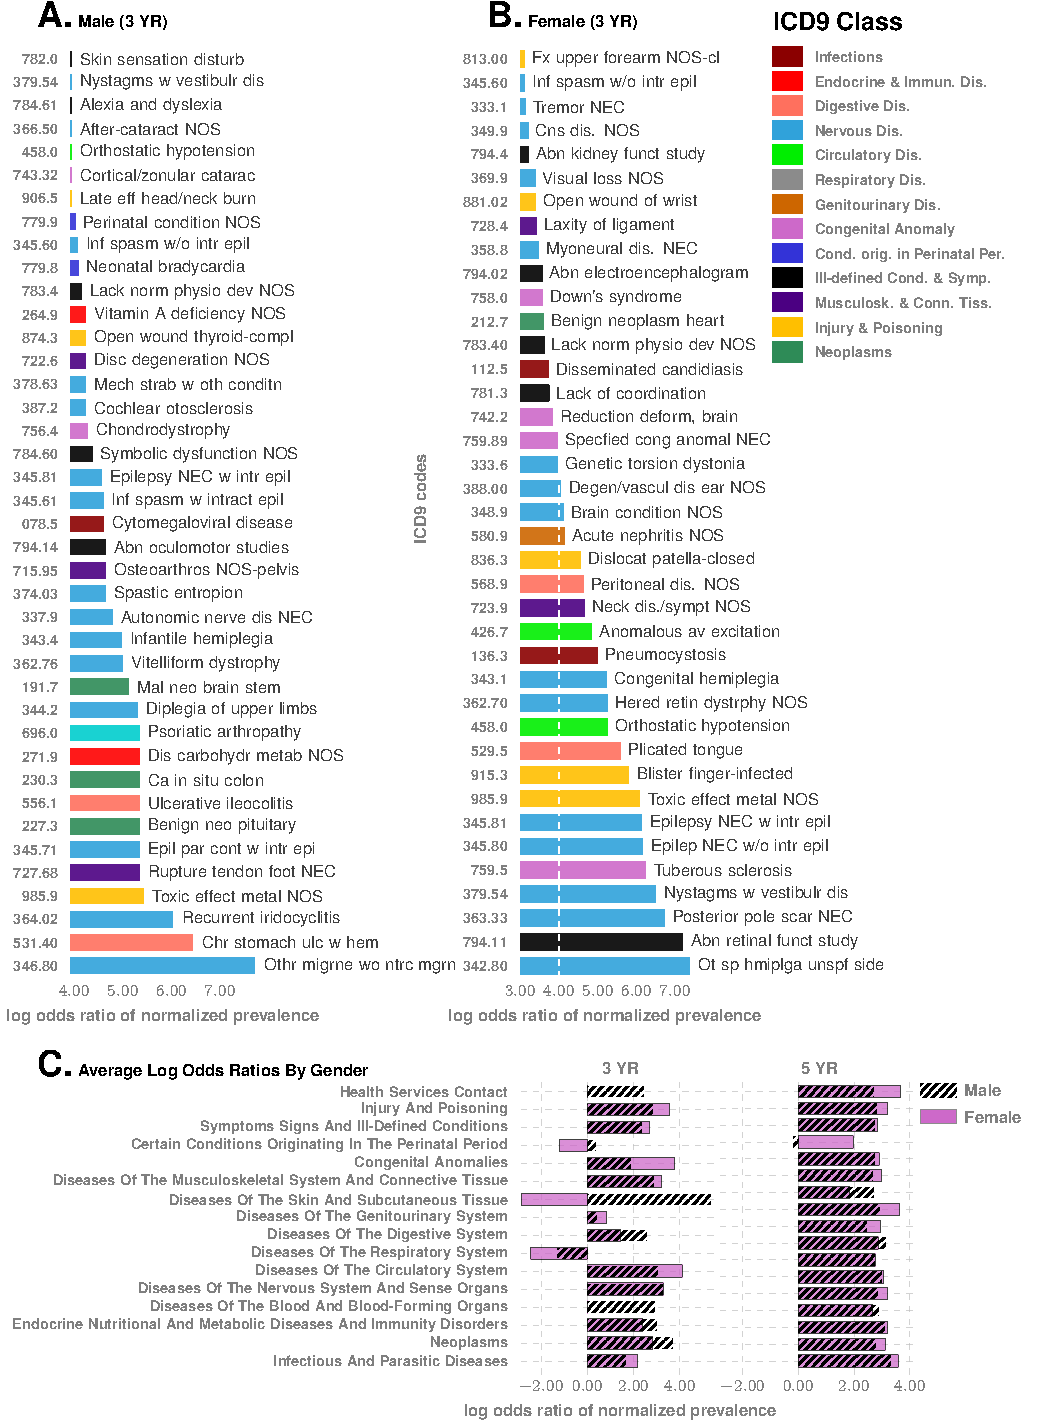
\includegraphics[width=0.99\textwidth]{Figures/External/comorbidA}
\fi
  \vspace{-5pt}
  
  \captionN{\textbf{Co-morbidity Patterns} Panel A and B. Difference in occurrence frequencies of diagnostic codes between true positive (TP) and true negative (TN) predictions. The dotted line on panel B shows the  abscissa lower cut-off in Panel A, illustrating the lower prevalence of codes in females. Panel C illustrates log-odds ratios for ICD9 disease categories at different ages. Importantly, the negative associations disappear when we consider older children, consistent with the lack of such reports in the literature which lack studies on very young cohorts. }\label{EXT-fig3}
  \vspace{-5pt}
  
\end{figure*}
\else
\refstepcounter{figure}\label{EXT-fig3}
\fi
% ###########################################################
% #############

%#################################### 
\begin{table}[!ht]
\centering

\mnp{.89\textwidth}{

\captionN{Boosted Sensitivity, Specificity and PPV Achieved at  \textbf{150 weeks}  Conditioned on M-CHAT/F Scores}\label{EXT-tabboost150}
  \vskip .5em

\begin{tabular} {L{.33in}|L{.33in}|L{.33in}|L{.33in}||L{.35in}|L{.35in}|L{.375in}||L{.375in}|L{.35in}|L{.35in}||L{.6in}}
\hline
\multicolumn{4}{c||}{\cellcolor{lightgray!60}M-CHAT/F Outcome}  & \multicolumn{3}{c||}{\mnp{.9in}{\vskip .2em global\\performance (Truven)\vskip .2em  } }&\multicolumn{3}{c||}{\mnp{1in}{\vskip .2em global\\performance\\(UCM)\vskip .2em }} &  \multirow{3}{*}{prevalence}\\\cline{0-9}
 0-2  NEG & 3-7  NEG & 3-7  POS & $\geq  8$  POS & \multirow{2}{*}{\mnp{.1in}{speci-ficity}} & \multirow{2}{*}{\mnp{.1in}{sensi-tivity}} &\multirow{2}{*}{PPV}& \multirow{2}{*}{\mnp{.1in}{speci-ficity}} & \multirow{2}{*}{\mnp{.1in}{sensi-tivity}} & \multirow{2}{*}{PPV} & \\\cline{0-3}
\multicolumn{4}{c}{\cellcolor{lightgray} specificity choices}  & & & &&&&\\\hline 
  0.28&0.66&0.93&0.97&0.95&0.64&0.224&0.95&0.577&0.206&0.022\\\hline 
0.31&0.67&0.9&0.97&0.95&0.641&0.223&0.95&0.577&0.205&0.022\\\hline 
0.54&0.86&0.97&0.99&0.98&0.494&0.361&0.98&0.393&0.31&0.022\\\hline 
0.41&0.89&0.96&0.99&0.98&0.493&0.362&0.98&0.391&0.311&0.022\\\hline 
0.31&0.61&0.86&0.98&0.95&0.808&0.219&0.95&0.713&0.198&0.017\\\hline 
0.33&0.6&0.86&0.98&0.95&0.809&0.218&0.95&0.715&0.197&0.017\\\hline 
0.66&0.95&0.98&0.99&0.98&0.574&0.337&0.98&0.417&0.269&0.017\\\hline 
0.53&0.97&0.98&0.99&0.98&0.573&0.337&0.98&0.412&0.267&0.017\\\hline 
0.54&0.91&0.97&0.99&0.978&0.615&0.322&0.978&0.499&0.278&0.017\\\hline 
0.52&0.92&0.97&0.99&0.978&0.612&0.324&0.978&0.492&0.278&0.017\\\hline 
 
\end{tabular}}

\vspace{10pt}

\mnp{.97\textwidth}{
  \captionN{Population Stratification Results on large M-CHAT/F Study(n=20,375)  reproduced from Guthrie $\etal$~\cite{pmid31562252} }\label{EXT-tabCHOP}
    \vskip .5em

  \begin{tabular}{C{.5in} | L{1.5in}|L{1in}|L{1in}|L{1in}||L{.5in}}\hline
 \bf \sffamily   Id &  \bf \sffamily Sub-population & \bf \sffamily Test Result & \bf \sffamily ASD positive & \bf \sffamily ASD Negative & \bf \sffamily Total \% \\\hline
   A &  M-CHAT/F $\geqq 8$ & Positive & 0.34\% & 0.64\% & 0.99\% \\\hline
  B &   M-CHAT/F $\in [3,7]$ & Positive (after follow-up)& 0.52\% & 4.39\% & 4.91\% \\\hline
 C &    M-CHAT/F $\in [3,7]$ & Negative (after follow-up)& 0.14\% & 3.1\% & 3.24\% \\\hline
  D &   M-CHAT/F $\in [0,2] $ & Negative & 1.22\% & 89.63\% & 90.86\% \\\hline\hline
    Total \%& &   &2.23\% & 97.77\% & 100\% \\\hline
    \end{tabular}
}

\vspace{10pt}

\mnp{.9\textwidth}{
  \captionN{$\gamma,\gamma'$ Computed from Population Stratification Recorded In  M-CHAT/F Study~\cite{pmid31562252} ($\rho=0.0223$) }\label{EXT-tabCHOP2}
    \vskip .5em

  \begin{tabular}{C{.5in} | L{1.35in} | L{1.5in}|L{.35in}|L{.35in}|L{.35in}|L{.35in}}\hline
 \bf \sffamily   Id  &  \bf \sffamily Sub-population& \bf \sffamily Test Result & $\beta_i$ & $\rho_i$ & \bf \sffamily $\gamma_i$ & \bf \sffamily $\gamma'_i$ \\\hline
   A & M-CHAT/F $\geqq 8$ &  Positive &.0099 & .3469 &.1540  & .0066 \\\hline
  B & M-CHAT/F $\in [3,7]$ & Positive (after follow-up)& .0491 & .1059 &.2331  & .0449 \\\hline
 C &   M-CHAT/F $\in [3,7]$ & Negative (after follow-up)& .0324 & .0432 &.0627  & .0317 \\\hline
  D &  M-CHAT/F $\in [0,2] $ & Negative & .9086 & .0134 &.5471  & .9168 \\\hline
    \end{tabular}}

\end{table}
%###############################################
%###############################################


\end{document}      
